\documentclass[12pt]{unbthesis}
\usepackage[left=4cm, right=2.5cm, top=2.5cm, bottom=2.5cm]{geometry}
\usepackage{graphicx}
% \usepackage[caption = false]{subfig}
% \usepackage[subfigure]{tocloft} % no number for Vita in ToC
\usepackage{fancyhdr}
\usepackage[english]{babel}
\usepackage[utf8]{inputenc}
\usepackage{csquotes}
\usepackage{footmisc}
\usepackage{algorithmic}
\usepackage{listings}
\usepackage{fancyvrb}
\usepackage[nottoc]{tocbibind}
\usepackage[hidelinks]{hyperref}
\usepackage{url}
\usepackage{dirtytalk}
\usepackage{listings}
\usepackage{xparse}
\usepackage{xcolor}
\usepackage{color}
\usepackage[linesnumbered, ruled, vlined]{algorithm2e}
\usepackage{tikz}
\usepackage{float}
\usepackage[toc,page]{appendix}
\usepackage{caption}
\usepackage{subcaption}
\usepackage[export]{adjustbox}
\usepackage{array}

\captionsetup[figure]{font=small,skip=0pt}
\captionsetup[lstlisting]{font=small,skip=0pt}

\usepackage{listingsutf8}

\lstdefinelanguage{docker}{
  keywords={FROM, RUN, COPY, ADD, ENTRYPOINT, CMD,  ENV, ARG, WORKDIR, EXPOSE, LABEL, USER, VOLUME, STOPSIGNAL, ONBUILD, MAINTAINER},
  keywordstyle=\color{blue}\bfseries,
  identifierstyle=\color{black},
  sensitive=false,
  comment=[l]{\#},
  commentstyle=\color{purple}\ttfamily,
  stringstyle=\color{red}\ttfamily,
  morestring=[b]',
  morestring=[b]"
}

\lstdefinelanguage{docker-compose}{
  keywords={image, environment, ports, container_name, ports, volumes, links},
  keywordstyle=\color{blue}\bfseries,
  identifierstyle=\color{black},
  sensitive=false,
  comment=[l]{\#},
  commentstyle=\color{purple}\ttfamily,
  stringstyle=\color{red}\ttfamily,
  morestring=[b]',
  morestring=[b]"
}
\lstdefinelanguage{docker-compose-2}{
  keywords={version, volumes, services},
  keywordstyle=\color{blue}\bfseries,
  keywords=[2]{image, environment, ports, container_name, ports, links, build},
  keywordstyle=[2]\color{olive}\bfseries,
  identifierstyle=\color{black},
  sensitive=false,
  comment=[l]{\#},
  commentstyle=\color{purple}\ttfamily,
  stringstyle=\color{red}\ttfamily,
  morestring=[b]',
  morestring=[b]"
}

\lstset{basicstyle=\ttfamily,
  showstringspaces=false,
  commentstyle=\color{red},
  keywordstyle=\color{blue},
  inputencoding=utf8,
  extendedchars=true
}

% \include{dockerlst.tex}

\definecolor{dkgreen}{rgb}{0,0.6,0}
\definecolor{gray}{rgb}{0.5,0.5,0.5}
\definecolor{mauve}{rgb}{0.58,0,0.82}
\definecolor{codegreen}{rgb}{0,0.6,0}
\definecolor{codegray}{rgb}{0.5,0.5,0.5}
\definecolor{codepurple}{rgb}{0.58,0,0.82}
\definecolor{backcolour}{rgb}{0.95,0.95,0.92}

\lstdefinestyle{CodeStyle}{
    backgroundcolor=\color{backcolour},   
    commentstyle=\color{codegreen},
    keywordstyle=\color{magenta},
    numberstyle=\tiny\color{codegray},
    stringstyle=\color{codepurple},
    basicstyle=\linespread{1}\ttfamily\footnotesize,
    breakatwhitespace=false,         
    breaklines=true,                 
    captionpos=b,                    
    keepspaces=true,                 
    numbers=left,                    
    numbersep=5pt,                  
    showspaces=false,                
    showstringspaces=false,
    showtabs=false,                  
    tabsize=2
}

\lstdefinestyle{CommandStyle}{
    backgroundcolor=\color{backcolour},   
    commentstyle=\color{codegreen},
    keywordstyle=\color{magenta},
    % numberstyle=\tiny\color{codegray},
    stringstyle=\color{codepurple},
    basicstyle=\ttfamily\scriptsize,
    breakatwhitespace=false,         
    breaklines=true,                 
    captionpos=b,                    
    keepspaces=true,                 
    % numbers=left,                    
    % numbersep=5pt,                  
    showspaces=false,                
    showstringspaces=false,
    showtabs=false,                  
    tabsize=2
}

% \lstset{style=CodeStyle}



\graphicspath{ {./Images/} }

\title{Behnam Fuzzer}
\author{Behnam Bojnordi Arbab}
\predegree{Previous Degrees (i.e. Degree, University, Year)\\
Bachelor of Computer Engineering, Ferdowsi University of Mashhad, 2015}
\degree{Master of Computer Science}
\gau{Computer Science}
\supervisor{Ali Ghorbani, Faculty of Computer Science}
\examboard{N/A}
\externalexam{N/A}
\date{Soon...!}
\copyrightyear{2020}
\setlength\parindent{0pt}
\newtheorem{theorem}{Theorem}[section]
\newtheorem{definition}{Definition}[section]
\newtheorem{lemma}{Lemma}[section]
\newtheorem{notation}{Notation}[section]

\NewDocumentCommand{\codeword}{v}{%
\texttt{\textcolor{blue}{#1}}%
}

\begin{document}
\unbtitlepage
\setcounter{secnumdepth}{3} \setcounter{tocdepth}{3}
\pagenumbering{roman} \setcounter{page}{1}

%%-------------Abstract-----------------
\doublespacing
\chapter*{Abstract}
\addcontentsline{toc}{chapter}{Abstract} 

Fuzz testing helps software security researchers investigate the existing vulnerabilities within programs in an automated fashion. AFL is a whitebox coverage-based fuzzer leveraging a genetic algorithm (GA) to search for vulnerabilities inside a program. The inputs to the program, which may affect the program's execution paths are the chromosomes of GA and the content of the files that make up the genes. AFL investigates code coverages for the program's executions on each input, and the findings with new coverage information are selected for more testing. This technique guides the fuzzer to discover more regions of code. Waffle, is an AFL-based fuzzer searching for executions with higher resource usages, such as execution time. Waffle searches for files that not only discover new regions of code but also require more resources to complete a run. Waffle modifies the instrumentation and fuzzing modules of AFL, with the intention of storing resource/time-consuming executions. To confirm the correctness of the modifications, the binaries are assessed, and the fuzzing procedure is monitored from a status screen. Finally, the performance of Waffle is compared to AFL-based fuzzers, and it is shown that Waffle discovers exhaustive executions effectively.
%% -----------Dedication----------------
\chapter*{Dedication}
\addcontentsline{toc}{chapter}{Dedication} Dedicated to knowledge.

%%-----------Acknowledgements---------------
\chapter*{Acknowledgements (if any)}
\addcontentsline{toc}{chapter}{Acknowledgments} Start writing here.
This is optional.


%%-----------Table of Contents------------------
\renewcommand{\contentsname}{Table of Contents}
\clearpage
\addcontentsline{toc}{chapter}{Table of Contents}
\tableofcontents{}
%%------------List of Tables----------------------
\clearpage
% \addcontentsline{toc}{chapter}{List of Tables}
\listoftables{}
%%------------List of Figures----------------------
\clearpage
% \addcontentsline{toc}{chapter}{List of Figures}
\listoffigures{}
%%-----------List of Symbols, Nomenclature or Abbreviation--------
\chapter*{List of Symbols, Nomenclature or
Abbreviations} \addcontentsline{toc}{chapter}{Abbreviations} Start
writing here. This is optional.
\begin{table}[!h]
\begin{tabular}{l l r}
$\sum$  &$\backslash$sum\\
$\bigcap$ &$\backslash$bigcap
\end{tabular}
\end{table}

%%-------------change single space to double space--------
\clearpage
\doublespacing
\pagenumbering{arabic}
\setcounter{page}{1}

\chapter{Introduction}
\label{chap:ch1}

\section{Introduction}
\label{sec:1.1}

\section{Summary of contributions}
\label{sec:1.2}

In this thesis, we introduce a fuzzer which searches for states of program with a high load on available resources. The main contributions of our work are as follows:

\begin{itemize}
    \item Injecting fuzzing-dependent instructions for monitoring the loads of a targeted program.
    \item An algorithm for increasing the resource usages, and as a result causing exhaustive executions.
    \item Testing our work with state-of-the-art fuzzers, and evaluate the benefit of using our fuzzer. 
\end{itemize}

\section{Thesis Organization}
\label{sec:1.3}


%%-----------Chapters start-------------------------------------
%%-----------Chapter 1------------------------------------------
\chapter{Background}
\label{chap:ch2}
%\setcounter{secnumdepth}{3} \pagenumbering{arabic}
%\setcounter{page}{1} \pagestyle{myheadings}
%\markboth{}{}\markright{} \rhead{\thepage} \setcounter{page}{1}
%\pagestyle{myheadings} \pagenumbering{arabic} \rhead{\thepage}
%\setcounter{page}{1}

\section{Introduction} \label{sec:2.1}

% ! In the first chapter, you should explain about the fuzzers, how they cover the implementation bugs and how their performances are.
% ! A vulnerability is a reproducable state of a program's execution, that the program fails to execute as expected. 

% TODO: Here, we explain the 

% TODO: How many papers in the fi

Fuzzing (short for fuzz testing) is a tool for \say{finding implementation bugs using malformed/semi-malformed data injection in an automated fashion}. Since late 80's, fuzz testing has proved to be a powerful tool for finding errors in a program. For instance, American Fuzzy Lopper (AFL), has found more than total of 330 vulnerabilities since 2013 to 2017 in more than 70 different programs \cite{afl_cve}. The research on fuzz testing has found its place in the software security testing. Liang et al. \cite{liang2018fuzzing} illustrates the growth of the primary studies from the following publishers: \textit{ACM digital library}, \textit{Elsevier ScienceDirect}, \textit{IEEEXplore digital library}, \textit{Springer online library}, \textit{Wiley InterScience}, \textit{USENIX}, and \textit{Semantic scholar}. The queries for the literature reviews are "fuzz testing", "fuzzing", "fuzzer", "random testing", or "swarm testing" as the keywords of the titles. Figure \ref{fig:fuzz_articles} presents the results of the mentioned study.

\begin{figure}[!t]
    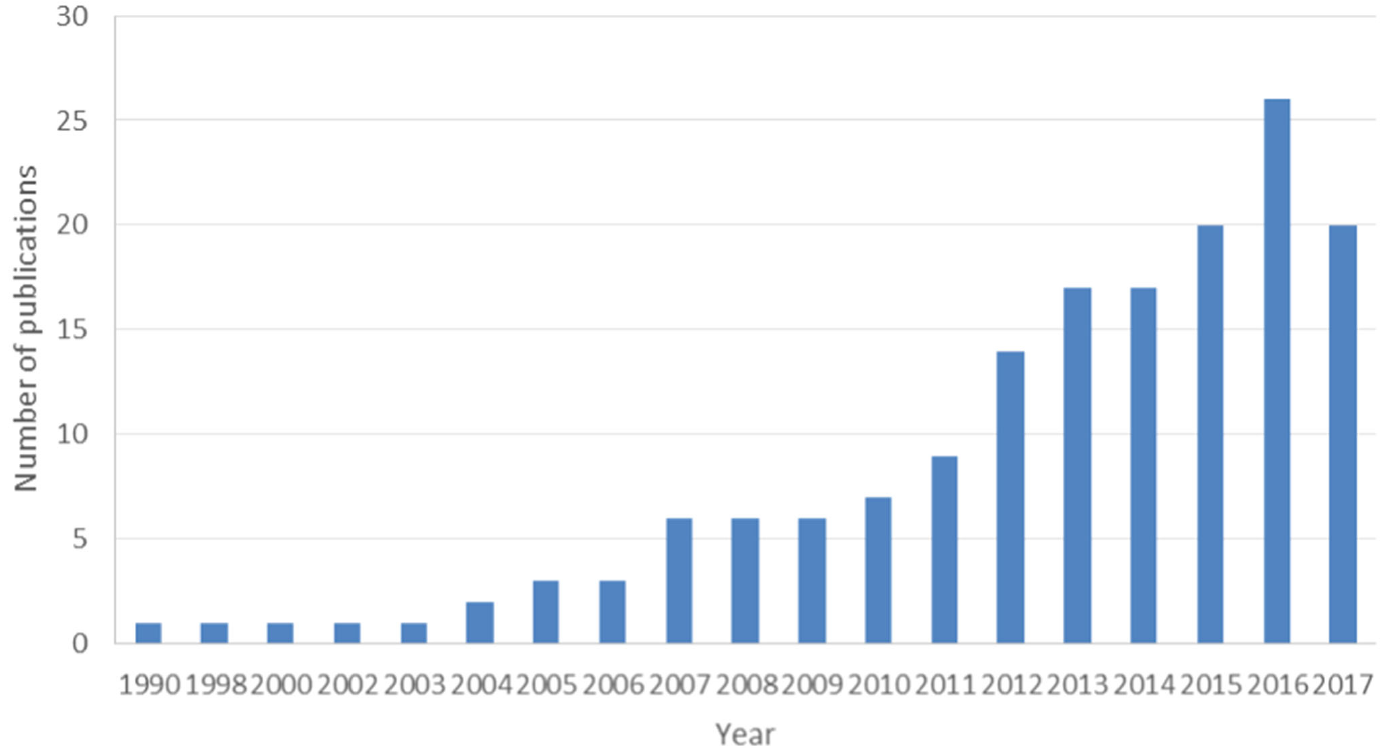
\includegraphics[width=\textwidth]{Chapter2/fuzz_articles.png}
    \centering
    \caption{Fuzzing papers published between January 1st, 1990 and June 30 2017. \cite{liang2018fuzzing}}
    \label{fig:fuzz_articles}
\end{figure}

The start and the termination of a \textit{run} are connected with a sequence of instructions. A successful execution behaves as the program is intended to run. An exception is a signal that is thrown, indicating an unexpected behavior. If the exception is not catched before the termination of the program, the operating system recieves an unfinished task with exception descriptions. From the OS's perspective, the program has crashed and could not finish it's execution properly. A software vulnerability is an unexpected state of the program that cannot be handled by the program. Different states of a program occur by different inputs that a program takes. The inputs such as \textit{environment variables}, \textit{file paths}, or other program's \textit{arguments} are mainly selected to search for the vulnerabilities. 

Fuzz testing a program is the repetitive executions of a target program with different inputs. Fuzz testing takes two main actions in the fuzzing procedure: the fuzzer \textit{generates test cases} for the target program, and each generated (fuzzed) test case is then passed to the program for \textit{execution}. A fuzzer gathers information out of each execution. A \textit{whitebox} fuzzer has access to the source code of the target program. \textit{Analyzing the source code}, \textit{monitoring the execution}, and \textit{validating the returned value of execution}, are of the capabilities of a whitebox fuzzer. Oppositely, a \textit{blackbox} fuzzer does not have any access to the source code, cannot analyze the execution, and does not check the result of the execution. Instead, a blackbox fuzzer focuses on executing more instances of the program, blindly. Fuzzers with at least one property from each one of the whitebox and blackbox fuzzers, are in the category of \textit{greybox} fuzzers.

The common strategies for generating new test cases include \textit{genetic algorithms}, \textit{coverage-based (coverage-guided) strategies}, \textit{symbolic execution}, \textit{taint analysis}, etc. Genetic algorithms (GA) are \textit{evolutionary algorithms} for generating solutions to \textit{search} and \textit{optimization problems} \cite{banzhaf1998genetic, whitley1994genetic}. GA has a population of solutions that their evaluations affect their surviveability for the next generation of the population. Inspired by the biological operations, GA processes the selected (survived) population and applies \textit{mutations} and other modifications on them, resulting in a new generation of the population. Coverage-guided strategy is a genetic algorithm that utilizes \textit{concrete analysis} of the \textit{execution-path} of a program. A concrete analysis investigates the runtime information of an executive program, and the graph of the executed instructions (execution-path) can be collected through this analysis. Symbolic executions can determine what constraints are affecting the execution-paths. A taint based analysis of a program tracks back the variables that cause a state of the executing program.

American Fuzzy Lopper (AFL) \cite{afl_git} is a coverage-based greybox fuzzer, that is originally considering the number of times each \textit{basicblock} of an execution is visited. Each basicblock is a sequence of instructions with no branches except the entry (jump in) and exit (jump out) of the sequence. AFL is published with two default tools for collecting the runtime information: \textit{LLVM} \cite{llvm} and \textit{QEMU} \cite{bellard2005qemu}. \say{The LLVM Project is a collection of modular and reusable compiler and toolchain technologies. Despite its name, LLVM has little to do with traditional virtual machines. The name "LLVM" itself is not an acronym; it is the full name of the project.} AFL acts as a \textbf{whitebox} fuzzer in \textit{llvm-mode}. In \textbf{llvm-mode}, AFL provides the recipe for compiling the target program with coverage information. The resulting compiler adds \textit{static instrumentations} to the program. Instrumentation is the process of injecting logging instructions into the program and the static instrumentation refers to the instrumentations applied on a binary before execution. The added instructions store the code-coverage and AFL can use them in Fuzzing. QEMU (Quick EMUlator) is an open-source emulator and virtualizer that helps AFL with \textit{dynamic instrumentation}. In dynamic instrumentation, the instructions are inserted in runtime and an emulator such as QEMU helps AFL with discovering the code-coverage \cite{afl_qemu}.

In this chapter, we begin with reviewing the previous works that lead to this thesis \ref{sec:2.2}. Next, we describe the implementation of AFL and its llvm-mode in \ref{sec:2.3}. We wrap up this chapter with conclusions.

\section{Literature Review} \label{sec:2.2}

% Talk about the meaning and history of fuzzing

\begin{figure}[!b]
    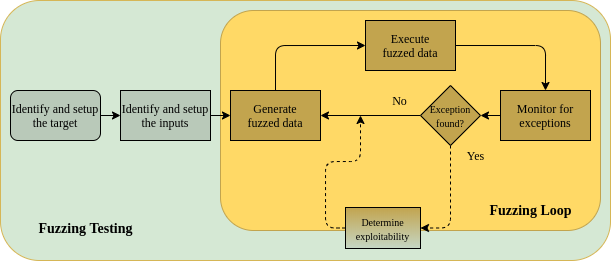
\includegraphics[width=\textwidth]{Chapter2/FuzzingPhases.png}
    \centering
    \caption{Fuzzing phases}
    \label{fig:fuzz_phases}
\end{figure} 

Sutton et al. \cite{sutton2007fuzzing} defined the procedure of fuzz testing, as shown in Figure \ref{fig:fuzz_phases}:
\begin{enumerate}
    \item Generally, the first stage is \textbf{to identify the target}. A target may be a software or a combination of software and hardware \cite{song2019periscope}. The targeted software is any program that is executed on a machine. For the rest of this article, a target is software.
    
    \item To execute the target program, we need to specify how the program parses the inputs. Inputs are a set of environmental variables, file formats, and any other parameters that affect the program's execution.
    
    A fuzzer needs a set of seeds for initialization. This set could be empty, and a fuzzer without any sample inputs may find valid fuzzed files out of thin air \cite{out_of_thin_air} that the target program considers them as valid.
    
    \item The fuzzing loop starts with generating fuzzed inputs. The fuzzer provides these files for the program to execute and process them.

    \item In this stage, the inputs are processed and executed. Depending on the resources needed for the target program's execution, this stage can be the bottleneck for the fuzzing process. The executions' interesting behavior and information are collected for the evolution of the inputs in future iterations.

    \item If an exceptional event happens during the program's execution and the program exits unsuccessfully, we say an exception is occurred. These exceptions are the vulnerabilities that may be exploitable and cause security problems. Handling an exception properly and pinpointing the inputs responsible for the exception is the primary purpose of this stage.
    
    \item The last stage of the fuzzing is evaluating the reported vulnerabilities. This evaluation explains whether the vulnerabilities are exploitable or not.

\end{enumerate}

A common feature in most of the fuzzers is the fuzzing loop which is looking for more valuable inputs. The stages may vary depending on the problem and goals of a fuzzer. We will walk over the stages of AFL as our fuzzer is based on AFL, and we will be back on the stages of fuzzing in the following sections.

\subsubsection*{Sample program}
To evaluate the performance of a fuzzer and assess the execution of it, the sample \textbf{C} code is implemented. (Listing \ref{lst:sample_vul}) \cite{sample_code_ref}

\lstinputlisting[language=C++,style=CodeStyle,caption={Sample vulnerable program},label={lst:sample_vul}]{Codes/Chapter2/sample_vul.c}

The sample program has a \textbf{Heap buffer overflow vulnerability}. If we compile this code with GCC and debugging flags, the vulnerability stays hidden and the program executes without any errors:

\lstinputlisting[language=bash,style=CommandStyle,label={lst:exec1}]{Codes/Chapter2/exec_1.txt}

One way to detect the prior vulnerability, is to add AddressSanitizer flag for the compilation \cite{address_san}. ASan is a fast memory error detector. This tool uses memory poisoning for the detection of a heap buffer overflow. (You can find more features of this tool in the reference) \cite{serebryany2012addresssanitizer}

After we provide the ASan flag for the compilation, we face an error with the same input as the previous example (Listing \ref{lst:exec2}):

\lstinputlisting[language=bash,style=CommandStyle,label={lst:exec2}]{Codes/Chapter2/exec_2.txt}

The detection of the vulnerabilities or any other exceptions, signals the operating system for a misbehaviour from the program. A fuzzer would need this signal to evaluate the execution of the target program.

\subsubsection*{Black/Grey/White-box fuzzing}

The \textit{colorful} representation of fuzzers depends on how much information we can collect from any execution of the target. In a blackbox fuzzing, we do not gather any information from the execution, and the fuzzing tries new inputs expecting an error to occur.

\lstinputlisting[language=bash,style=CommandStyle,label={lst:bbox}]{Codes/Chapter2/bbox_fuzz.txt}

% \vspace{1.5\baselineskip}

% Blackbox fuzzer
The introduced fuzzer by Miller \cite{miller1990empirical} was of the very first naive blackbox fuzzers targeting a collection of Unix utilities on different Unix versions. It runs the fuzzing for different lengths of inputs for each utility (of the total 88 utilities) and expects a \textbf{crash}, \textbf{hang}, or a \textbf{succeed} after the execution of the program. The generation of inputs is by the mutation of the inputs' content, and the target program is a blackbox for the fuzzer. As a result, this fuzzer is a mutation-based blackbox fuzzer.


One of the \textbf{downsides} of the blackbox fuzzing is that the program may face some branches with \textbf{magic values}, constraining the variable to a specific set of values; the fuzzer has to apply the exact magic value, which may have a very low probability - it is almost impossible to generate a specific 1 KB string of bytes randomly.. In \cite{banks2006snooze} and \cite{gascon2015pulsar} a set of network protocols are fuzzed in a blackbox manner, but as the target is specified, the performance is enhanced drastically. Any application on the web may be considered a blackboxed program as well, so as \cite{doupe2012enemy} and \cite{duchene2012xss} have targeted web applications and found ways to attack some the websites, looking for different vulnerabilities, such as XSS.

% Whitebox fuzzers
\vspace{1.5\baselineskip}

Whitebox fuzzing works with the source code of the target. In this technique, an \textbf{instrumentation} is applied before the compilation of the program. Instrumeting a program with debugging instructions, is the procedure of injecting new instructions into the resulting binary, without affecting the logic of the program. We will analyze the instrumentations more in the \nameref{sec:2-llvm} section.

The following snippet of code shows an example of such execution \ref{lst:wbox}. \textit{whitebox-instr-c} compiles the program with the required instrumentations and \textit{whitebox-fuzzer} fuzzes the program appropriately.

\lstinputlisting[language=bash,style=CommandStyle,label={lst:wbox}]{Codes/Chapter2/wbox_fuzz.txt}

SAGE, a whitebox fuzzer, was developed as an alternative to blackbox fuzzing to cover the lacks of blackbox fuzzers \cite{godefroid2012sage}. With the benefit of having the source code and internal knowledge for fuzzing, a whitebox fuzzer can leverage symbolic constraints for symbolic analysis to solve the constraints (such as magic values) in the program \cite{cadar2011symbolic}. It can also use dynamic and concolic execution \cite{stephens2016driller} and use taint analysis to locate the regions of seed files influencing values used by program \cite{ganesh2009taint}. In addition, a whitebox fuzzer can find the grammar for parsing the input files without any prior knowledge \cite{godefroid2008grammar}. It is a noticeable performance enhancement as we have the source code.

\vspace{1.5\baselineskip}

Greybox fuzzing resides between whitebox and blackbox fuzzing, as we only have partial knowledge about the internals of the target program. We do not have the source code, but we have some knowledge about the program (for instance, we have the binary file), and as a result, we have the instructions of the program (\ref{lst:gbox}):

\lstinputlisting[language=bash,style=CommandStyle,label={lst:gbox}]{Codes/Chapter2/gbox_fuzz.txt}

AFL \say{allows you to build a standalone feature that leverages the QEMU "user emulation" mode and allows callers to obtain instrumentation output for black-box, closed-source binaries}, working as a greybox fuzzer \cite{afl_qemu}. The instrumentation using \textbf{QEMU} on a binary has an average performance cost of 2-5x, which is better than other tools such as \textbf{DynamoRIO} and \textbf{PIN}.

\subsubsection*{Coverage-based fuzzing}

Coverage-based fuzzing is technique for fuzz testing that instruments the target without analyzing the logic of the program. In a greybox and whitebox coverage-based fuzzing, the instrumentation detects the different paths of the executions \cite{liang2018fuzzing}. AFL instruments the program with only the coverage information (section \nameref{sec:2-afl}).

The instrumentation can collect execution's data such as data coverage, statement coverage, block coverage, decision coverage, and path coverage \cite{yang2009survey}. Bohme et al. \cite{bohme2017coverage} introduced a coverage-based greybox fuzzer that extends AFL and benefits from the Markov Chain model. The fuzzer calculates the \textbf{energy} of the inputs based on the potency of a path for the discovery of new paths.

In another article by Bohme et al. \cite{bohme2017directed}, they introduce their directed fuzzing by the idea of checking the code-coverage for providing inputs that guide the program execution toward some targeted locations. Some of the applications of such a fuzzing approach are patch testing and crash reproduction, which has different use cases compared to a non-directed coverage-based fuzzers.

\subsubsection*{Performance fuzzing}

The \textbf{types} of vulnerabilities that a fuzzer is involved with may be different from other fuzzers. For example, AFL looks for crashes or hangs by selecting and mutating the inputs, and at the same time, it considers the code coverage, size of the inputs, and each execution time of the target program. PerfFuzz \cite{lemieux2018perffuzz} is a greybox fuzzer based on AFL, which aims to generate inputs for executions with higher \textbf{execution time} while using most of the features of AFL in code exploration. PerfFuzz counts how many times each of the edges of the control flow graph (CFG) is executed. Using SlowFuzz \cite{petsios2017slowfuzz}, we can consider any type of resource as a feature to detect the worst-case scenarios (inputs) for a given program. In another project based on AFL, Memlock \cite{wen2020memlock} investigates memory exhaustion by calculating the maximum runtime memory required during executions. A disadvantage in previous works in performance is that the development of the fuzzer for considering different instructions is cumbersome.

\vspace{1.5\baselineskip}

\textbf{Waffle (What An Amazing AFL - WAAAFL)} is a coverage-based whitebox fuzzer that is based on AFL's base code. Waffle leverages \textbf{visitors} to collect the stats of different instructions during the execution. To learn more about Waffle, we study the features we benefit from the LLVM, as well as the current features of AFL that help us in reaching the goals of this thesis.

\section{LLVM} \label{sec:2-llvm}

% TODO: update llvm information in references
\say{The LLVM Project is a collection of modular and reusable compiler and toolchain technologies. The LLVM project has multiple components. The core of the project is itself called “LLVM.” This project contains all of the tools, libraries, and header files needed to process intermediate representations and converts them into object files. Tools include an assembler, disassembler, bitcode analyzer, and bitcode optimizer.} \cite{llvm,lattner2004llvm}

\vspace{\baselineskip}

LLVM can be used as a compiler framework, separated into "front-end" and "back-end." The front-end contains the lexers and parsers, and it accepts the source code to a program and returns the \textbf{intermediate representation (IR)} of the program. The back-end converts the IR into machine language.

\vspace{\baselineskip}

For instrumentation, we insert the logging instructions into each basic block of the program in the front-end. \textbf{Clang} is part of the LLVM toolchain for compiling C/C++ source code. By definition, \say{\textbf{clang} is a C, C++, and Objective-C compiler that encompasses preprocessing, parsing, optimization, code generation, assembly, and linking.}\cite{clang} We extend the phases of compilation so that we are injecting the instructions in compilation. 

\vspace{\baselineskip}

LLVM converts an \textbf{IR} of a program into machine language instructions. The structure of the LLVM project is shown in Figure \ref{fig:llvm}:

\begin{figure}[htpb]
    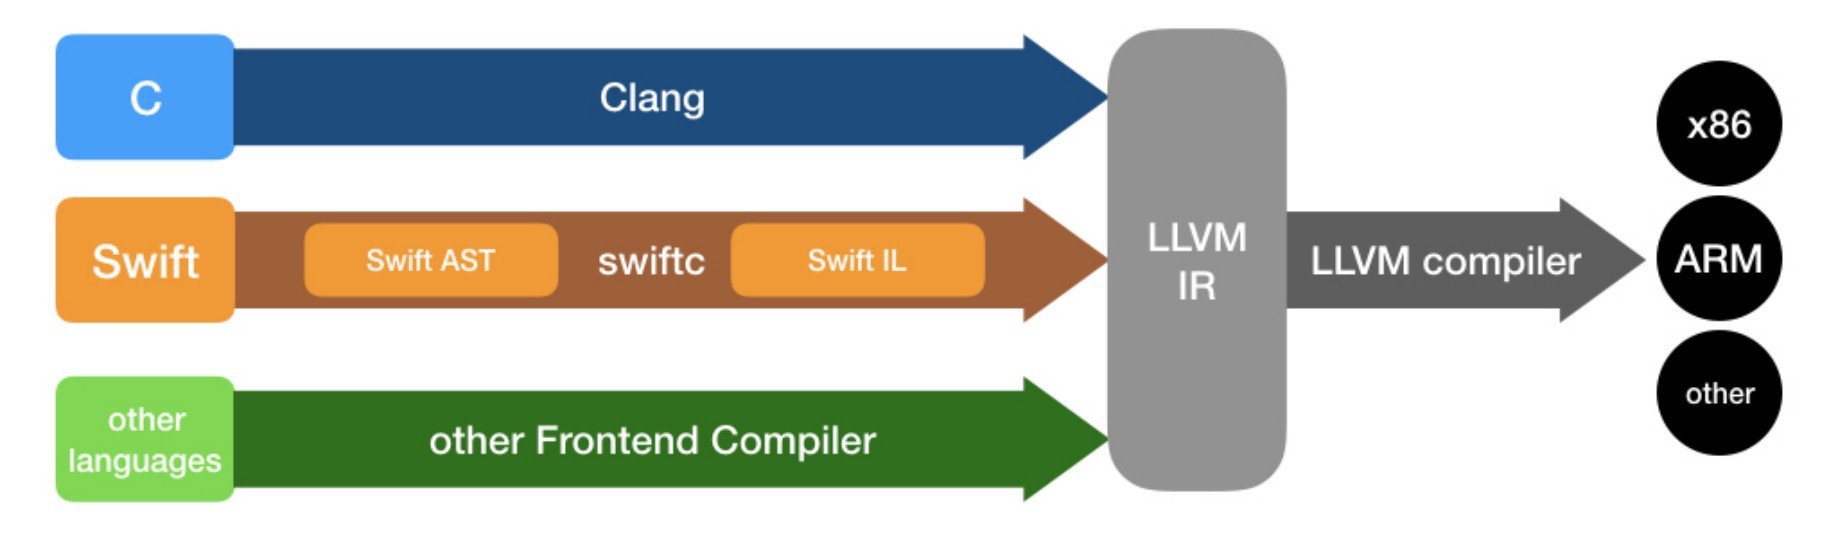
\includegraphics[width=\textwidth]{Chapter2/llvm.png}
    \centering
    \captionsetup{justification=centering}
    \caption{LLVM architecture: A front-end compiler generates the LLVM IR, and then it is converted into machine code \cite{omni_sci}}
    \label{fig:llvm}
\end{figure}

The instrumentation is applied before the IR generation, and the LLVM IR is fed into the LLVM compiler to generate the machine-specific instructions. As our instrumentation does not affect the LLVM IR compilation, we will not investigate the generated IR.


% Instrumentation
\subsection{Instrumentation and coverage measurements}
\label{instrumentation}

Waffle is based on AFL and we are extending the AFL's instrumentation in our work. The goal of using instrumentation for AFL is to differentiate code coverages. There are two techniques for instrumentation in AFL:

\begin{enumerate}
  \item \textit{$llvm\_mode$}: AFL takes the source code and an instrumentation recipe and generates the instrumented binary of the target program.
  \item \textit{$qemu\_mode$}: AFL leverages the QEMU mode to obtain instrumentation output for closed-source binaries. We don't use this mode in this thesis.
\end{enumerate}

In the LLVM recipe, we instantiate the bitmap and assign it to the shared memory for modifications. The remaining instructions for the recipe will be applied on the basic blocks in \textbf{AFLCoverage} module. This module takes effect in compilation of the program before the generation of IR. We can see some of the implementation of this \textbf{pass} in Listing \ref{lst:afl-llvm}:

\lstinputlisting[language=C++,style=CodeStyle,label={lst:afl-llvm},caption={AFLCoverage module}]{Codes/Chapter2/afl_llvm_pass.cpp}

The recipe for instrumentation fills out the coverage bitmap with the hash values of the paths executed. The instructions are as followed:

\begin{lstlisting}[language=C++,style=CodeStyle,label={lst:hash},caption={Select element and update in shared\_mem}]
  cur_location = <COMPILE_TIME_RANDOM>;
  shared_mem[cur_location ^ prev_location]++; 
  prev_location = cur_location >> 1;
\end{lstlisting}

AFL instruments by adding these instructions into basic blocks. First, a random value is assigned to \textit{curr\_location}. Next, it is XORed with the previous location's value, \textit{prev\_location}, and the resulting value is the location on \textit{shared\_mem}, the \textit{coverage bitmap}, which is incremented by one. The third and final instruction is reseting the \textit{prev\_location} to a new value.

\vspace{\baselineskip}

When AFL runs the instrumented program, every time an instrumented basic block is executed, a dedicated location of $shared\_mem$ in the bitmap is incremented. This algorithm recognizes the different paths that AFL runs through. For instance, in figure \ref{fig:instrumentation}, suppose that we have an instrumented program with the random values which is set in compile time. An execution that walks over basic blocks $1\rightarrow2\rightarrow5$ will increase the value of the corresponding locations by 1; for instance, an increment on $shared\_mem[14287 \oplus 23765]$ is applied for the transition of $1\rightarrow2$ and $shared\_mem[7143 \oplus 21689]$ for $2\rightarrow5$. We can see that the paths $1\rightarrow3\rightarrow4\rightarrow5$ and $1\rightarrow3\rightarrow4\rightarrow3\rightarrow4\rightarrow5$ (which contains a loop), set different locations on bitmap.


\begin{figure}[htpb]
    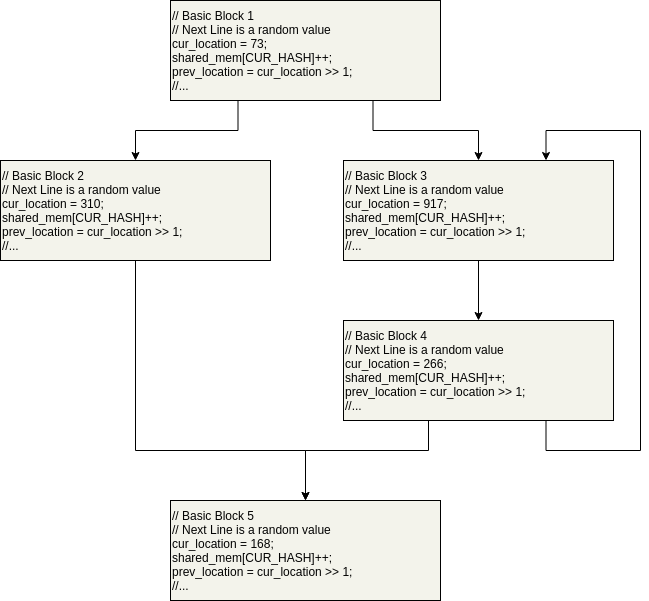
\includegraphics[width=\textwidth]{Chapter2/instrumentation.png}
    \centering
    \captionsetup{justification=centering}
    \caption{Example for instrumented basic blocks}
    \label{fig:instrumentation}
\end{figure}

AFL uses this coverage feature for discovering new inputs with new code coverages.

\subsubsection*{Visitor functions}

\say{Instruction visitors are used when you want to perform different actions for different kinds of instructions without having to use lots of casts and a big switch statement (in your code, that is). \cite{inst_visitor}} 

\lstinputlisting[language=C++,style=CodeStyle,label={lst:visitors},caption={Visitors example}]{Codes/Chapter2/visitor.cpp}

The specified range can be any two iterators, which can be a Module, Function, BasicBlock, Instruction or any other range between two instruction addresses.


\section{AFL} \label{sec:2-afl}

Michal Zalewski initially developed American Fuzzy Lopper. He introduces this open-source project as \say{a security-oriented fuzzer that employs a novel type of compile-time instrumentation and genetic algorithms to automatically discover clean, interesting test inputs that trigger new internal states of the targeted binary. This substantially improves the functional coverage for the fuzzed code. The compact synthesized corpora produced by the tool help seed other, more labor- or resource-intensive testing regimes down the road.} \cite{zalewski2014american}

AFL is designed to perform \textbf{fast} and \textbf{reliable}, and at the same time, benefit from the \textbf{simplicity} and \textbf{chainability} of the fuzzer \cite{about_afl}:

\begin{itemize}
    \item \textbf{Speed:} Avoiding the time-consuming operations and increasing the number of executions over time.
    \item \textbf{Reliability:} AFL takes strategies that are program-agnostic, leveraging only the coverage metrics for more discoveries. This feature helps the fuzzer to perform consistent in finding the vulnerabilities in different programs.
    \item \textbf{Simplicity:} AFL provides different options, helping the users enhance the fuzz testing in a straightforward and meaningful way. 
    \item \textbf{Chainability:} AFL can test any binary which is executable, and is not constrained by the target software. A driver for the target program can connect the binary to the fuzzer.
\end{itemize}

\textit{afl-fuzz.c} has the instructions for fuzzing the target instrumented-program. The Algorithm \ref{algo:afl} illustrates a brief pseudocode of the execution of \textit{afl-fuzz}:

% main
%     initialize the fuzzer
%     while fuzzing is not terminated:
%         cull the queue of tests and update the bitmap
%         select the first entity of the queue, as E
%         fuzz(E)

% calibrate:
%     /* Calibrate a new test case. This is done when processing the input directory
%    to warn about flaky or otherwise problematic test cases early on; and when
%    new paths are discovered to detect variable behavior and so on. */

% trimming:
%     /* Trim all new test cases to save cycles when doing deterministic checks. The
%    trimmer uses power-of-two increments somewhere between 1/16 and 1/1024 of
%    file size, to keep the stage short and sweet. */

\begin{algorithm}
    % \DontPrintSemicolon % Some LaTeX compilers require you to use \dontprintsemicolon instead
    \KwIn{\textbf{$in\_dir$}, \textbf{$out\_dir$}, $instrumented$ \textbf{$Target$}}
    initialize fuzzer\;
    \While{fuzzing is not terminated} {
      $cull\_queue()$\;
      $Entry \leftarrow q.first\_entry()$\;
      $fuzz\_one(Entry)$\;
    }
    \caption{afl-fuzz}
    \label{algo:afl}
\end{algorithm}

After the environmental initializations, the fuzzing loop continues until receiving a termination signal. In every iteration of the loop, AFL first culls the corpus of the generated entries. This method assigns a \textbf{favor-factor} (Eq \ref{eq:afl_fav_fac}) to each queue\_entry and marks the \textbf{favorite entries}, as they execute faster and the size of the files are smaller than the rest of the corpus. AFL finds a favorable path for \say{having a minimal set of paths that trigger all the bits seen in the bitmap so far, and focus on fuzzing them at the expense of the rest.} \cite{afl_git} 
\begin{equation}
    fav\_factor = e.exec\_time \times e.length
    \label{eq:afl_fav_fac}
\end{equation}

An entry is selected after culling the queue. AFL evolves the input corpus by generating new entries out of the selected input entry - \texttt{fuzz\_one()}. 

\subsubsection*{fuzz\_one()}

% fuzz
%     calibrate the test case
%     trim the test cases (if needed)
%     calculate the performance score
%     bitflip
%     interesting values and dictionary usage
%     random havoc

\begin{algorithm}
    \KwIn{\textbf{$queue Entry$}}
    $test\_case \leftarrow Entry.test\_case$
    $calibrate(test\_case)$\;
    $bitflip(test\_case)$\;
    $save\_if\_interesting(test\_case)$\;
    $random\_havoc(test\_case)$\;

    \caption{$fuzz\_one$: Fuzz one Entry}
    \label{algo:fuzzone}
\end{algorithm}

Fuzzing a single entry requires the calibration of the test-cases; calibration helps AFL in evaluating the stats of the current entry. This evaluation is stored in \texttt{perf\_score}, and the number of trials for generating new inputs from the \textbf{random\_havoc} stage is calculated using the \texttt{perf\_score}. AFL, as a coverage-based fuzzer, assigns higher performance score for the entries that are executed faster and have bigger bitmaps.

The evolutionary algorithms for generating new entries are applied in two stages: \textbf{deterministic} and \textbf{random\_havoc} stages. As shown in Algorithm \ref{algo:fuzzone}, AFL initially tries the basic, deterministic algorithms. These algorithms are executed for a specific number of times, in the same order, and once for each fuzzing trial. . Bit-flipping, byte-flipping, simple arithmetic operations, using known integers and values from dictionaries, are a sequence of mutations that AFL applies on an entry in \textbf{deterministic} stage. Each one of the above operations tweak a small portion of the fuzzed input, and does not modify the file in large portions - up to 32 bits changes in each tweak.

The \textbf{havoc} stage is a cycle of stacked random tweaks. AFL assesses the current entry to insert into the queue. Each mutation is selected randomly and with a higher \texttt{perf\_score}, this stage continues more fuzzing over the current entry. The \texttt{random\_havoc} stage consists techniques such as bit flips, overwriting with random and interesting integers, block deletion, block duplication, and (if supplied) assorted dictionary-related operations \cite{afl_userguide}. An abstract implementation of the \texttt{havoc\_stage} can be found in Appendix \ref{app:havoc}.

\subsubsection*{calculate\_score()}
\label{sub:calc_score}

This function calculates how much AFL desires to iterate in havoc stage, for the current entry. By default, AFL is interested in fuzzing an input with less execution-time, and simultaneously, showing more coverage, and it's generation depth is higher. The depth of a child entry is one more than the depth of it's parent. For more information, check the following abstraction of the function [Listing \ref{lst:calc_score}]: 

\lstinputlisting[language=C,style=CodeStyle,label={lst:calc_score},caption={An abstract implementation of calculate\_score()}]{Codes/Chapter2/calculate_score.c}

\subsubsection*{common\_fuzz\_stuff()}
The newly fuzzed (generated) inputs must pass \texttt{common\_fuzz\_stuff()} for validating and instantiating a \texttt{queue\_entry}. The validation checks the length of the fuzzed file, executes the program and keeps the exit-value of the execution. In the end, AFL calls \texttt{save\_if\_interesting()} to insert the entry into the queue, if it is interesting. The function \texttt{has\_new\_bits()} considers how interesting an entry is.

\lstinputlisting[language=C,style=CodeStyle,label={lst:common_stuff},caption={An abstract implementation of common\_fuzz\_stuff()}]{Codes/Chapter2/common_fuzz_stuff.c}

\subsubsection*{has\_new\_bits()}
AFL calls this function after each execution of the program, and the optimization of this code participates an important role.

\lstinputlisting[language=C,style=CodeStyle,label={lst:has_new_bits},caption={The implementation of has\_new\_bits()}]{Codes/Chapter2/has_new_bits.c}

\subsubsection*{Status screen}

The \textbf{status screen} is a UI for the status of the fuzzing procedure. As it is shown in Figure \ref{fig:status_screen}, there are multiple stats provided in real-time updates:
    
\begin{figure}[!b]
    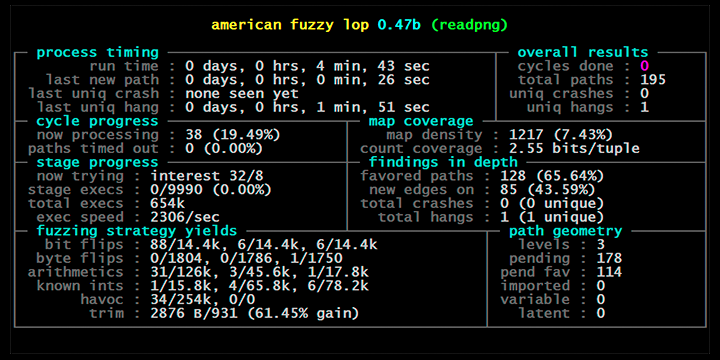
\includegraphics[width=\textwidth]{Chapter2/afl_screen.png}
    \centering
    \caption{AFL status screen}
    \label{fig:status_screen}
\end{figure} 

\begin{enumerate}
    \item \textbf{Process timing}: This section tells about how long the fuzzing process is running.
    \item \textbf{Overall results}: A simplified information about the progress of AFL in finding paths, hangs, and crashes. 
    \item \textbf{Cycle progress}: As mentioned before, AFL takes one input and repeats mutating it for a while. This section shows the information about the current cycle that the fuzzer is working on.
    \item \textbf{Map coverage}: \say{The section provides some trivia about the coverage observed by the instrumentation embedded in the target binary. The first line in the box tells you how many branches we have already hit, in proportion to how much the bitmap can hold. The number on the left describes the current input; the one on the right is the entire input corpus's value. The other line deals with the variability in tuple hit counts seen in the binary. In essence, if every taken branch is always taken a fixed number of times for all the inputs we have tried, this will read "1.00". As we manage to trigger other hit counts for every branch, the needle will start to move toward "8.00" (every bit in the 8-bit map hit) but will probably never reach that extreme. 
    
    Together, the values can help compare the coverage of several different fuzzing jobs that rely on the same instrumented binary.
    }
    \item \textbf{Stage progress}: The information about the current mutation stage is briefly provided here.
    \item \textbf{Findings in depth}: The crashes and hangs and any other findings (here we have the other information about the coverage) are presented in this section.
    \item \textbf{Fuzzing strategy yields}: To illustrate more stats about the strategies used since the beginning of fuzzing, and for comparison of those strategies, AFL keeps track of how many paths were explored, in proportion to the number of executions attempted, for each of the fuzzing strategies.
    \item \textbf{Path geometry}: The information about the inputs and their depths, which says how many generations of different paths were produced in the process. For instance, we call the seeds we provided for fuzzing the "level 1" inputs. Next, a new set of inputs is generated as "level 2", the inputs derived from "level 2" are "level 3," and so on.
\end{enumerate}

\subsubsection*{Start Fuzzing}

AFL requires the instrumented binary for execution. To start the instrumentation, AFL uses \textit{afl-clang}, which is built with the coverage recipe included. The following command instruments the sample program \ref{lst:sample_vul}:

\begin{lstlisting}[language=bash,style=CommandStyle,caption=Instrument $sample\_vul$.c]
    afl-clang sample_vul.c -o sample_vul_i
\end{lstlisting}

Now AFL can run this program in \textit{afl-fuzz} with the coverage instrumentations.

\begin{lstlisting}[language=bash,style=CommandStyle,caption=Execute AFL]
  # afl-fuzz -i <in_dir> -o <out_dir> [options] -- /path/to/fuzzed/app [params]
  afl-fuzz -i in_dir -o out_dir -- ./sample_vul_i
\end{lstlisting}

The fuzzing continues until the fuzz testing is stopped using a termination signal. Pressing \textit{Ctrl+C} is a common command for this purpose. All of the recorded information are accessed through the output directory \textit{out\_dir}.

% \newpage
\section{Concluding remarks}

In this chapter, we reviewed the previous works that inspired us for the development of Waffle. We covered these topics:

\begin{itemize}
    \item A brief description of the previous fuzzers.
    \item The recognition of whitebox, blackbox, and greybox fuzzers.
    \item Code coverage technique and its applications in fuzz testing were explained.
    \item We briefly explained the instrumentation with LLVM and visitor functions.
    \item We dug into the state-of-the-art fuzzer, AFL, and researched its fuzzing procedure.
\end{itemize}

In the next chapter we will explore more into the modifications we applied on AFL to achieve Waffle.

%%-----------Chapters start-------------------------------------
%%-----------Chapter 1------------------------------------------
\chapter{Proposed Fuzzer}
\label{chap:3}
%\setcounter{secnumdepth}{3} \pagenumbering{arabic}
%\setcounter{page}{1} \pagestyle{myheadings}
%\markboth{}{}\markright{} \rhead{\thepage} \setcounter{page}{1}
%\pagestyle{myheadings} \pagenumbering{arabic} \rhead{\thepage}
%\setcounter{page}{1}

% TODO: describe the 
% \section{Theoritical aspects}
% TODO: for instance, talking about how the Memfuzz is working
% TODO: talk about how our approach is going to be injected to the procedure of memfuzz

\section{Introduction}
In this chapter a new fuzzer is introduced, that is capable of finding the vulnerabilities related to (theoretically) any resource's exhaustion. The first section explains a motivating example leading to our proposed fuzzer. The fuzzer is based on AFL and uses the implementation of Memlock for memory usage assessments. For monitoring the resources, we use compile-time instrumentation of the target program using LLVM's APIs; we take advantage of \textbf{visiting} APIs that let us keep track of any type of instructions defined for LLVM. As a result, the instructions related to any resource are counted and this information is later used in the fuzzing stage. The vulnerabilities found by our fuzzer are then tested for exploitability. The short-comings and performance expectations of our fuzzer are investigated before we conclude this chapter.

We will call our proposed fuzzer \textbf{Waffle}, which is derived from \textbf{What An Amazing AFL} - WAAAFL! The summary of our contributions are as follows:

\begin{itemize}
    \item A new instrumentation for collecting runtime information about resource usages, i.e. memory and time.
    \item A new fuzz testing algorithm for collectively considering the former features of AFL and Memlock, as well as the features we introduce in Waffle.
\end{itemize}


% To have a more systematic proposal, make it look like you are selling your product to someone, or starting a startup ;)
\section{Motivating example}
\label{sec:3-motive}

The number of effective instructions can affect on the time complexity of a program. To exemplify our problem, we pick a program that has a variety of different execution-times, based on the inputs we provide for the program. 

Quicksort \cite{hoare1962quicksort} is a well-known fast algorithm for sorting a list of numbers. This divide-and-conquer algorithm selects a pivot and finds the position of the pivot on the list. After the selection, the other numbers of the list are swapped, until all the numbers that are less than the pivot are on one side, and the rest are on the other side of the pivot. Then A quicksort is called on each side, and we continue until there is no more unknown position for the numbers in the final sorted list.

This algorithm has a best-case scenario with $\mathcal{O}(n\log{}n)$ for the time complexity, and the worst-case occurs happens in $\mathcal{O}(n^2)$. The worst scenario is when we select the pivot and all other numbers are not swapped; as a result, we have to try the remaining elements of the list before the selection of the next pivot. The best-case scenario occurs when the pivot splits the list into two partitions that the difference between the length of the partitions is less than or equal to one. The average time complexity is $\mathcal{O}(n\log{}n)$.

The following code is an implementation of \textbf{quicksort} in C language:

\lstinputlisting[language=C,style=CodeStyle,label={lst:qsort},caption={Quicksort}]{Codes/Chapter3/quicksort.c}

We will consider testing the above code with Waffle in the next chapter.

\section{Instrumentation}
\label{sec:3-instr}

\subsubsection*{waffle-llvm-rt.o.c}

We initialize the instrumentation with setting up the shared memory for Waffle (Listing \ref{lst:llvm-rt}):

\lstinputlisting[language=C,style=CodeStyle,label={lst:llvm-rt},caption={LLVM instrumentation bootstrap}]{Codes/Chapter3/waffle-llvm-rt.o.c}

\texttt{\_\_wafl\_area\_ptr} is the region that is allocated for counting the instructions, and is later shared when the instrumented program is running in fuzz testing.

The size of the bitmap \texttt{\_\_wafl\_icnt\_ptr} is equal to $ICNT\_SIZE=2^{16}$; the size of the bitmaps are equal in both AFL and Waffle.

\subsubsection*{wafl-llvm-pass.so.cc}

Next, we inject our instrumentation into the program. As mentioned in the previous chapter, this stage requires the LLVM modules to analyze and insert the instructions. First, we define the \textbf{visitors}:

\begin{lstlisting}[language=C++,style=CodeStyle,label={lst:wfl-vis}]
struct CountAllVisitor : public InstVisitor<CountAllVisitor> {
  unsigned Count;
  CountAllVisitor() : Count(0) {}
  void visitMemCpyInst(MemCpyInst &I) { ++Count;}
};
\end{lstlisting}

We count the number of memory copies in an execution. The \texttt{CountAll\-Visitor} structure keeps track of the instructions that LLVM considers them as memory copies.

The highest number of instructions is a goal that Waffle follows, so that the new generations of the inputs are executed with more instructions. The hit-counts in the shared array starting from \texttt{\_\_wafl\_area\_ptr}, are the number of times an edge is visited. Each time we visit an edge, we add the counted instructions to the appropriate index. The content of the array tracks the impact of edges in increasing the total number of instructions, and Waffle leverages these values to measures the influence of the changes in each index. [next section: \nameref{sec:3-afl}]

The length of the shared memories are constant, but each time Waffle fuzzes a test-case, it needs to aggregate the content of the array and find the total number of instructions. Instead of calculating this total number in the fuzzing procedure, Waffle stores the total number of instructions in another shared memory region, \texttt{sys\_data} [Listing \ref{lst:sys-data-inst}]. Whenever the function \texttt{instr\_AddInsts()} is called, the \texttt{MaxInstCount} is increased by the provided value. Later, when the program is finishing its execution, the shared memory containing the \texttt{MaxInstCount} is updated. 

\lstinputlisting[language=C,style=CodeStyle,label={lst:sys-data-inst},caption={sys\_data in instrumentation}]{Codes/Chapter3/waffle-fuzz/sys_data_inst.c}

Now we can insert our instructions to the basicblocks:

\lstinputlisting[language=C,style=CodeStyle,label={lst:llvm-pass},caption={LLVM-mode instrumentation pass}]{Codes/Chapter3/mini-wafl-llvm-pass.so.cc}

In Line 6, we locate the shared bitmap. Line 19 loads the pointer to the bitmap and configures the meta-data for storage \cite{nosanitize}.

Same as AFL, Waffle stores the counters in the \textbf{hashed value} of the path we explored (Listing \ref{lst:hash}). The usage of the coverage-guided hashed values, helps Waffle in collecting the coverage information, and at the same time, maximizing the number of instructions in executions. Instructions in lines 23 to 25, load the pointer to the appropriate location on the bitmap.

In each basicblock, the visitors look for the \textbf{memory copies}. In different executions, we could see that the number of instructions increases rapidly, and to control this number, we calculate its $\log$ value (Lines 32-33):

\begin{equation}
  \label{eq:log}
  CNT = \log_{2}^{CAV} 
\end{equation}

Now that we have calculated \texttt{CNT}, we load the pointer on the bitmap and add \texttt{CNT} to the content of the pointer and replaces it with the new summation. (Lines 36-39)

The last step in instrumenting a basic-block, is to call the \texttt{instr\_AddInsts}. The command in line 42 calls the function with the previously set pointer, and sends \texttt{CNT} as the argument to this function.

Waffle applies these instrumentations in the compile-time, and when the program is being run, the performance and coverage information are set.

\subsubsection*{Run the instrumentation}

To compile the target program with the adjusted instrumentation, we replace the C/C++ compilers (clang/clang++) with \textbf{\texttt{waffle-clang}}. \say{This program is a drop-in replacement for clang, similar in most respects to ../afl-gcc. It tries to figure out compilation mode, adds a bunch of flags, and then calls the real compiler.} \cite{clang-fast} Except refactoring the filenames and the name of the variables, we did not apply any other modifications on \texttt{waffle-clang.c}.

Same as \ref{lst:gcc-sample}, we can start instrumentation by the command below:

\begin{lstlisting}[language=bash,style=CommandStyle,label={lst:wafl-clang}]
  ./waffle-clang sample_vul.c -o sample_vul_waffle
\end{lstlisting}

Notice that we can insert compilation flags, such as \texttt{-fsanitize=address}, to enhance the performance of Waffle.

\section{Fuzzing the target}

\newpage
\section{Concluding remarks}

This chapter introduced the development of Waffle. Waffle extends AFL in two parts:

\begin{enumerate}
    \item \textbf{Instrumentation}: \textbf{llvm\_mode} directory is responsible for the instrumentation in Waffle. As we explained in this chapter, \texttt{llvm\_mode/waffle-llvm-rt.o.c} contains the recipe for instrumenting the program in the compilation.
    
    AFL only keeps a coverage-bitmap, but in addition to the coverage-finding methodology, Waffle leverages the \textbf{visitor functions} in LLVM for assessing the more resource-exhaustive executions. Visitor functions count the targeted instructions, and Waffle saves the result in an extra \textit{shared\_memory}.

    Waffle counts the instructions in each basic-block, and reduces the counted values for saving into the memory. The size of the \textit{shared\_memory} has increased 4x in Waffle.

    \item \textbf{Fuzzing}: Waffle uses the coverage bitmap and the instruction-counter bitmap for emphasizing the more beneficial fuzzing entries. The main changes are in the procedures of the functions \texttt{calibrate\_case} and \texttt{calc\_score()}. Generally speaking, an interesting test-case runs faster, has more code coverage, and executes more instructions from a specified set of instructions.
\end{enumerate}

We also reviewed some of the modifications in the source code to Waffle's project. The project is located on github, in a public repository \cite{wafl_git}.

% 
%%-----------Chapters start-------------------------------------
%%-----------Chapter 1------------------------------------------
\chapter{Simulation}
%\setcounter{secnumdepth}{3} \pagenumbering{arabic}
%\setcounter{page}{1} \pagestyle{myheadings}
%\markboth{}{}\markright{} \rhead{\thepage} \setcounter{page}{1}
%\pagestyle{myheadings} \pagenumbering{arabic} \rhead{\thepage}
%\setcounter{page}{1}
\section{Introduction}
\label{sec:ch4-intro}

% -T: Overview: Explain the details of this chapter

In this chapter we explore the benchmarking and evaluation of our developed fuzzer. \texttt{FuzzBench} \cite{metzman2020fuzzbench}, is an automated benchmarking tool which selects a set of fuzzers and predefined benchmarks for fuzzing, and evaluates the performance of each fuzzer on each of the benchmarks in seperate trials. In each trial, a fuzzer-specific binary with the according instrumentations is generated, and the fuzzer performs its testing until its time limit is ended. We can modify the amount of testing time in advance, and in this experiment, we have chosen 3 trials for each pair of (fuzzer, benchmark), which distinctively perform 12 hours testing.

In the next sections we first explain the configurations for comparing the performance of Waffle with other selected fuzzers. Next, an overview of the benchmarking is illustrated, and we analyze the results after. The results of the trials are reported by fuzzbench itself, but as the reports do not contain execution times, we analyze the generated queue entries of each of fuzzers, with the appropriate binaries. In the end, we contribute our resolutions of the tests.
\section{FuzzBench}
\label{sec:ch4-fuzzbench}

% -T: Explain fuzzbench

\subsection{Fuzzer Benchmarking As a Service}

\say{FuzzBench is a free service that evaluates fuzzers on a wide variety of real-world benchmarks, at Google scale. The goal of FuzzBench is to make it painless to rigorously evaluate fuzzing research and make fuzzing research easier for the community to adopt.} \cite{metzman2020fuzzbench}

\begin{figure}[!t]
    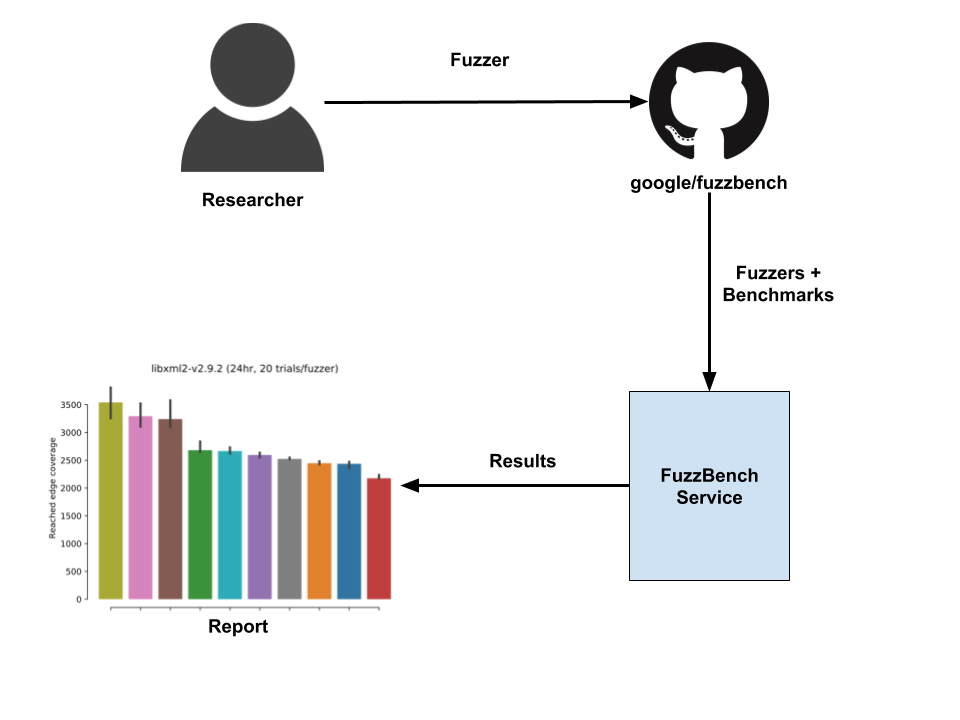
\includegraphics[width=\textwidth]{Chapter4/FuzzBench-service.png}
    \centering
    \caption{Fuzzbench overview}
    \label{fig:fuzzbench}
\end{figure}

Fuzzbench provides different modules for customized fuzzers. As illustrated in \ref{fig:fuzzbench}, we first introduce Waffle to fuzzbench by adding a directory of \texttt{Dockerfile}s, with the recipes for building and running the fuzz testing. Next, by passing the name of the fuzzers and the benchmarks, the evaluations begin to run as prescribed (3 trials, 12 hours). On the termination of all experiments, fuzzbench aggregates the performance of the fuzzers and benchmarks, and generates a comparative report of the whole benchmarking, and ranks the fuzzers based on their performance. Hence, the execution times are processed seperately for the execution time feature. In order to understand the whole procedure of testing, we explain how we have added Waffle to the system, and continue with the steps taken to get the results.

% -T: Explain the setup

\subsubsection{Add Waffle to FuzzBench}

\begin{sloppypar}
The current version of FuzzBench contains more than 30 different fuzzers available for testing. To evaluate Waffle, we need to first add Waffle to the list of known fuzzers which Fuzzbench communicates with. One of the options for adding a new fuzzer is by building a docker image, which builds Waffle project and passes \texttt{waffle-clang} compiler to fuzzbench for generating the binaries of the benchmarks. To build such docker images, we include the following files into \texttt{<fuzzbench-root>/fuzzers/waffle}:
\end{sloppypar}

\begin{itemize}
    \begin{sloppypar}
    \item \texttt{builder.Dockerfile:} This file builds the fuzzer in a docker container. Fuzzbench clones Waffle's project into the container, builds the project, and specifies a driver to provide the logs of the executions for fuzzbench. The recipe can be found in Appendix \ref{app:builder.docker}.
    \end{sloppypar}
    \item \texttt{runner.Dockerfile:} This file introduces compilation procedure for generating an instrumented binary of the target program. As Waffle is extending AFL, fuzzbench follows the same recipe, and generates the target file with the introduced (Waffle's) compiler.
    
    \item \texttt{fuzzer.py:} When fuzzbench finishes its setup for running a test, the content of \texttt{fuzzer.py} executes fuzz testing without showing the status screen, and creates running instances of the trials. [Appendix \ref{app:fuzzer.py}].
\end{itemize}

\subsubsection{Start an experiment}

We use a \textbf{local experiment} for evaluations. The local computer runs on Ubuntu 18.04 64bits, with Intel® Core™ i7-3770 CPU @ 3.40GHz × 8, and 16 GBs of RAM. The measurements for the performance of HDD, show 30MB/s for reading from the disk, and can write for 25MB/s.

\section{Evaluation metrics}
\label{sec:ch4-metrics}

% -T: Define the metrics: code coverage

Fuzzbench implements a Clang-based fuzzer-independent code coverage measurer, which calculates the code coverage of the benchmarks after completion of each trial. Same as mentioned in AFL's code coverage measurement, the taken edges exhibit the covered regions in an execution. Table \ref{table:benchmarks} shows the benchmarks used in our tests (within fuzzbench); the last column of the table shows the total number of edges for each of the benchmarks. Other columns indicate if the provided benchmark is supported by a dictionary for the syntax of the inputs, the format of the inputs, and the number of provided seeds for fuzzing the programs. 

\begin{table}[]
    \centering
    \resizebox{\textwidth}{!}{
    \begin{tabular}{|c|c|c|c|c|}
    \hline
    \rowcolor{lightgray}
    Benchmark             & Dictionary & Format         & Seeds & Edges \\
    \hline
    freetype2-2017        & \xmark     & TTF, OTF, WOFF & 2     & 19056 \\
    \hline q
    libjpeg-turbo-07-2017 & \xmark     & JPEG           & 1     & 9586  \\
    \hline
    libpng-1.2.56         & \cmark     & PNG            & 1     & 2991  \\
    \hline
    libxml2-v2.9.2        & \cmark     & XML            & 0     & 50461 \\
    \hline    
    \end{tabular}%
    }
    \caption{List of benchmarks used in evaluation}
    \label{table:benchmarks}
\end{table}

% -T: Define the metrics: execution time, and explain how we collect it

The main metric for fuzzbench's comparisons is the code coverage, but as we intended to evaluate the execution times as well, we developed a post-processing module for checking the execution times of the generated entries of the trials of fuzzbench. Benchmarks are built within fuzzbench Docker containers, and instead of rebuilding the benchmarks separately, we investigate the execution times within the container with an uninstrumented binary of the target. The measurement of the execution times is implemented in Python 3. The execution times are measured by running the target program with each of the queue entries 10 times, and we assigned the average of the values as the execution time on the provided input.

\section{Evaluation results}
\label{sec:ch4-report}

The report generated by fuzzbench collecting the coverage information is placed in \texttt{report-data} directory, beside the experiment files located in \texttt{xp-data}. The reports are generated in figures and an HTML file for illustrating the results. We first analyze the code coverages, and then we examine the execution times.

\subsection{Code coverage}

\subsubsection{Code coverage growth}

Figure \ref{fig:cov-growth} shows the code coverage growth of the fuzzers, while fuzzing each benchmark. There are three trials for each fuzzer, and the illustration shows the highest code coverage, the minimum code coverage, and the median of the trials' results. AFL++ shows a significant better performance than other benchmarks. In fact, AFL++ is has the highest performance in coverage among all other benchmarks which are provided in fuzzbench project. Waffle, as expected, is seemingly performing same as AFL. This is followed by the fact that Waffle performs the same code coverage approach, but there are new different features for producing queue entries. In \ref{fig:sub:freetype-cov-growth}, the trials of Waffle show more variance in performance. Hence, AFL's trials grow close to each other. In the paper based on fuzzbench results \cite{metzman2021fuzzbench}, the \texttt{deterministic stages} of AFL's fuzzing is behind such performance. It is also noticeable that Waffle discovers significantly more regions in at least one of the trials. Testing libjpeg-turbo-07-2017 (Figure \ref{fig:sub:libjpeg-cov-growth}) and libpng-1.2.56 (Figure \ref{fig:sub:libpng-cov-growth}) show a close performance for AFL, AFLFast, and Waffle \ref{fig:sub:libjpeg-cov-growth}. Another interesting result collected from fuzzing libxml2-v2.9.2 suggests a difficulty for Waffle in exploring the code coverage, but eventually Waffle gets the pace closer to other fuzzers. In addition, AFL is the winner of the 4th experiment.

\begin{figure}
    \centering
    \begin{subfigure}[t]{\textwidth}
        \centering
        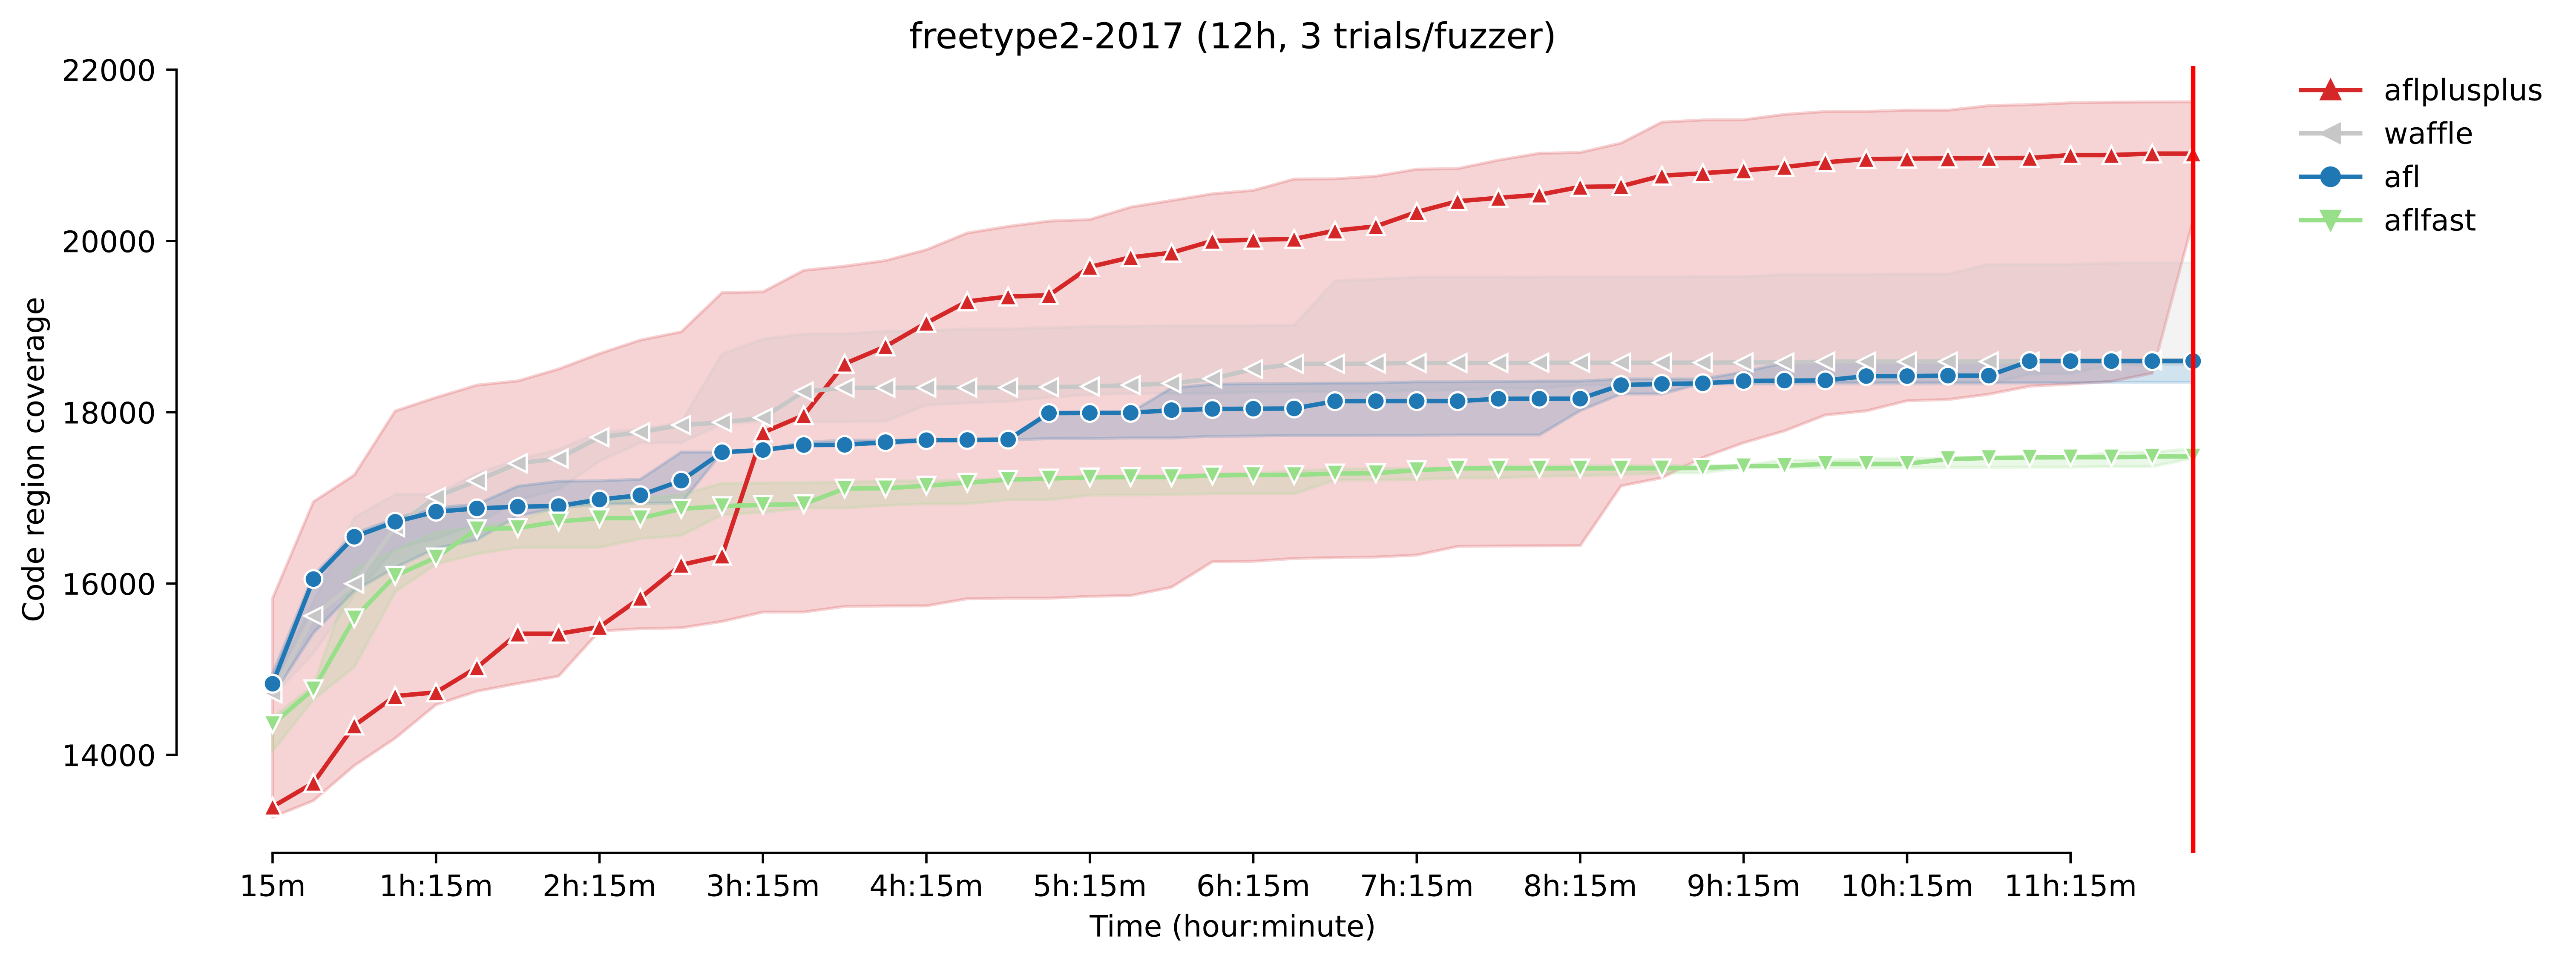
\includegraphics[width=0.85\textwidth]{Experiments/freetype2-2017_coverage_growth.png}
        \caption{freetype2-2017}
        \label{fig:sub:freetype-cov-growth}
    \end{subfigure}

    \begin{subfigure}[t]{\textwidth}
        \centering
        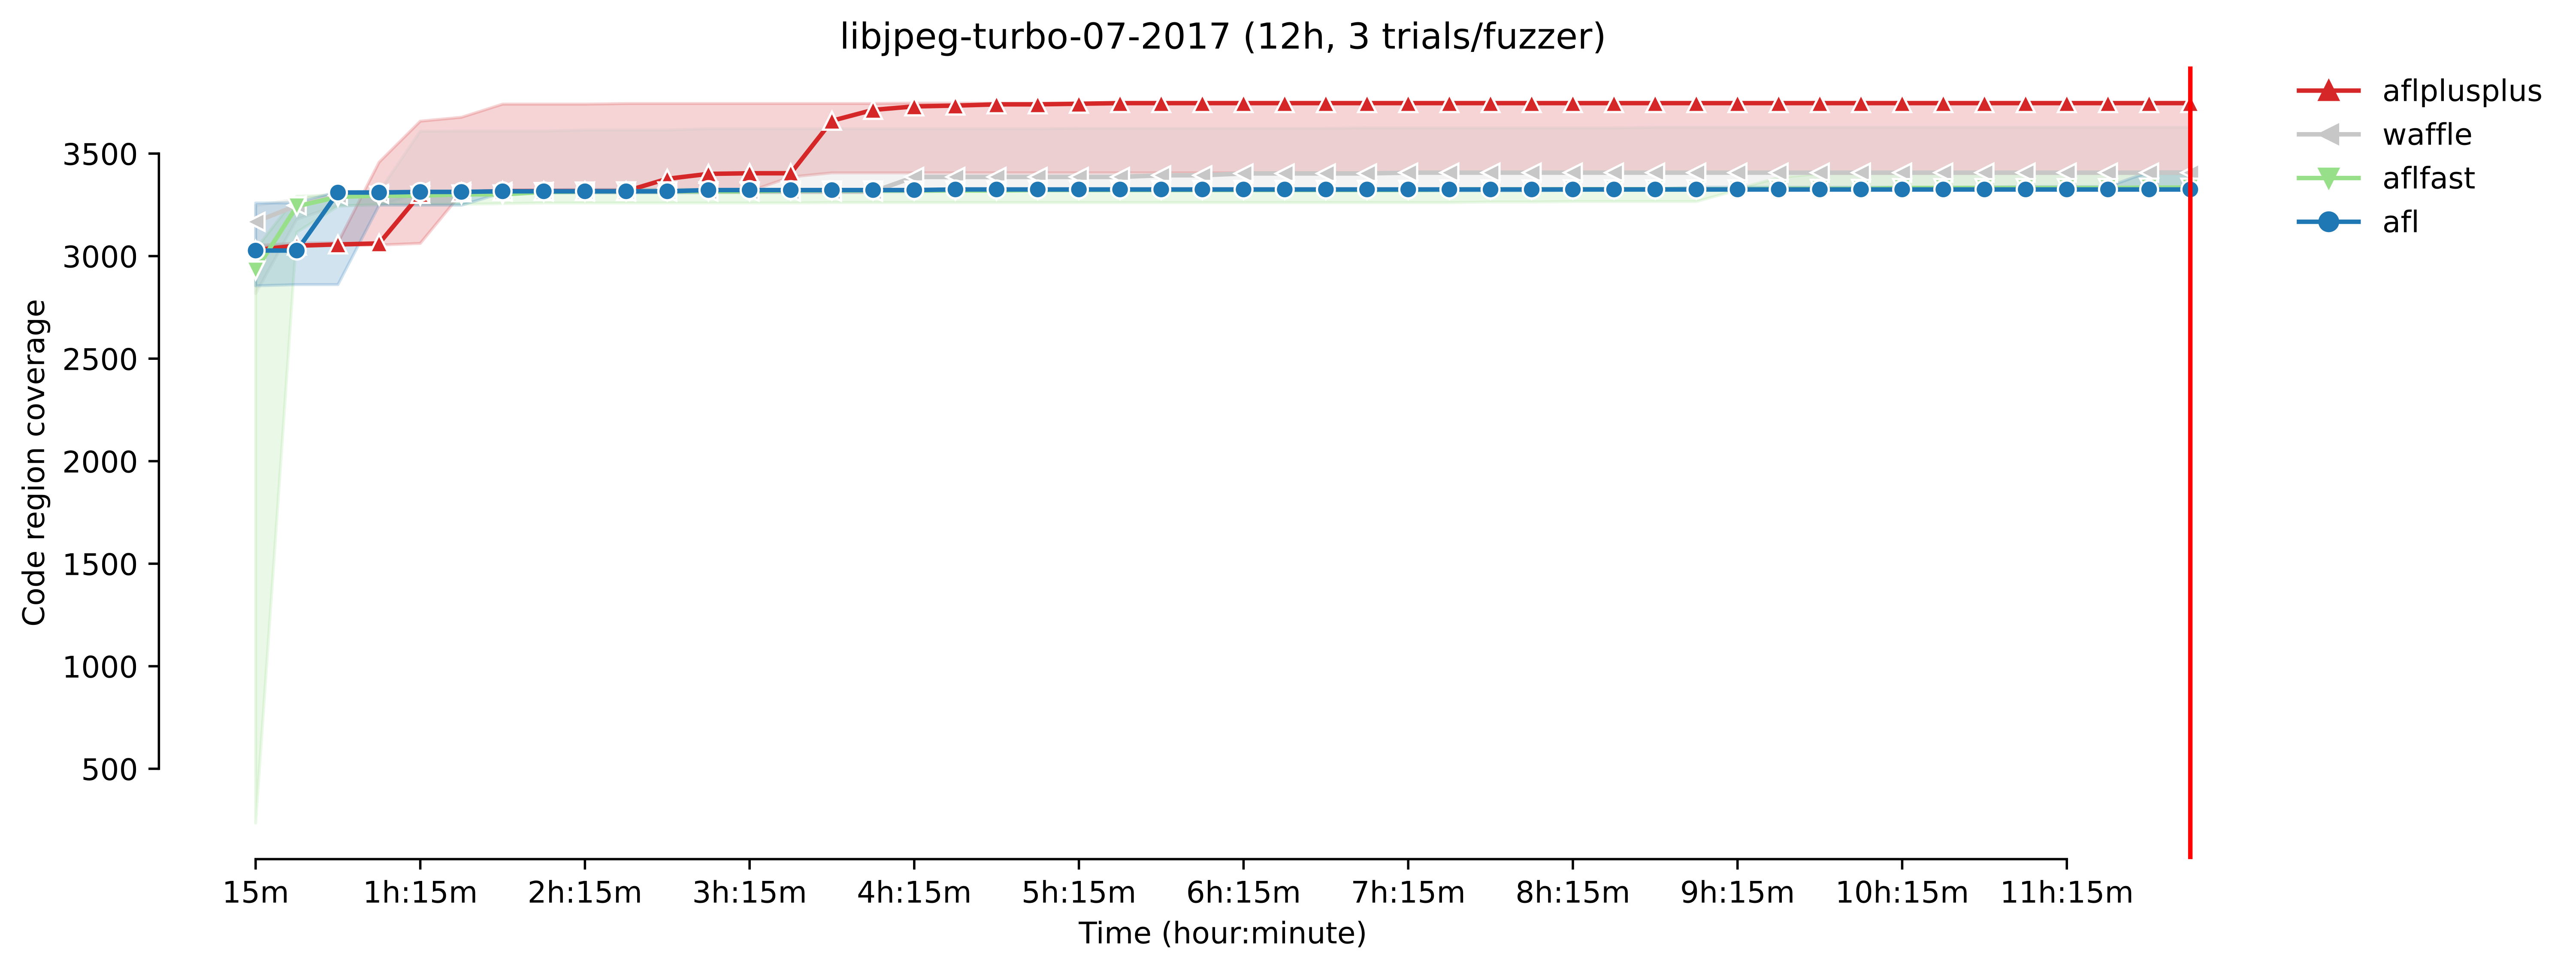
\includegraphics[width=0.85\textwidth]{Experiments/libjpeg-turbo-07-2017_coverage_growth.png}
        \caption{libjpeg-turbo-07-2017}
        \label{fig:sub:libjpeg-cov-growth}
    \end{subfigure}

    \begin{subfigure}[t]{\textwidth}
        \centering
        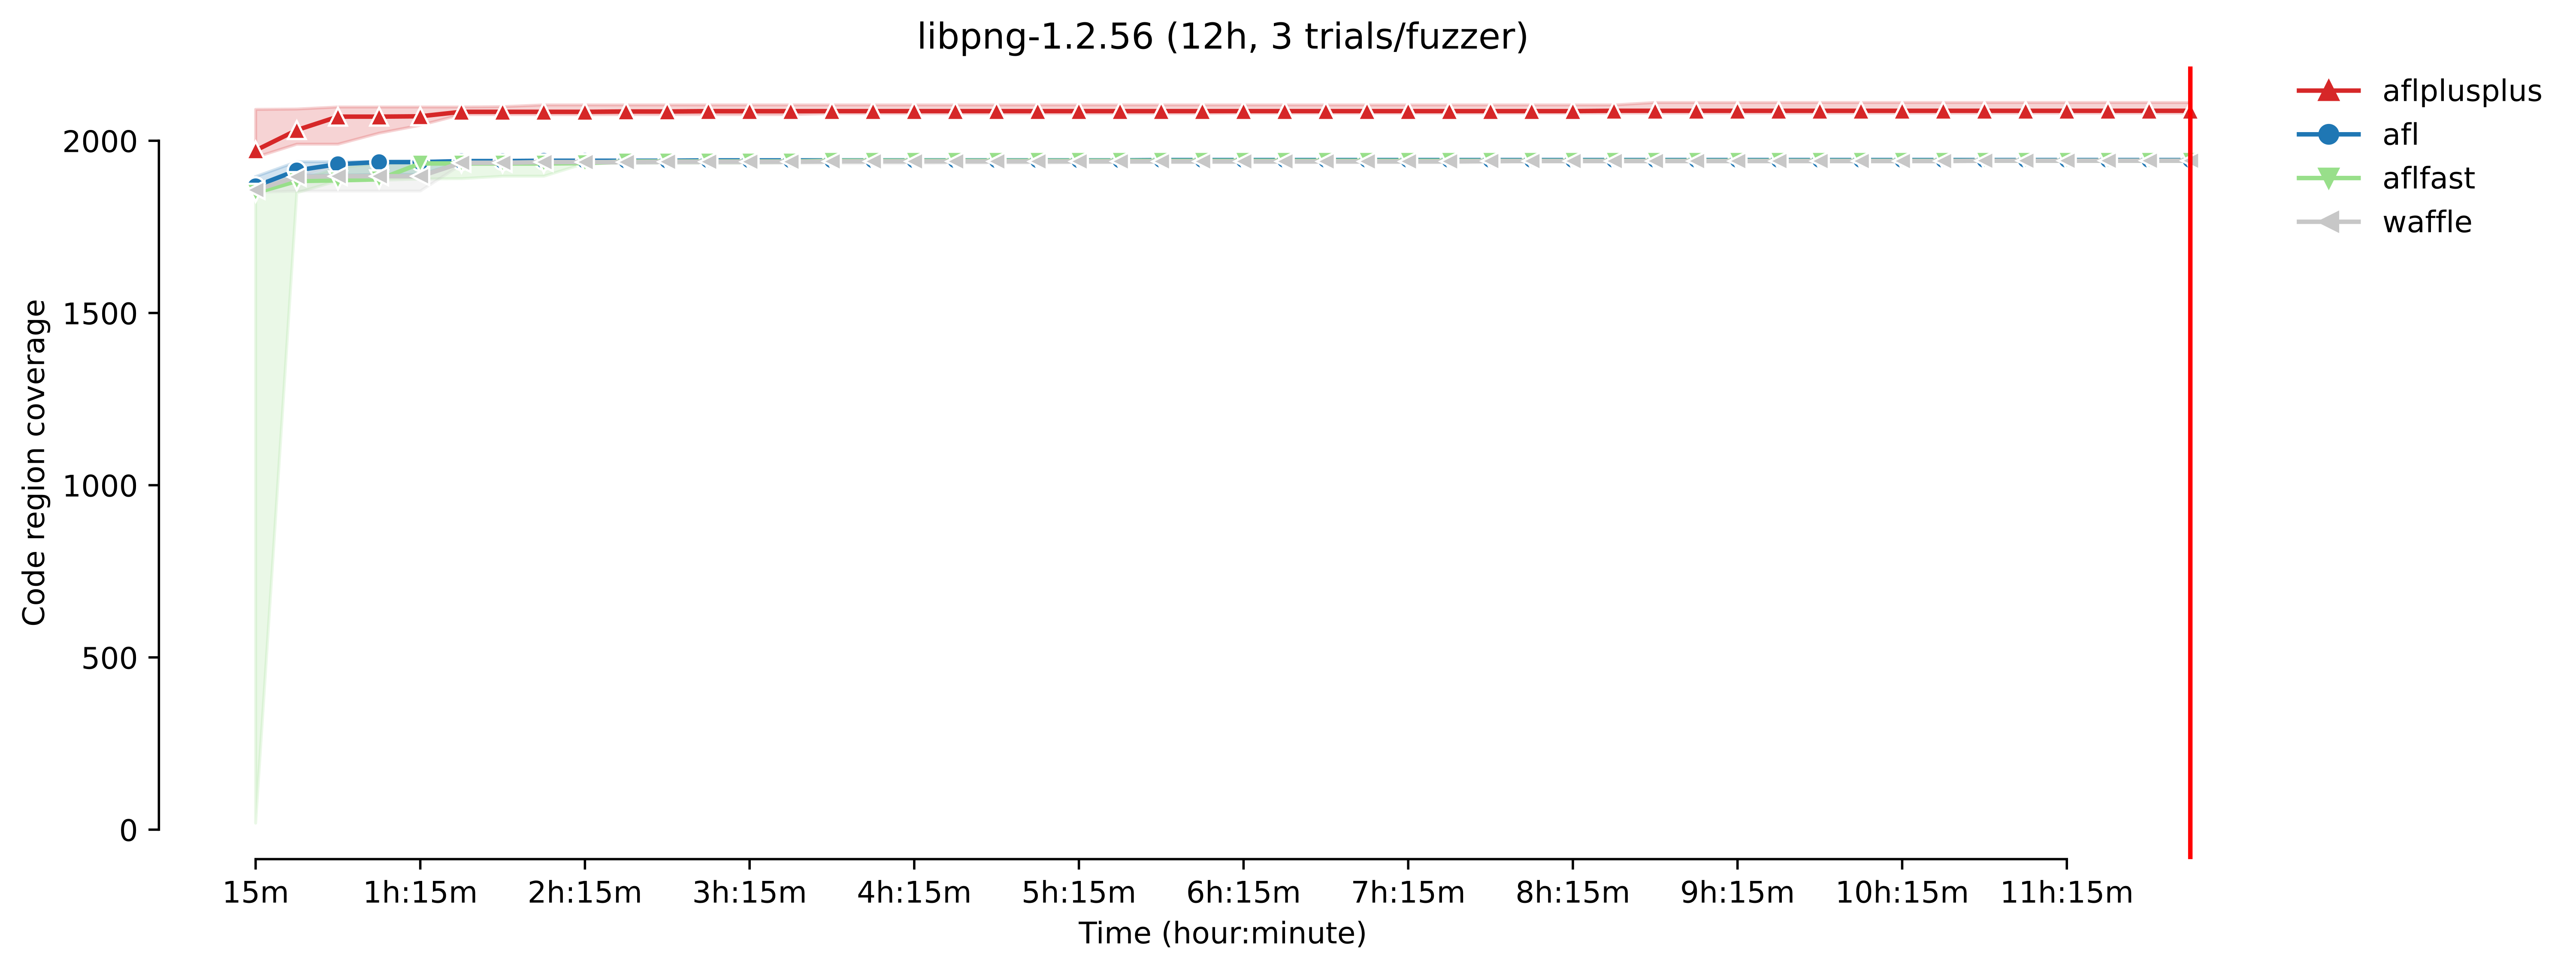
\includegraphics[width=0.85\textwidth]{Experiments/libpng-1.2.56_coverage_growth.png}
        \caption{libpng-1.2.56}
        \label{fig:sub:libpng-cov-growth}
    \end{subfigure}

    \begin{subfigure}[t]{\textwidth}
        \centering
        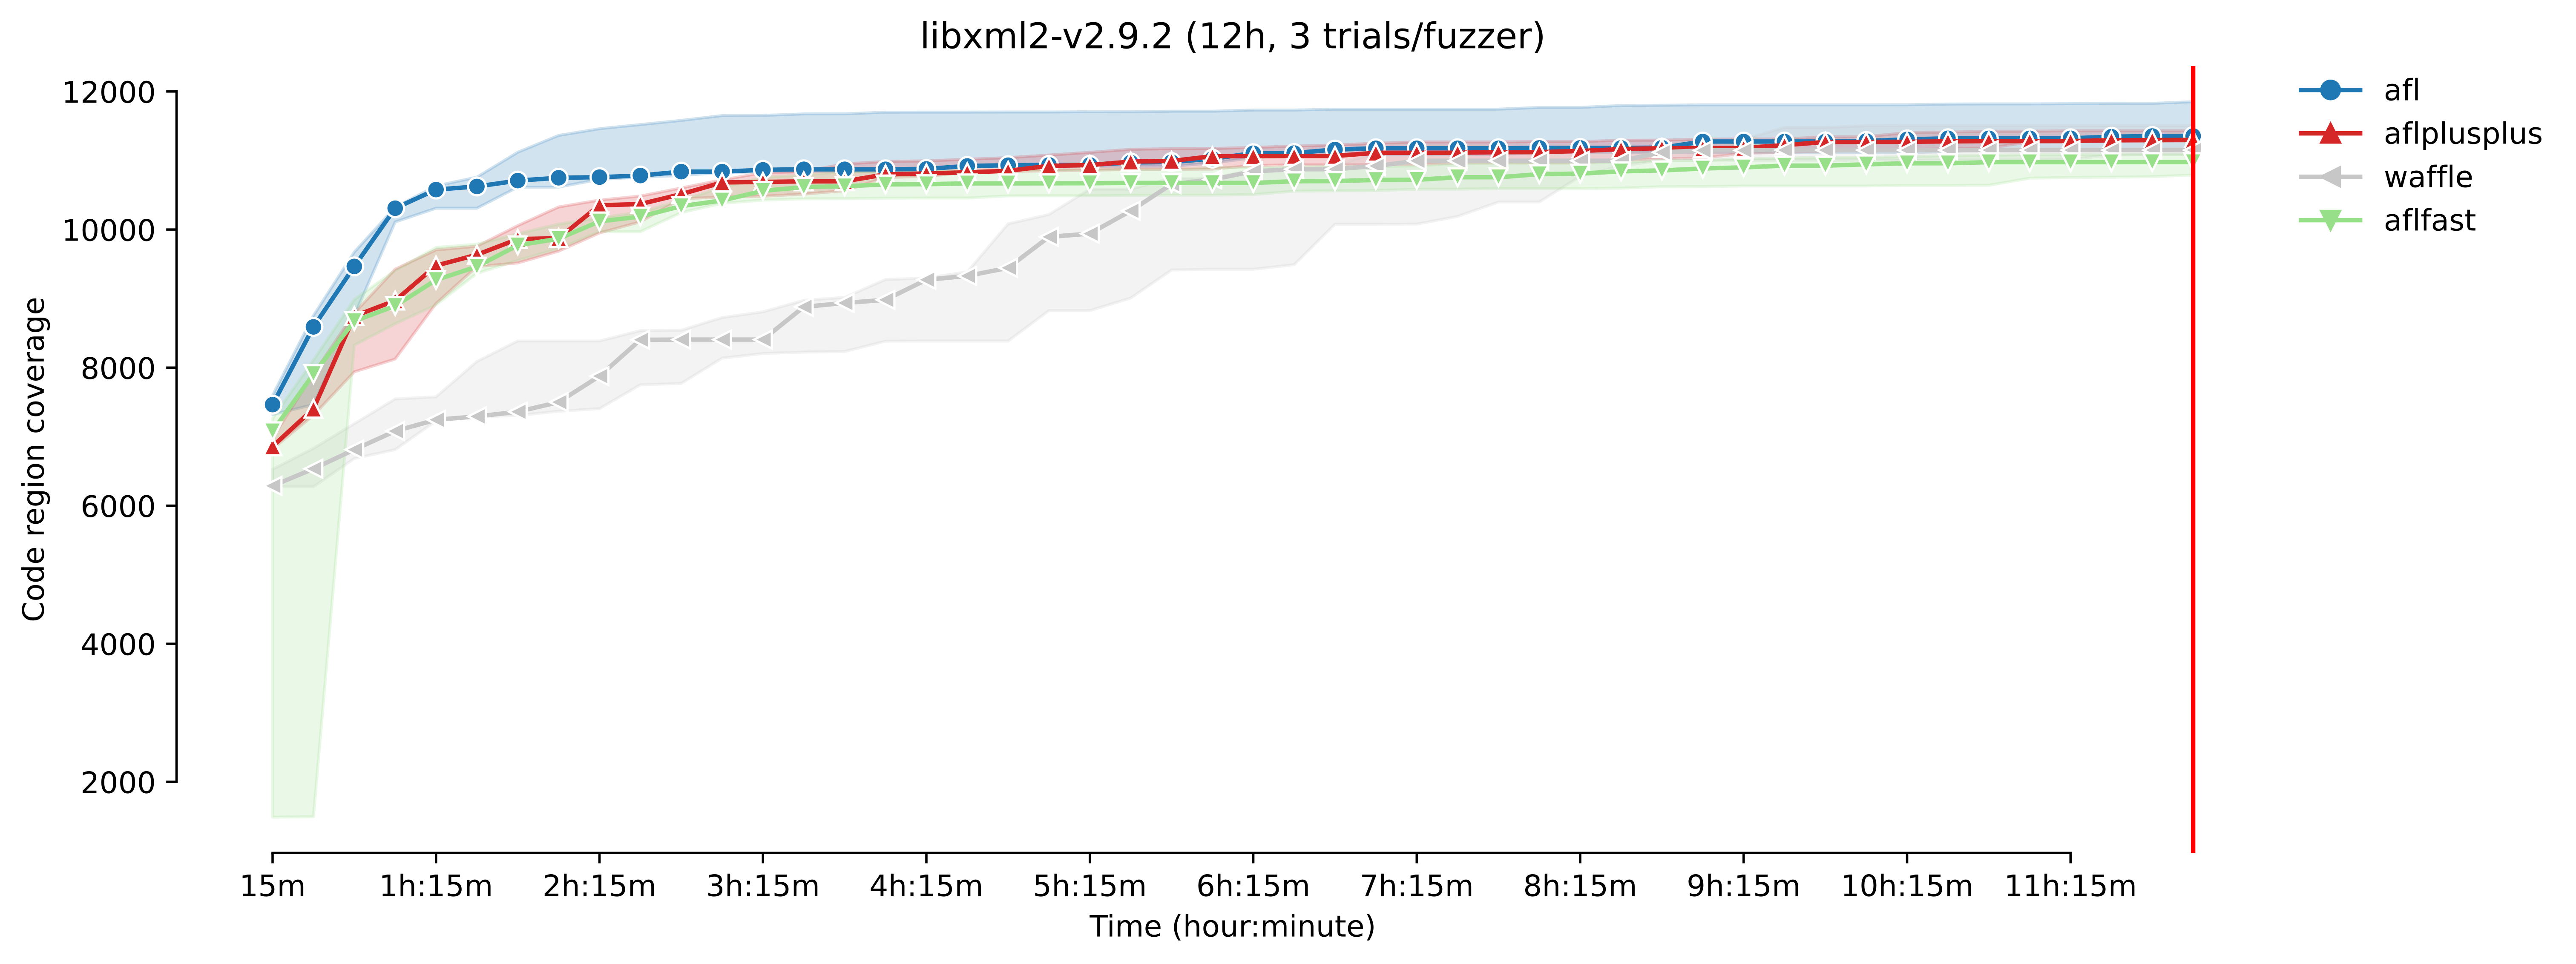
\includegraphics[width=0.85\textwidth]{Experiments/libxml2-v2.9.2_coverage_growth.png}
        \caption{libxml2-v2.9.2}
        \label{fig:sub:libxml-cov-growth}
    \end{subfigure}

    \caption{Coverage growth during the trials}
    \label{fig:cov-growth}
\end{figure}

\subsubsection{Unique code coverage findings}

Based on the results collected after each trial, fuzzbench also measures the uniqueness of the fuzzer's findings. Figure \ref{fig:cov-uniq} shows the number of code regions that were uniquely covered in a pairwise fashion. The coloring specifies the significance of the differences; the darker the color is, the more findings are uniquely found by the fuzzer on bottom.

% ! Should explain more?

\begin{figure}
    \centering
    \begin{subfigure}[t]{\textwidth}
        \centering
        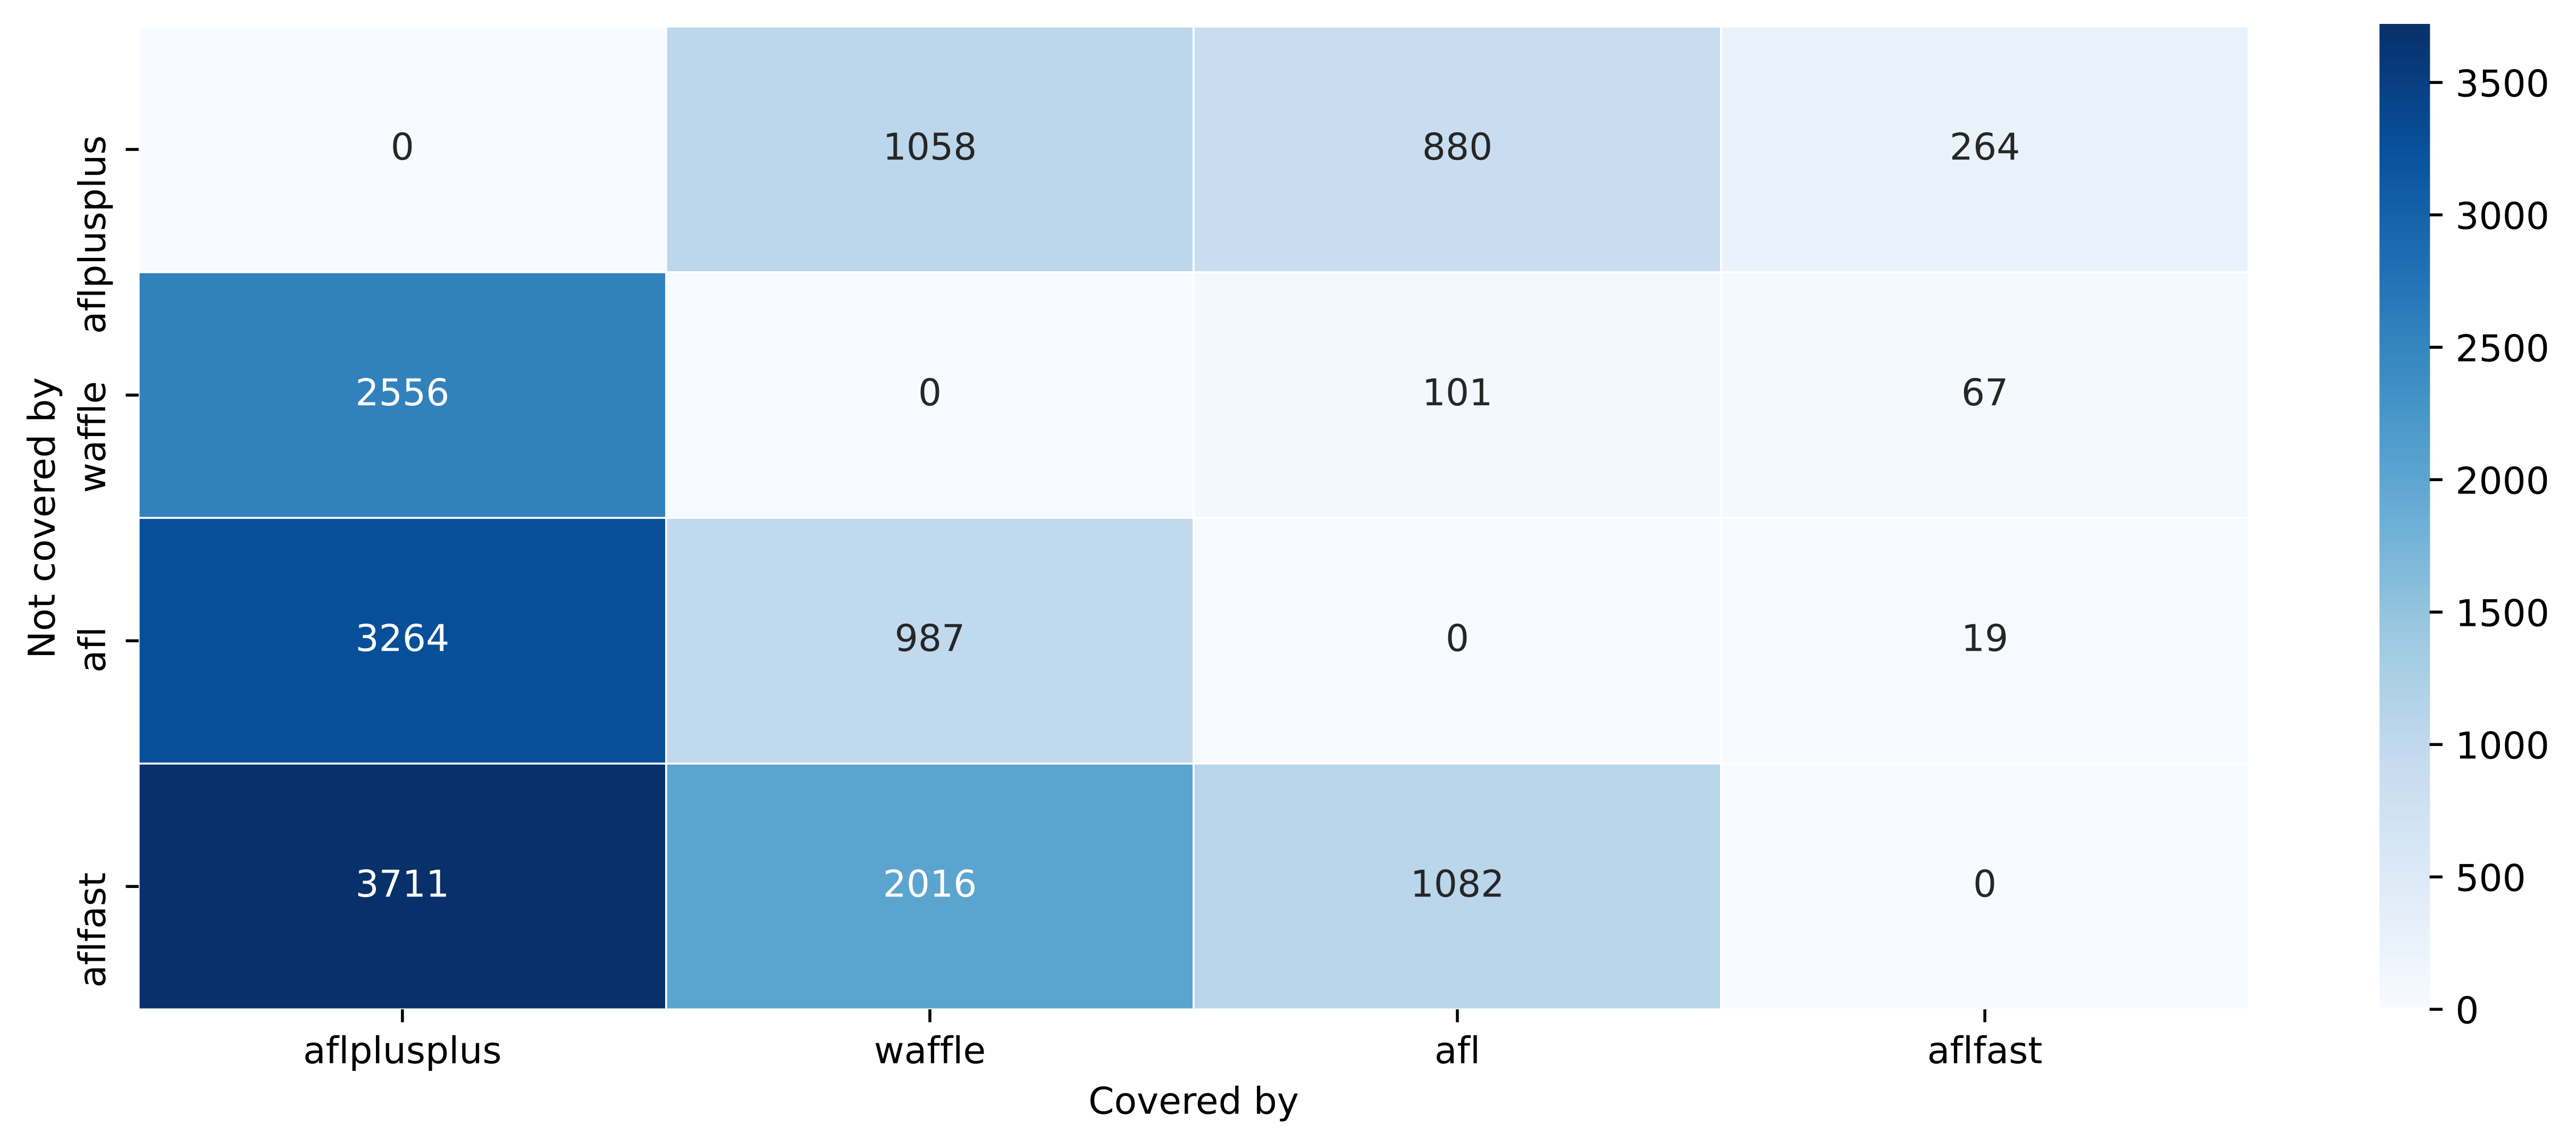
\includegraphics[width=0.70\textwidth]{Experiments/freetype2-2017_pairwise_unique_coverage_plot.png}
        \caption{freetype2-2017}
        \label{fig:sub:freetype-cov-uniq}
    \end{subfigure}

    \begin{subfigure}[t]{\textwidth}
        \centering
        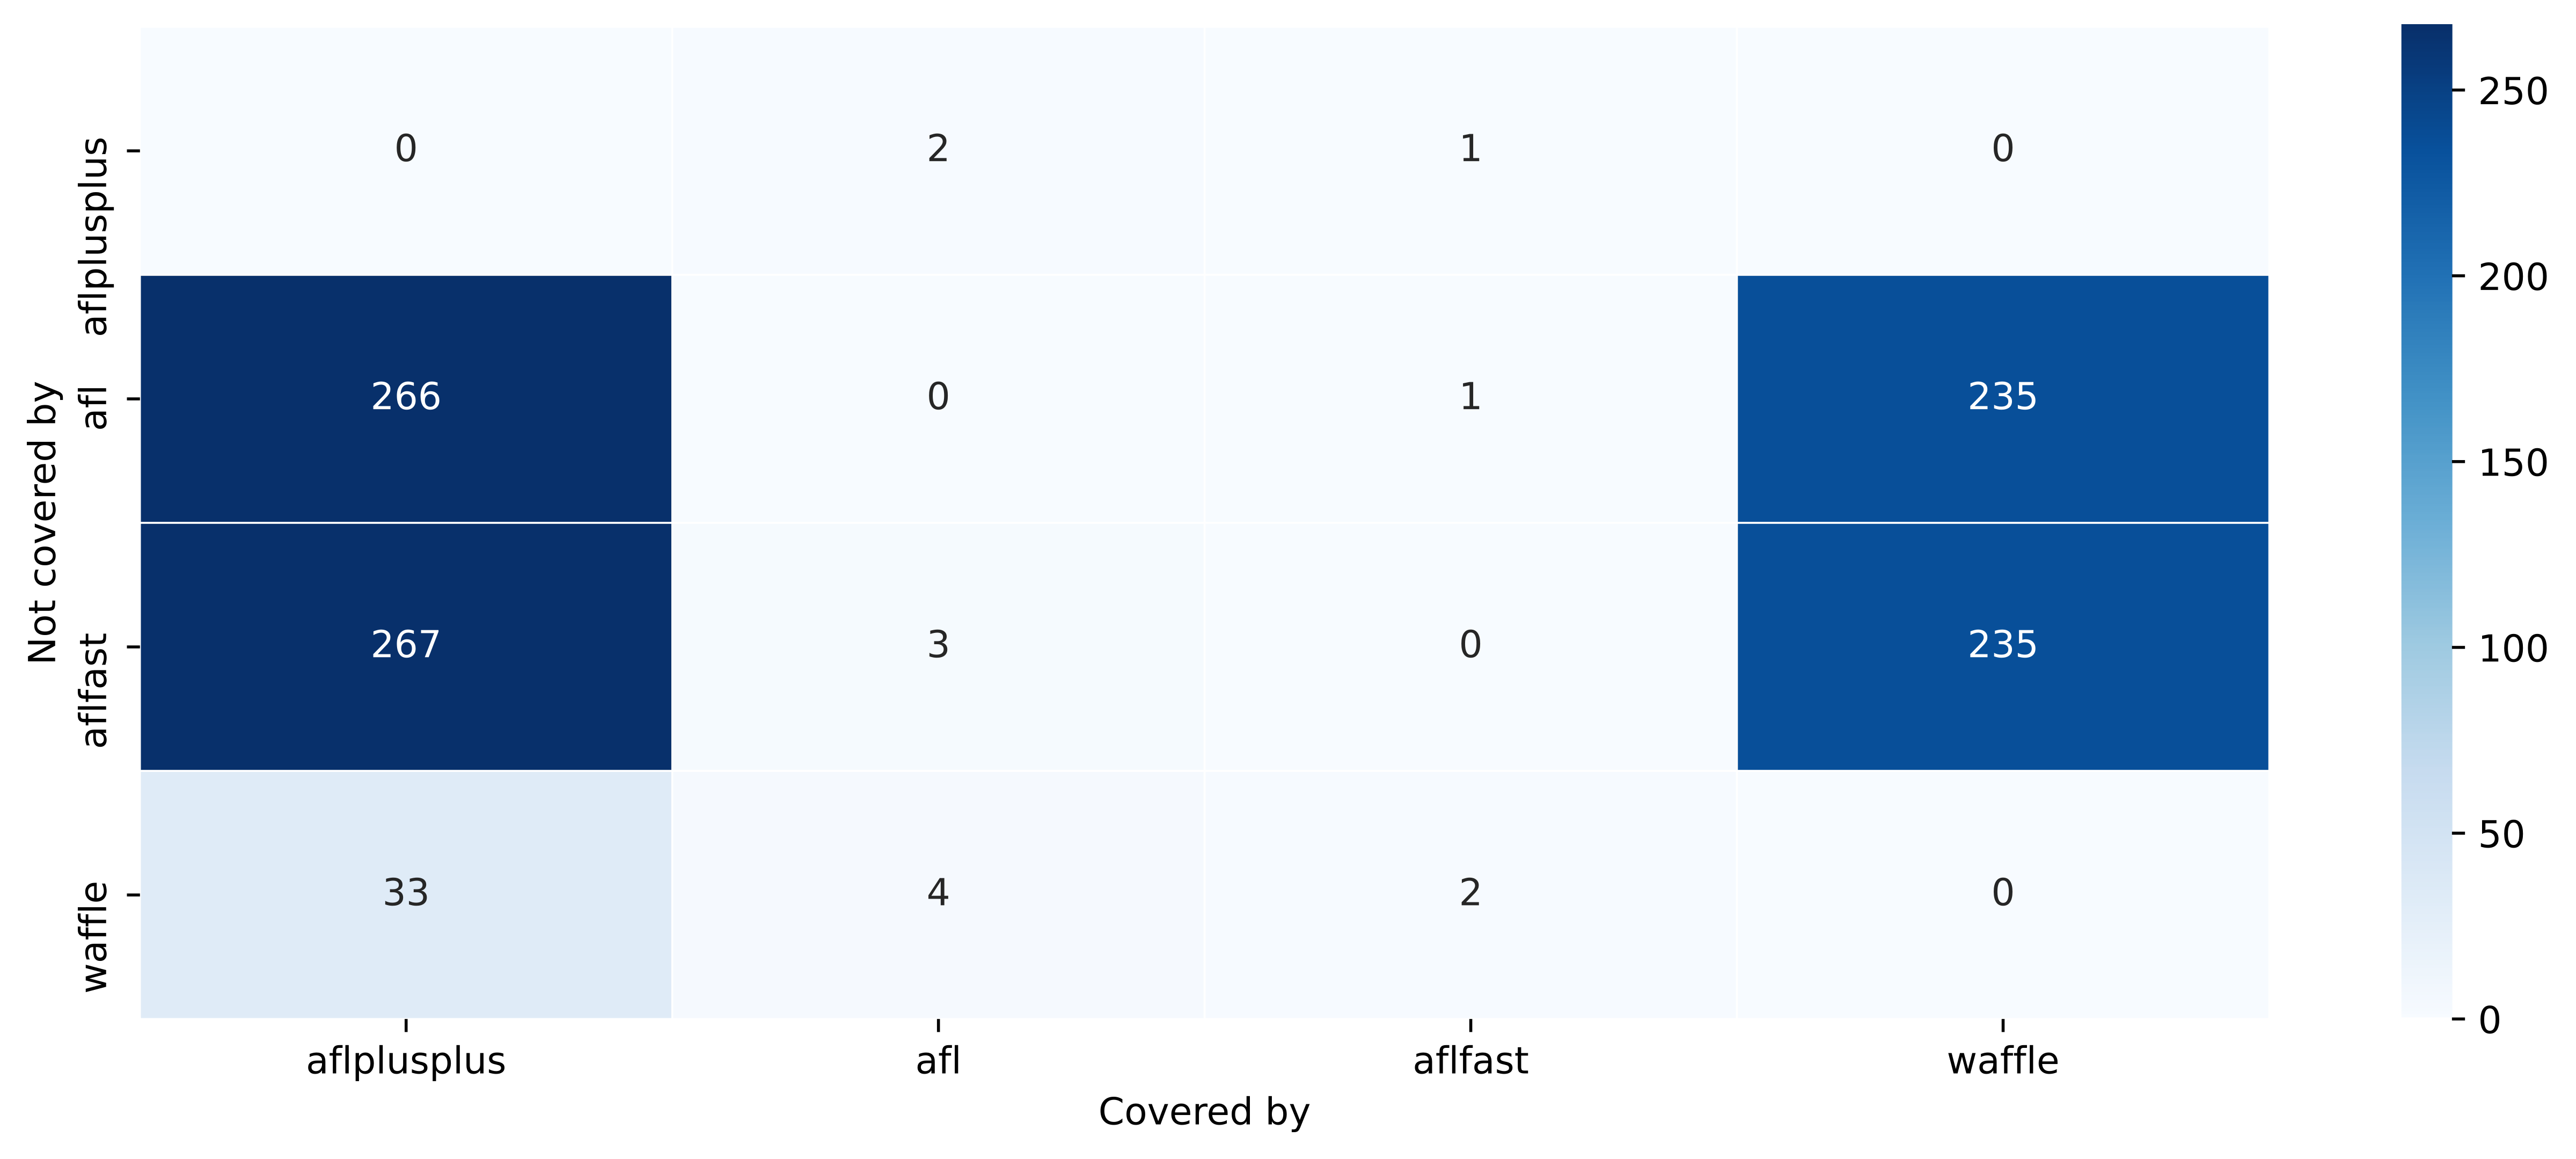
\includegraphics[width=0.70\textwidth]{Experiments/libjpeg-turbo-07-2017_pairwise_unique_coverage_plot.png}
        \caption{libjpeg-turbo-07-2017}
        \label{fig:sub:libjpeg-cov-uniq}
    \end{subfigure}

    \begin{subfigure}[t]{\textwidth}
        \centering
        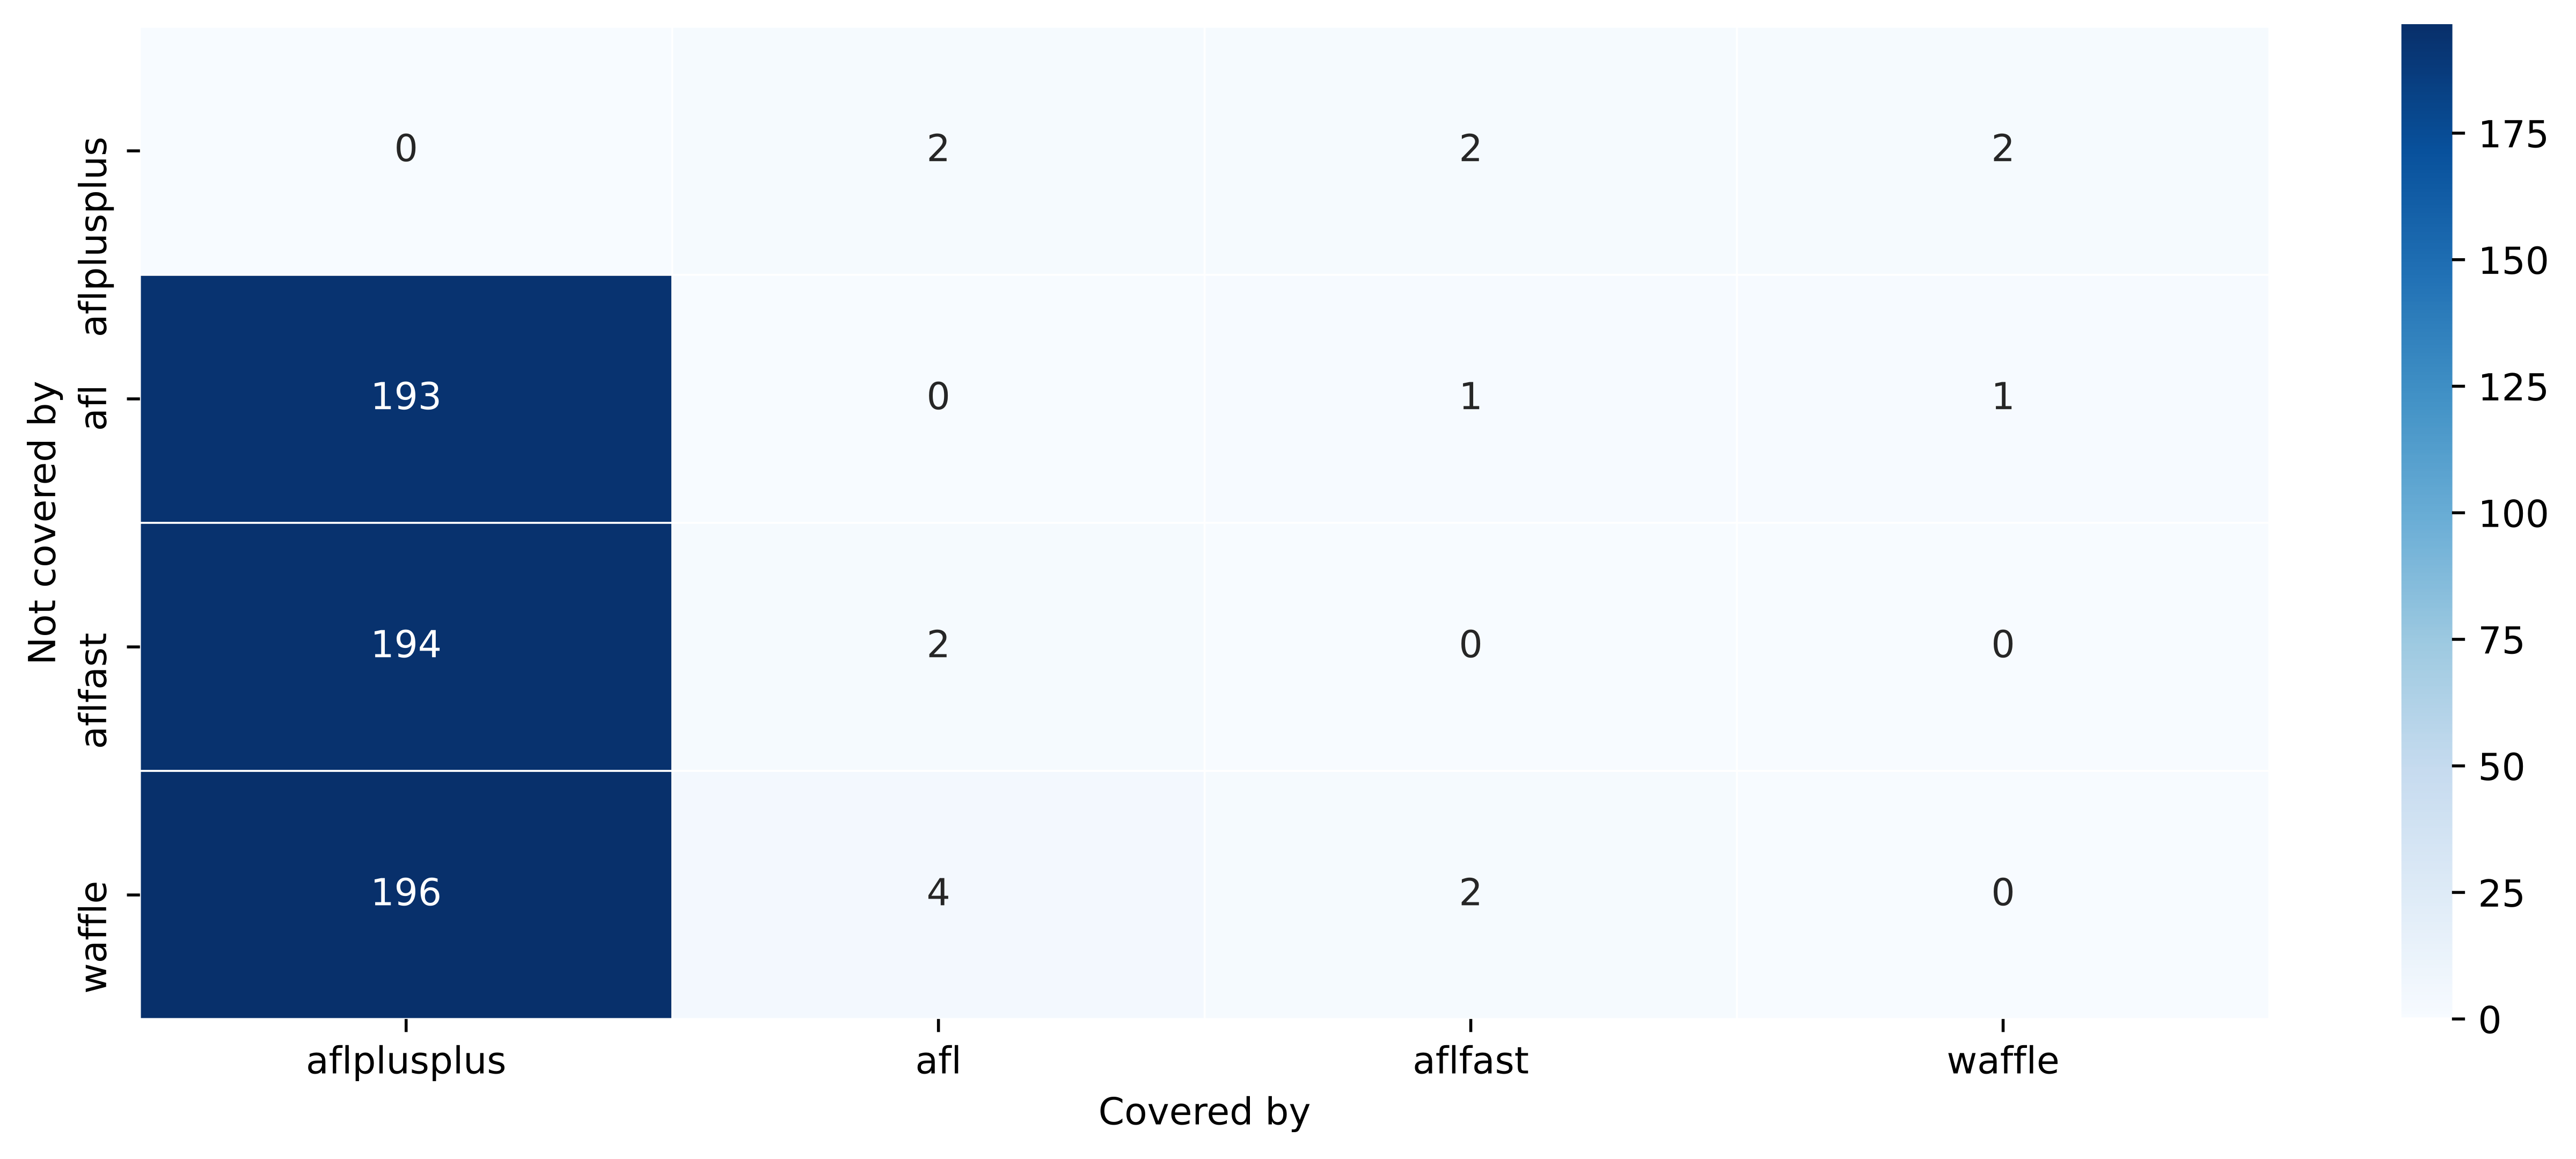
\includegraphics[width=0.70\textwidth]{Experiments/libpng-1.2.56_pairwise_unique_coverage_plot.png}
        \caption{libpng-1.2.56}
        \label{fig:sub:libpng-cov-uniq}
    \end{subfigure}

    \begin{subfigure}[t]{\textwidth}
        \centering
        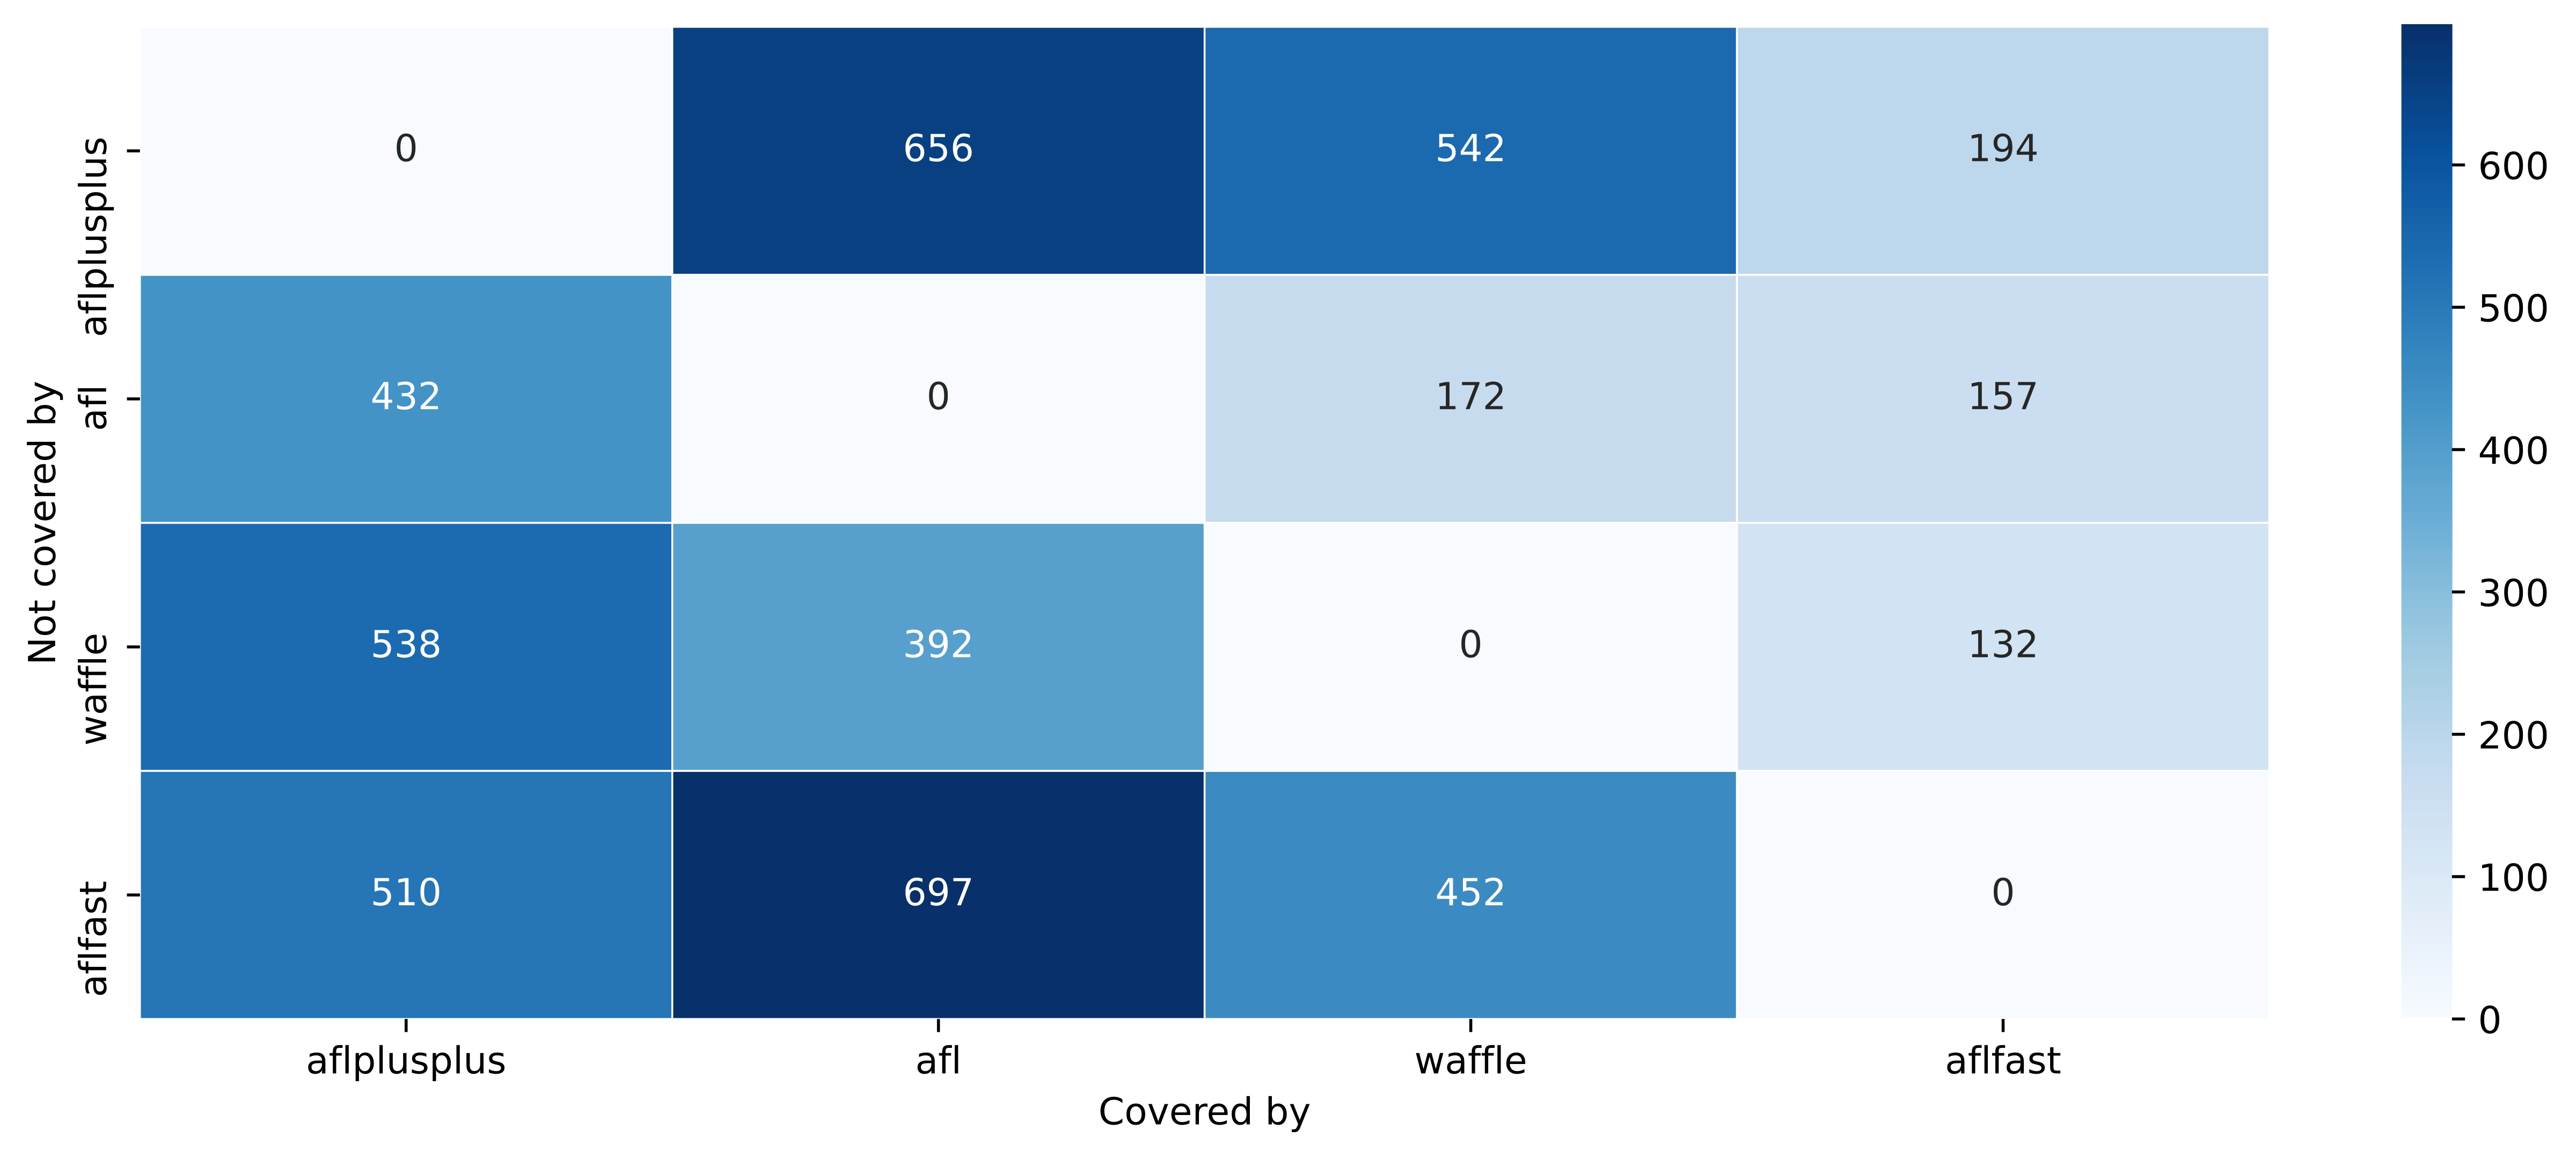
\includegraphics[width=0.70\textwidth]{Experiments/libxml2-v2.9.2_pairwise_unique_coverage_plot.png}
        \caption{libxml2-v2.9.2}
        \label{fig:sub:libxml-cov-uniq}
    \end{subfigure}

    \caption{Unique coverage findings}
    \label{fig:cov-uniq}
\end{figure}

% \subsubsection{Vargha-Delaney's A12 measurements}

% \begin{figure}
%     \centering
%     \begin{subfigure}[b]{0.475\linewidth}
%         \centering
%         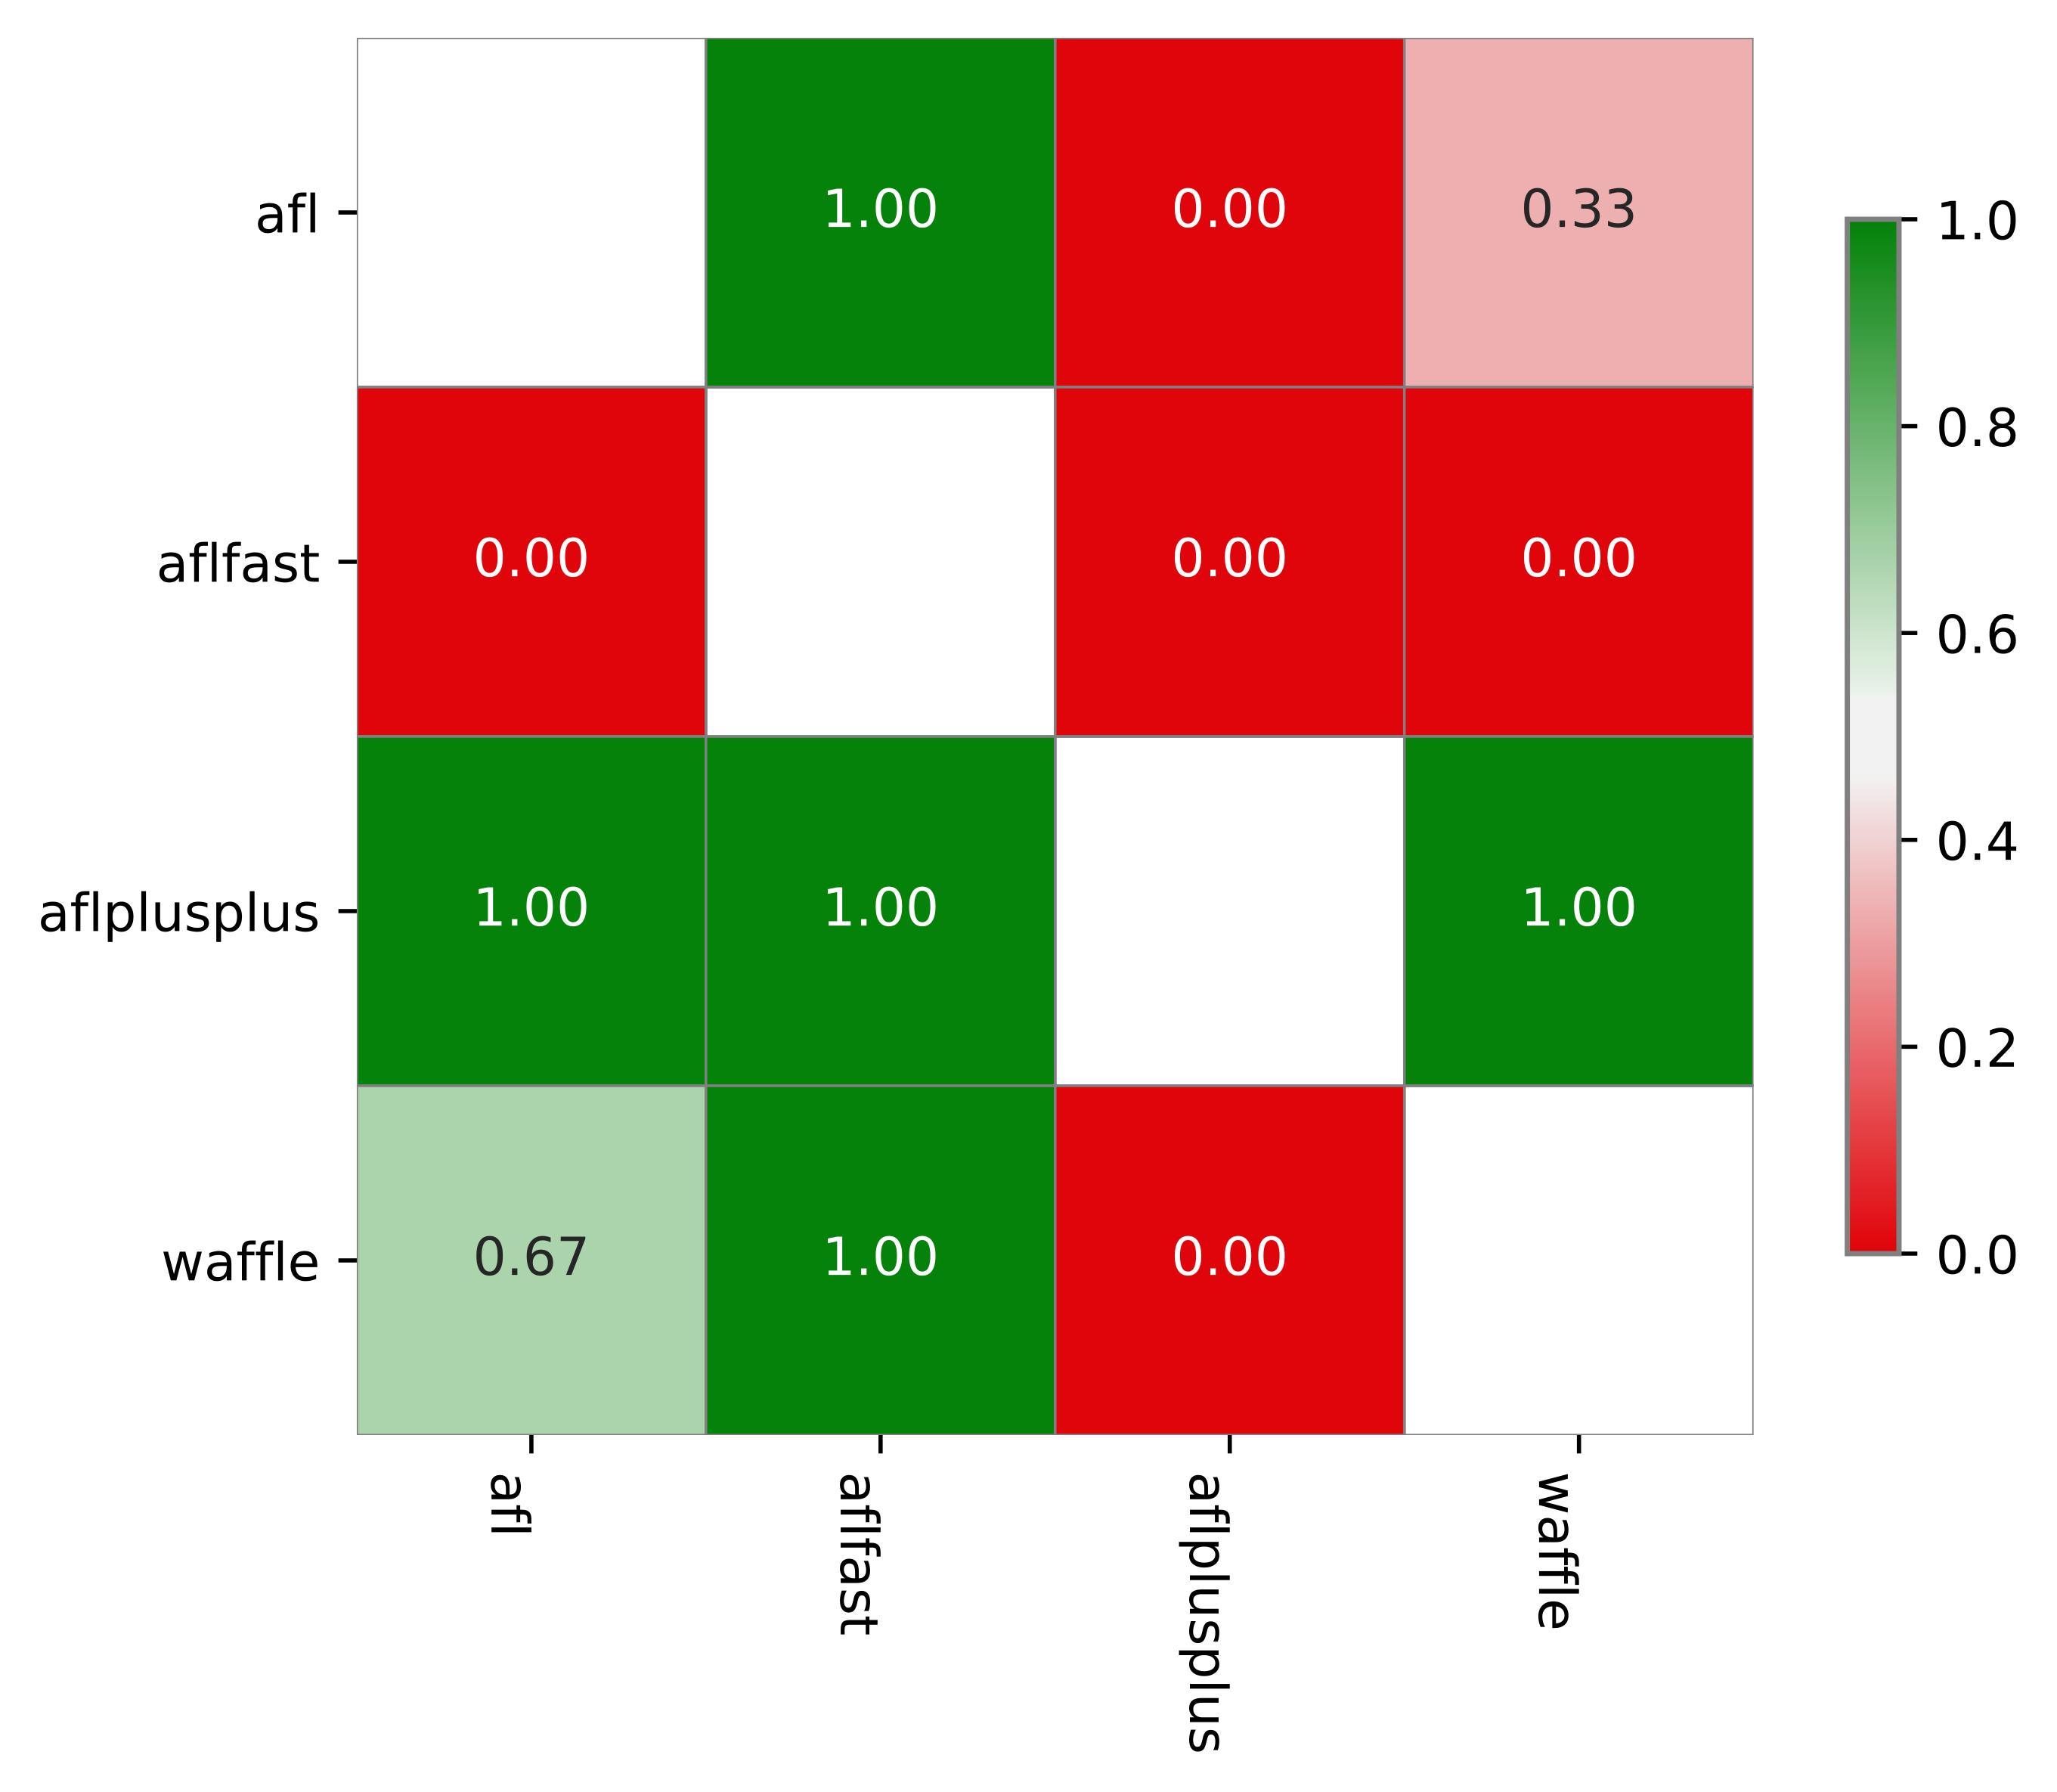
\includegraphics[width=0.95\linewidth]{Experiments/freetype2-2017_varga_delaney_a12_plot.png}
%         \caption{freetype2-2017}
%         \label{fig:sub:freetype-vda12}
%     \end{subfigure}
%     \begin{subfigure}[b]{0.475\linewidth}
%         \centering
%         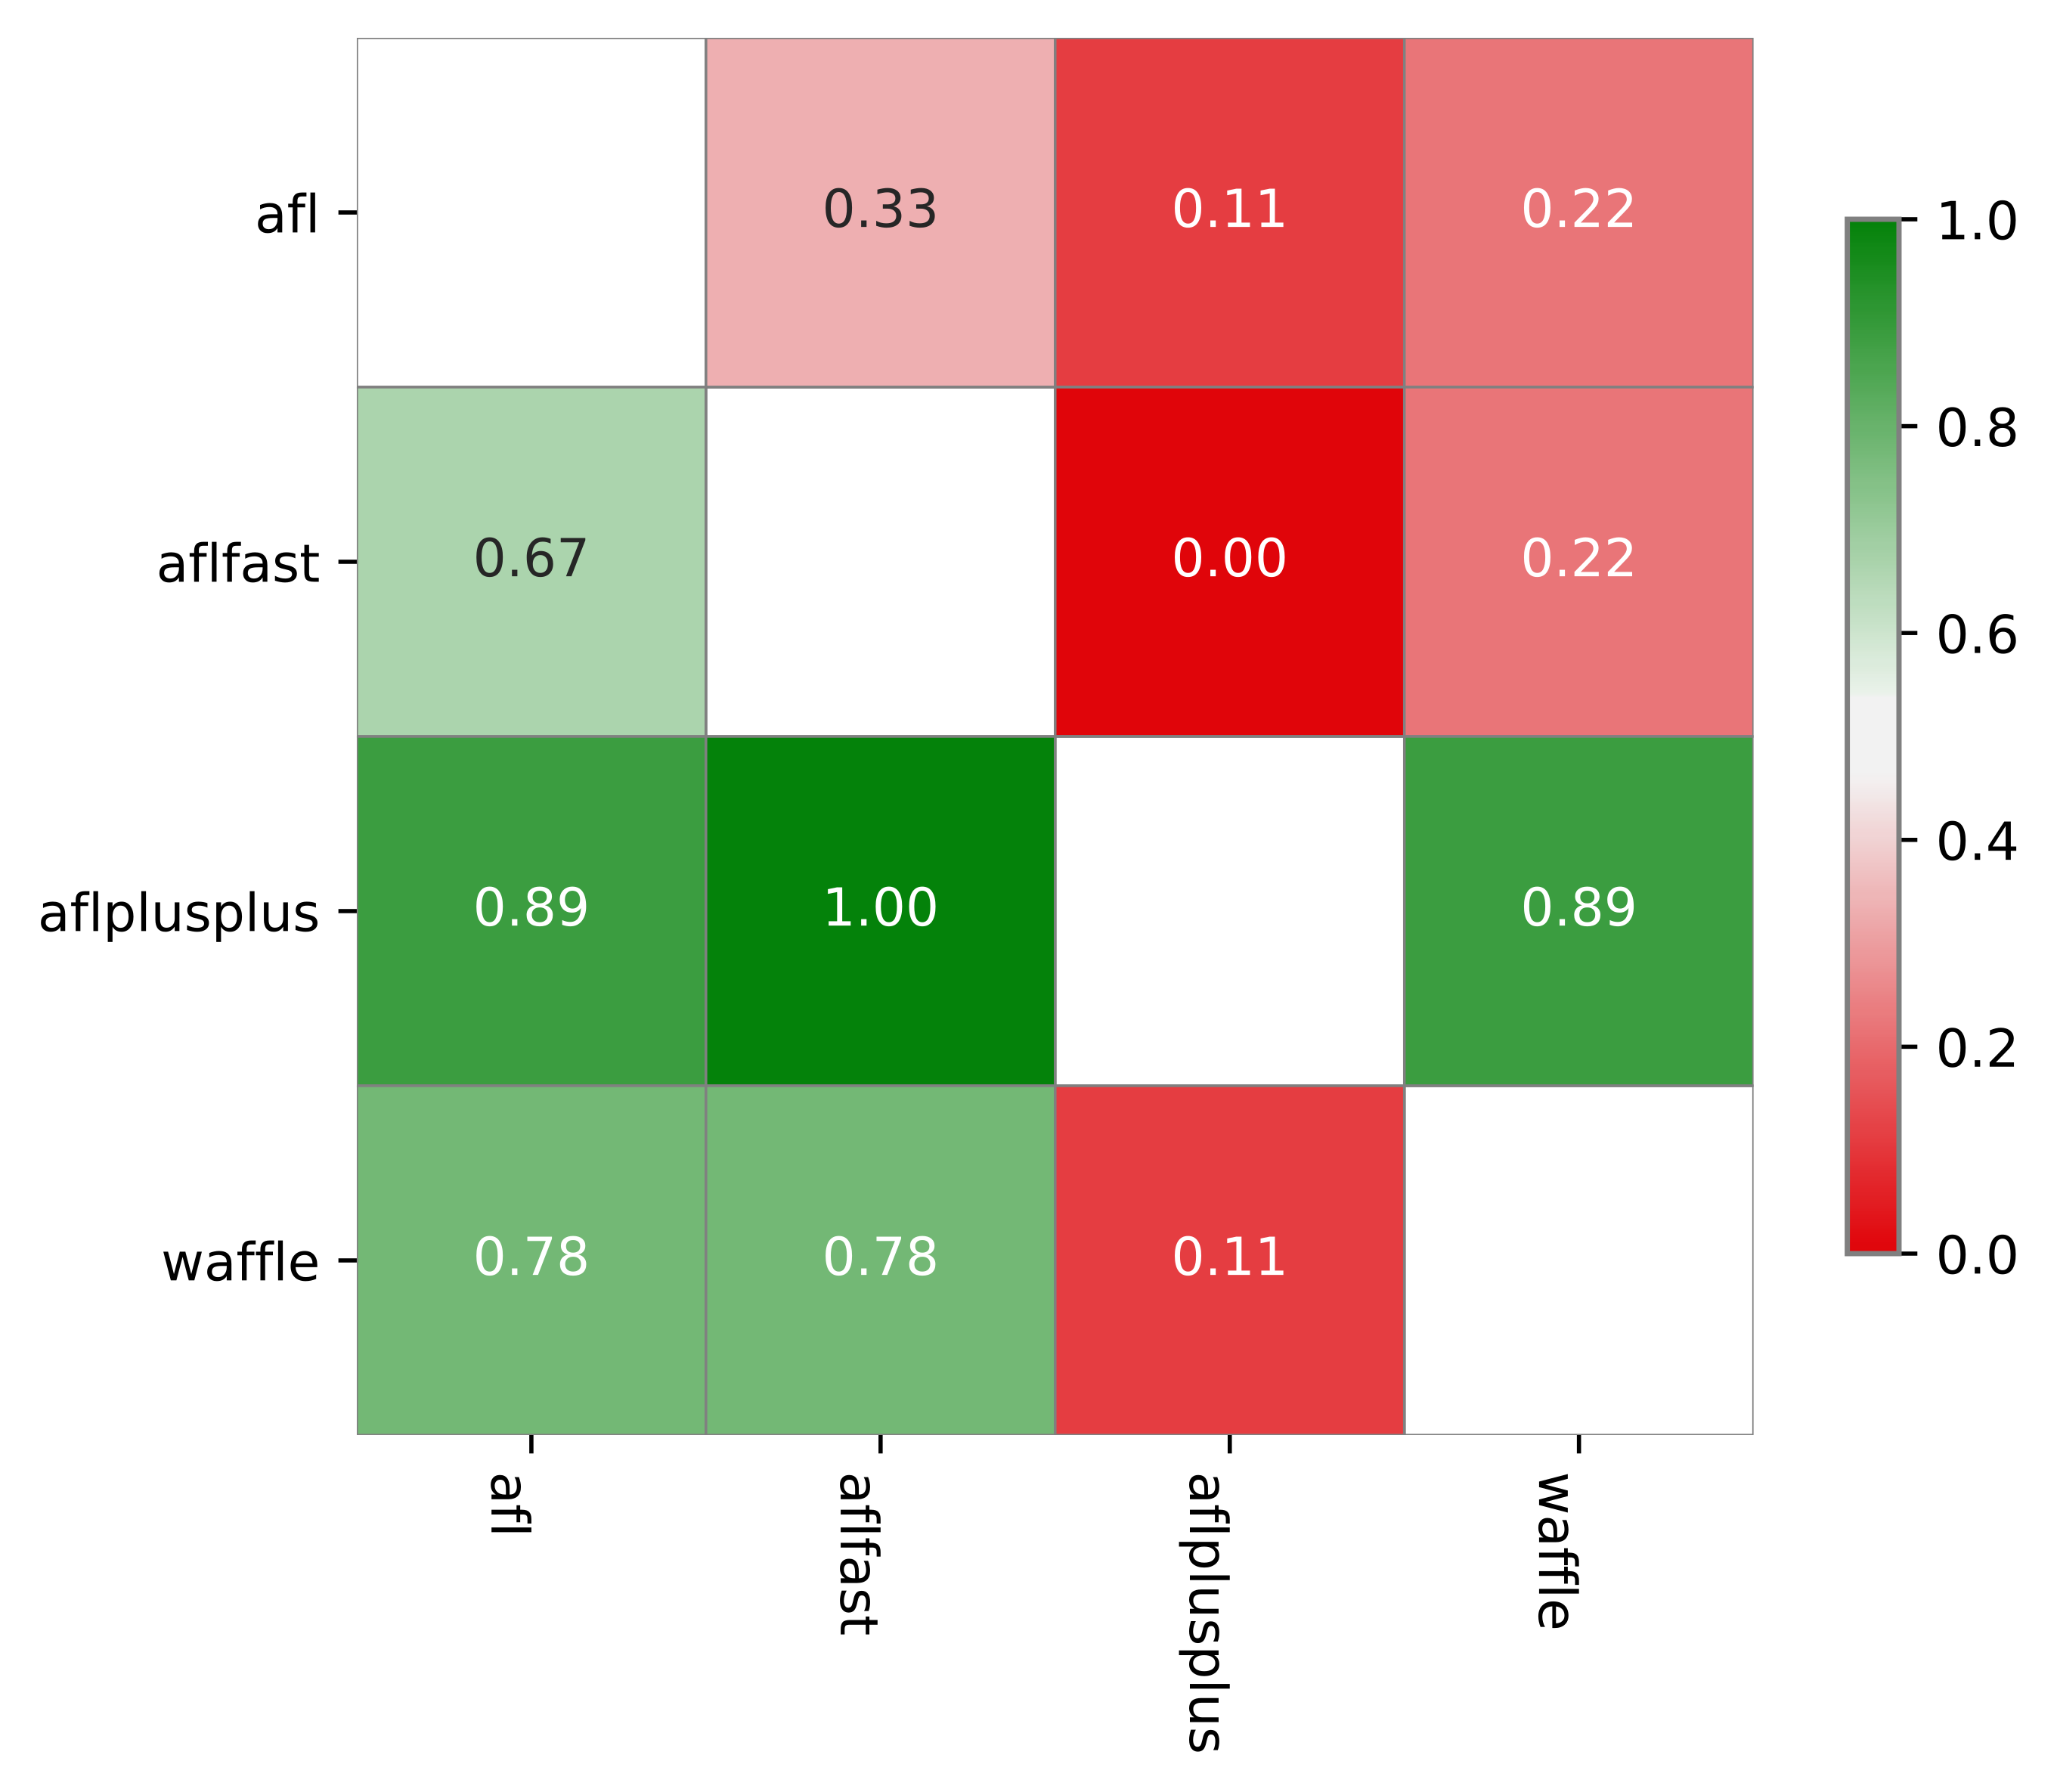
\includegraphics[width=0.95\linewidth]{Experiments/libjpeg-turbo-07-2017_varga_delaney_a12_plot.png}
%         \caption{libjpeg-turbo-07-2017}
%         \label{fig:sub:libjpeg-vda12}
%     \end{subfigure}

%     \begin{subfigure}[b]{0.475\linewidth}
%         \centering
%         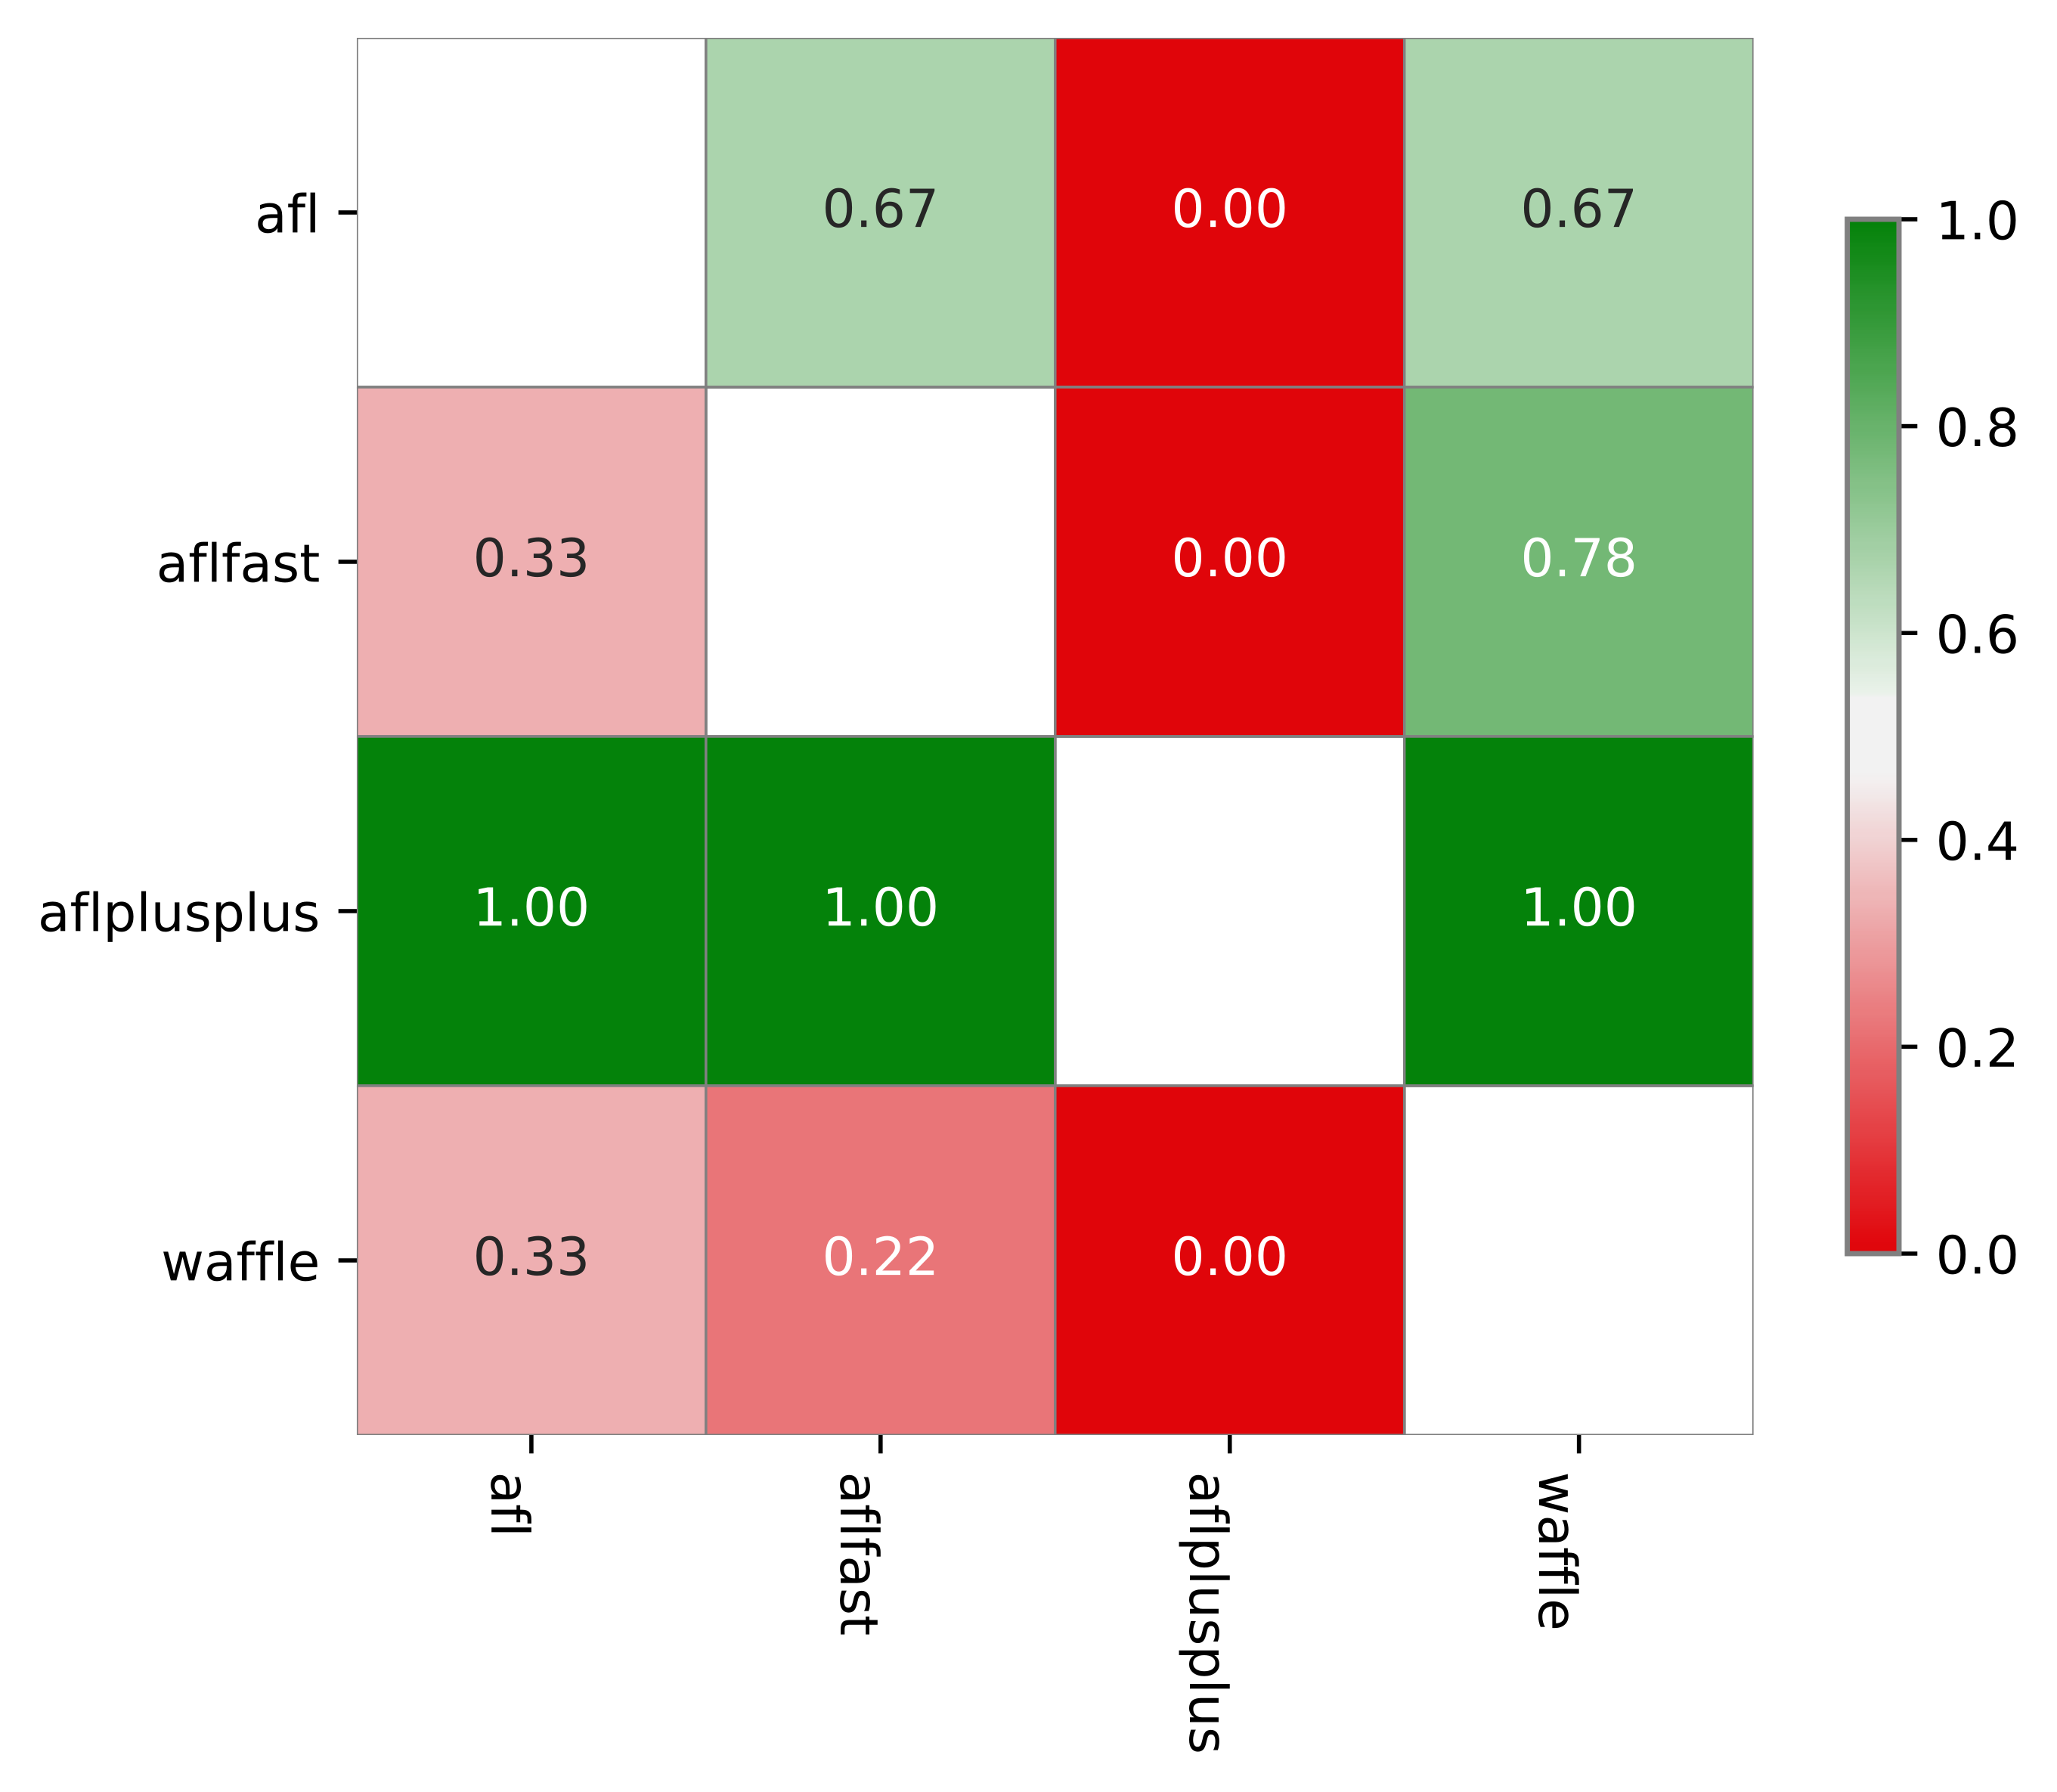
\includegraphics[width=0.95\linewidth]{Experiments/libpng-1.2.56_varga_delaney_a12_plot.png}
%         \caption{libpng-1.2.56}
%         \label{fig:sub:libpng-vda12}
%     \end{subfigure}
%     \begin{subfigure}[b]{0.475\linewidth}
%         \centering
%         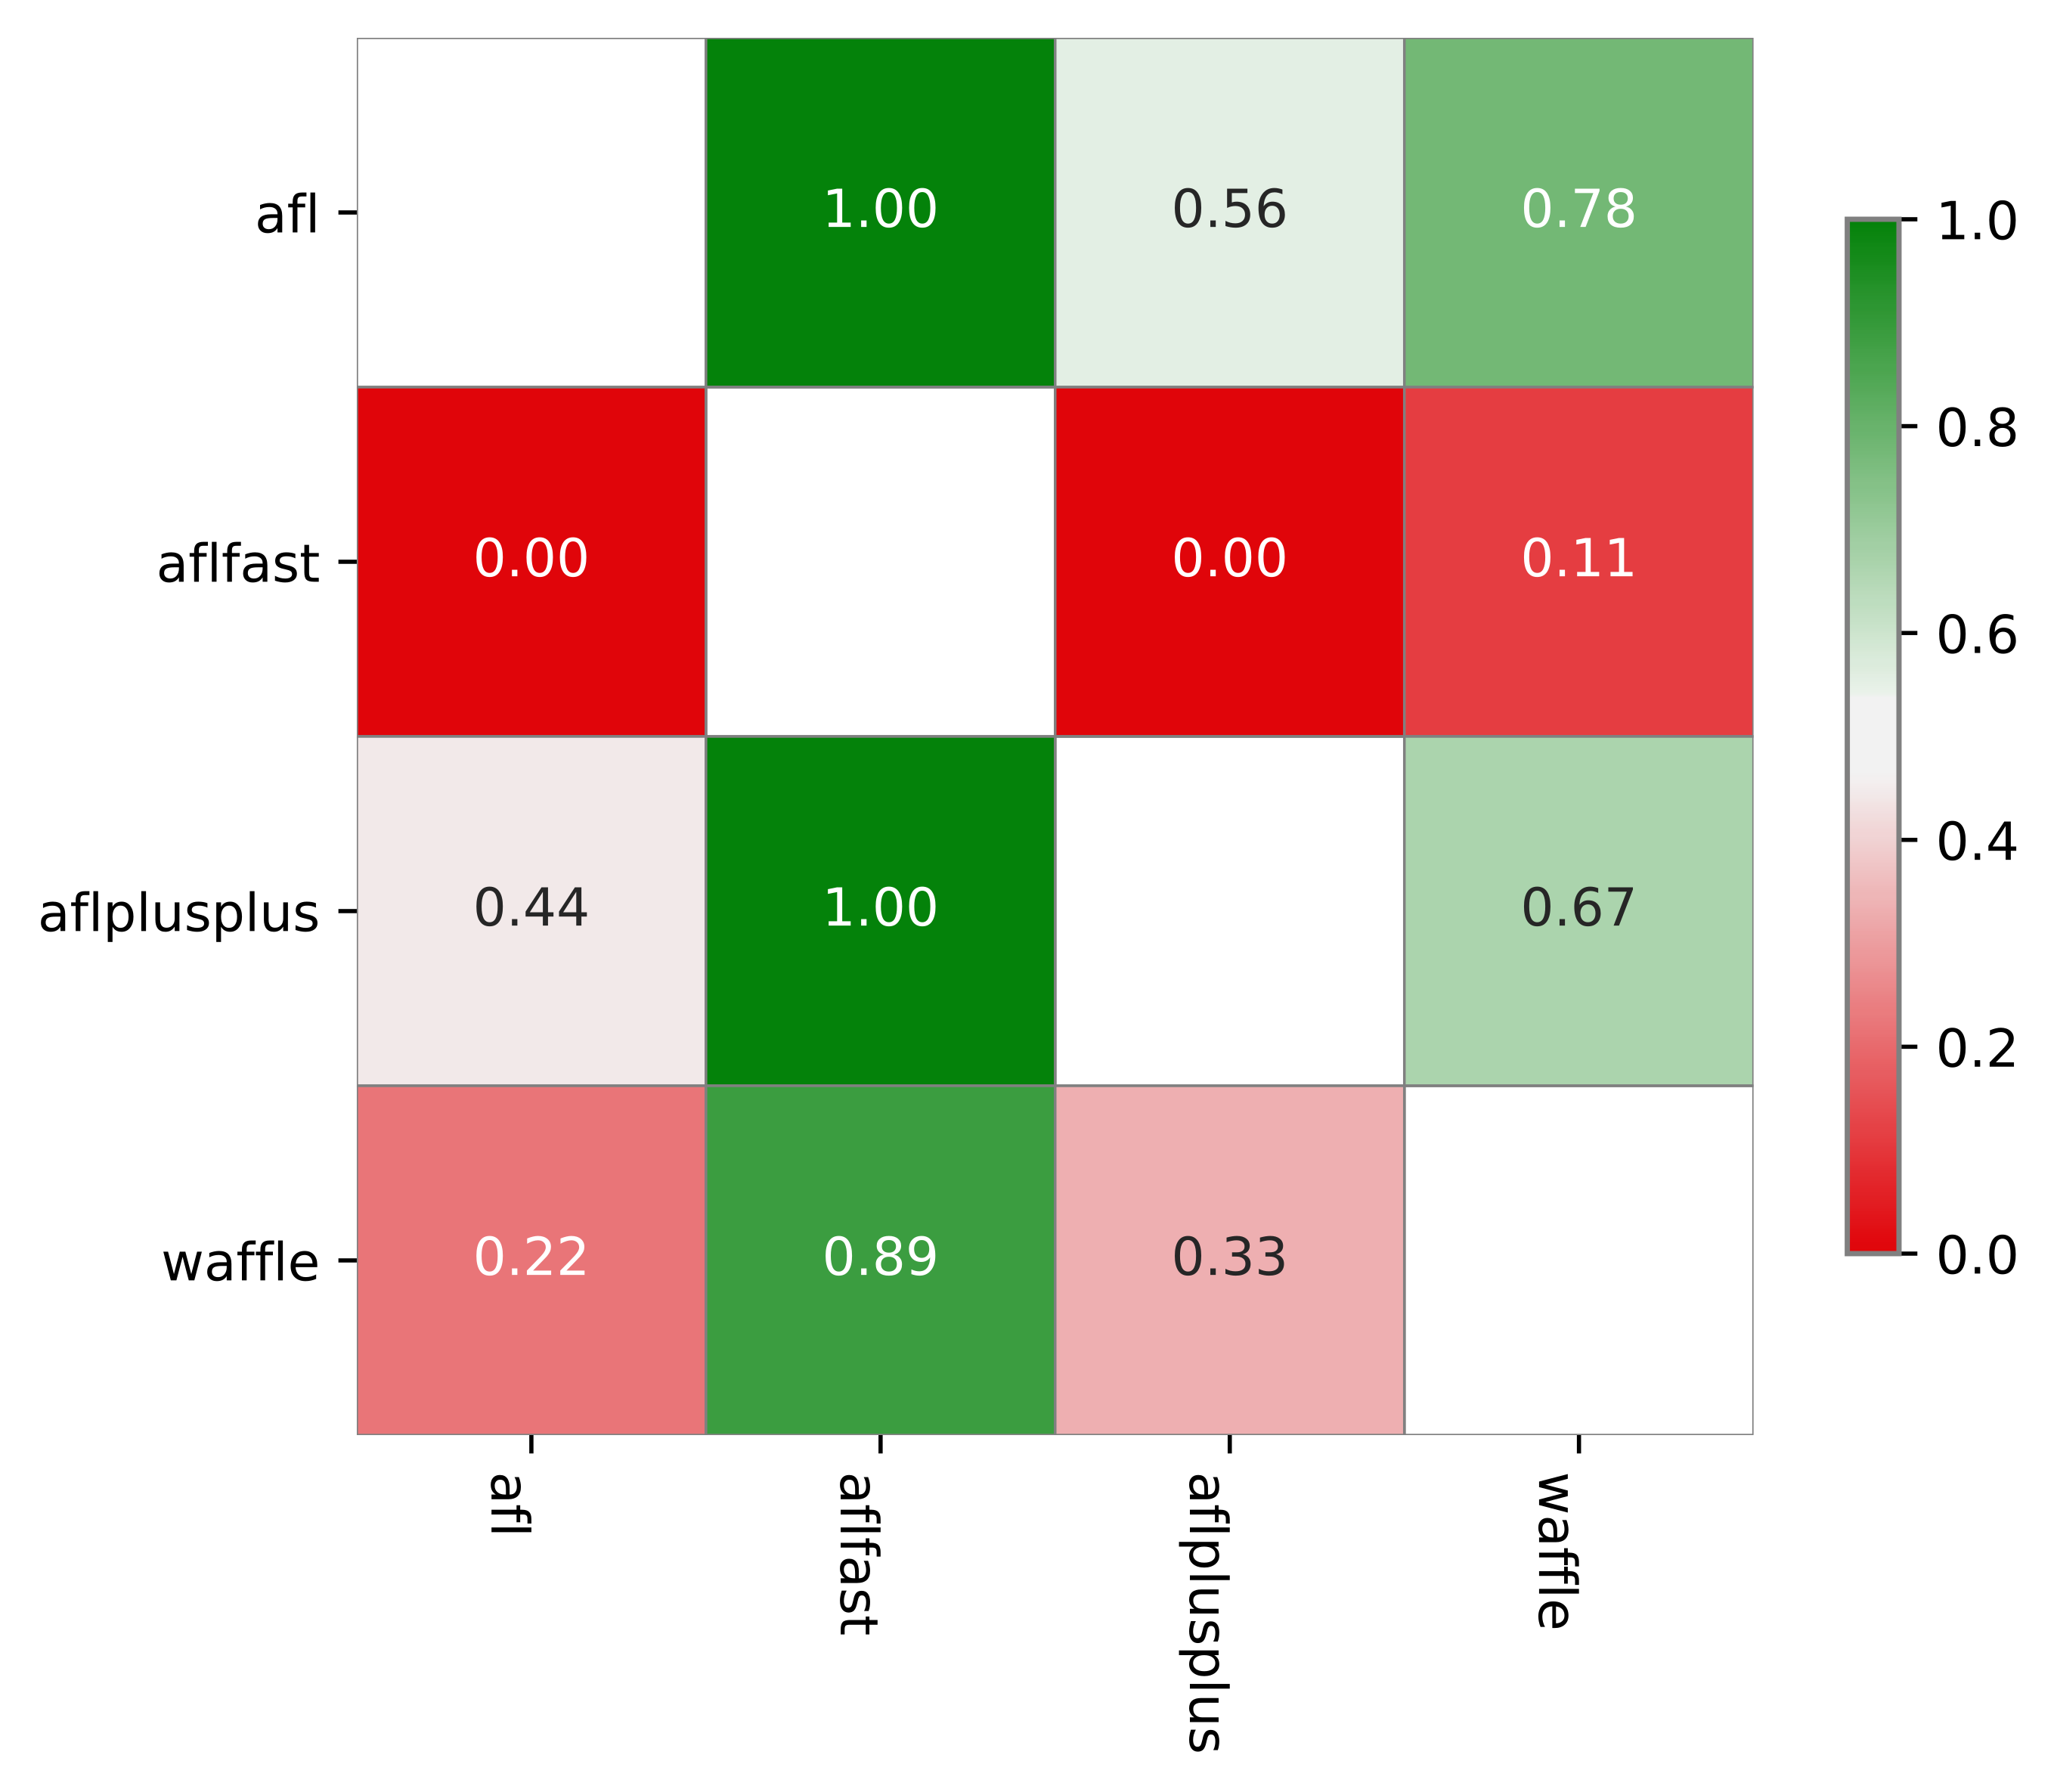
\includegraphics[width=0.95\linewidth]{Experiments/libxml2-v2.9.2_varga_delaney_a12_plot.png}
%         \caption{libxml2-v2.9.2}
%         \label{fig:sub:libxml-vda12}
%     \end{subfigure}

%     \caption{Unique coverage findings - The table summarizes the A12 values from the pairwise Vargha-Delaney A measure of effect size. Green cells indicate the probability the fuzzer in the row will outperform the fuzzer in the column.}
%     \label{fig:vda12}
% \end{figure}

% \begin{table}[!t]
%     \begin{tabular}{|l|c|c|c|c|} 
%         \hline
%         \textbf{Fuzzer}         & \textbf{Benchmarks} & \begin{tabular}[c]{@{}c@{}}\textbf{Coverage}\\ \textbf{STD}\end{tabular} & \begin{tabular}[c]{@{}c@{}}\textbf{Mean}\\ \textbf{Coverage}\end{tabular} & \begin{tabular}[c]{@{}c@{}}\textbf{Max}\\ \textbf{Coverage}\end{tabular} \\
%         \hline
%         \rowcolor{gray!20}      & freetype2 & 673.115 & 18968.3 & 19745.0 \\ \cline{2-5}
%                                 & libjpeg   & 155.094 &  3454.6 &  3628.0 \\ \cline{2-5}
%                                 \rowcolor{gray!20} & libpng    &  	0.577 &  1941.6 &  1942.0 \\ \cline{2-5}
%                                 & libxml    & 225.646 & 11246.3 & 11504.0 \\ \cline{2-5}
%         \hline
%         \rowcolor{gray!20} \multirow{4}{*}{AFL}    & freetype2 & 146.550 & 18520.0 & 18612.0 \\ \cline{2-5}
%                                 & libjpeg   &  51.156 &  3352.0 &  3411.0 \\ \cline{2-5}
%                                 & libpng    &   2.645 &  1943.0 &  1945.0 \\ \cline{2-5}
%                                 & libxml    & 355.017 & 11456.3 & 11851.0 \\ \cline{2-5}
%         \hline
%         \rowcolor{gray!20} \multirow{4}{*}{AFLFast}& freetype2 &  59.732 & 17508.0 & 17576.0 \\ \cline{2-5}
%                                 & libjpeg   &  41.761 &  3354.0 &  3402.0 \\ \cline{2-5}
%                                 & libpng    &   0.577 &  1942.3 &  1943.0 \\ \cline{2-5}
%                                 & libxml    & 152.346 & 10953.6 & 11093.0 \\ \cline{2-5}
%         \hline
%         \rowcolor{gray!20} \multirow{4}{*}{AFL++}  & freetype2 & 694.859 & 20961.3 & 21625.0 \\ \cline{2-5}
%                                 & libjpeg   & 195.438 &  3634.6 &  3749.0 \\ \cline{2-5}
%                                 & libpng    &  16.258 &  2092.6 &  2111.0 \\ \cline{2-5}
%                                 & libxml    & 84.571  & 11334.3 & 11431.0 \\ \cline{2-5}
%         \hline
%     \end{tabular}
%     \caption{Coverage stats}
%     \label{table:all-cov}
% \end{table}

Table \ref{table:all-cov} contains the coverage stats of the experiments. These stats describe an average coverage performance (on three trials) for each fuzzer on benchmarks. 

\begin{table}[!t]
    \centering
    \begin{tabular}{|c|c|c|c|c|} 
        \hline
        \textbf{Fuzzer}         & \textbf{Benchmarks} & \begin{tabular}[c]{@{}c@{}}\textbf{Coverage}\\ \textbf{STD}\end{tabular} & \begin{tabular}[c]{@{}c@{}}\textbf{Mean}\\ \textbf{Coverage}\end{tabular} & \begin{tabular}[c]{@{}c@{}}\textbf{Max}\\ \textbf{Coverage}\end{tabular} \\
        \hline
        \rowcolor{lightgray}\multirow[t]{4}{*}{\cellcolor{white}freetype}     
         & Waffle & 673.115 & 18968.3 & 19745.0 \\ \cline{2-5}
        & AFL & 146.550 & 18520.0 & 18612.0 \\ \cline{2-5}
        \rowcolor{lightgray} \cellcolor{white} & AFLFast &  59.732 & 17508.0 & 17576.0 \\ \cline{2-5}
        & AFL++ & 694.859 & 20961.3 & 21625.0 \\ \cline{2-5}
        
        \hline
        \rowcolor{lightgray} \multirow[t]{4}{*}{\cellcolor{white}libjpeg}    
        & Waffle   & 155.094 &  3454.6 &  3628.0 \\ \cline{2-5}
        & AFL   &  51.156 &  3352.0 &  3411.0 \\ \cline{2-5}
        \rowcolor{lightgray} \cellcolor{white} & AFLFast   &  41.761 &  3354.0 &  3402.0 \\ \cline{2-5}
        & AFL++   & 195.438 &  3634.6 &  3749.0 \\ \cline{2-5}
        
        \hline
        \rowcolor{lightgray} \multirow[t]{4}{*}{\cellcolor{white}libpng}
        & Waffle    &  	0.577 &  1941.6 &  1942.0 \\ \cline{2-5}
        & AFL    &   2.645 &  1943.0 &  1945.0 \\ \cline{2-5}
        \rowcolor{lightgray} \cellcolor{white} & AFLFast    &   0.577 &  1942.3 &  1943.0 \\ \cline{2-5}
        & AFL++    &  16.258 &  2092.6 &  2111.0 \\ \cline{2-5}
        
        \hline
        \rowcolor{lightgray} \multirow[t]{4}{*}{\cellcolor{white}libxml}  
        & Waffle    & 225.646 & 11246.3 & 11504.0 \\ \cline{2-5}
        & AFL    & 355.017 & 11456.3 & 11851.0 \\ \cline{2-5}
        \rowcolor{lightgray} \cellcolor{white} & AFLFast    & 152.346 & 10953.6 & 11093.0 \\ \cline{2-5}
        & AFL++    & 84.571  & 11334.3 & 11431.0 \\ \cline{2-5}
        \hline
    \end{tabular}
    \caption{Coverage stats}
    \label{table:all-cov}
\end{table}

\subsection{Execution time}

The performance of the fuzzers, based on execution times, is shown in histograms of instances of the tests (\cref{Figure:exe-freetype,Figure:exe-libjpeg,Figure:exe-libpng,Figure:exe-libxml}). In \cref{Figure:exe-freetype,Figure:exe-libpng,Figure:exe-libxml}, although the total number of findings in Waffle is less than AFL's, the Waffle's findings are spread more toward higher execution times.

\begin{figure}
    \centering
    \begin{subfigure}[t]{0.475\textwidth}
        \centering
        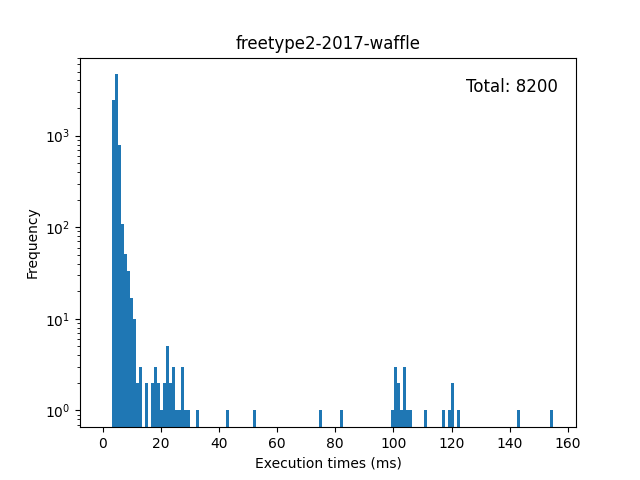
\includegraphics[width=\textwidth]{Experiments/execs/freetype2-2017-waffle.png}
        \caption{}
        \label{fig:sub:freetype-hist-waffle}
    \end{subfigure}
    \hfill
    \begin{subfigure}[t]{0.475\textwidth}
        \centering
        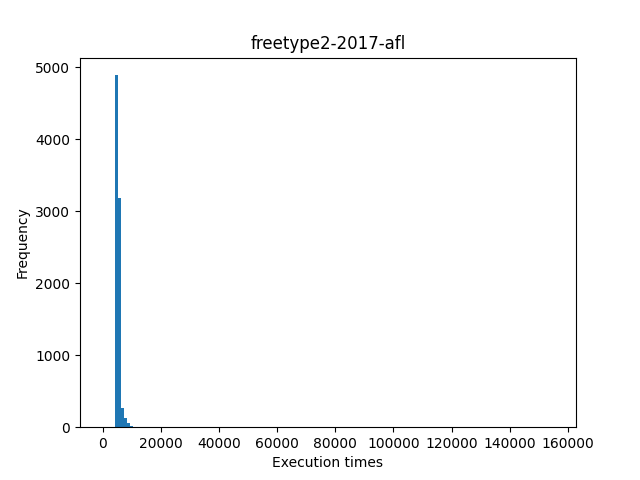
\includegraphics[width=\textwidth]{Experiments/execs/freetype2-2017-afl.png}
        \caption{}
        \label{fig:sub:freetype-hist-afl}
    \end{subfigure}
    \vskip\baselineskip
    \begin{subfigure}[t]{0.475\textwidth}
        \centering
        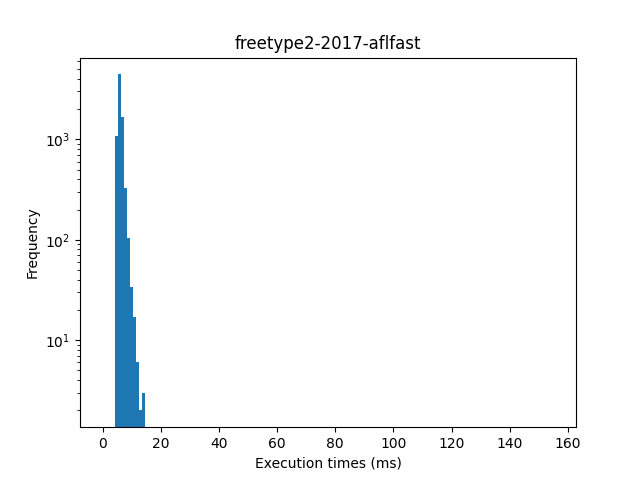
\includegraphics[width=\textwidth]{Experiments/execs/freetype2-2017-aflfast.png}
        \caption{}
        \label{fig:sub:freetype-hist-aflfast}
    \end{subfigure}
    \hfill
    \begin{subfigure}[t]{0.475\textwidth}
        \centering
        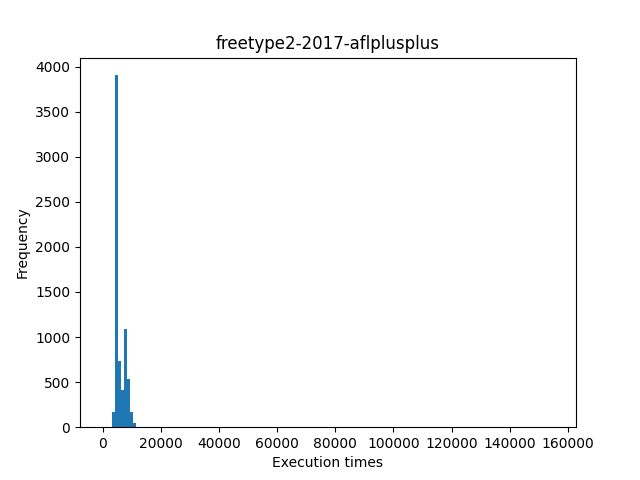
\includegraphics[width=\textwidth]{Experiments/execs/freetype2-2017-aflplusplus.png}
        \caption{}
        \label{fig:sub:freetype-hist-aflplusplus}
    \end{subfigure}

    \caption{Histogram of execution times: freetype2-2017}
    \label{Figure:exe-freetype}
\end{figure}


\begin{figure}
    \centering
    \begin{subfigure}[t]{0.475\textwidth}
        \centering
        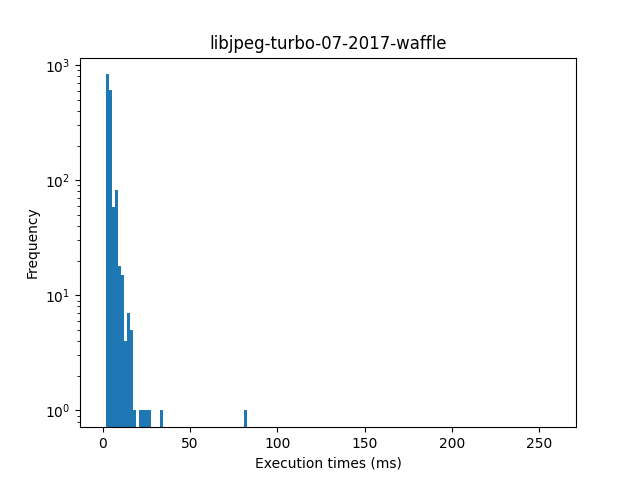
\includegraphics[width=\textwidth]{Experiments/execs/libjpeg-turbo-07-2017-waffle.png}
        \caption{}
        \label{fig:sub:libjpeg-hist-waffle}
    \end{subfigure}
    \hfill
    \begin{subfigure}[t]{0.475\textwidth}
        \centering
        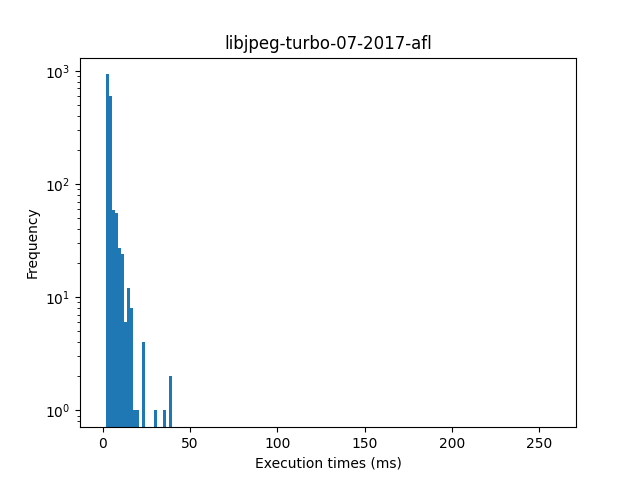
\includegraphics[width=\textwidth]{Experiments/execs/libjpeg-turbo-07-2017-afl.png}
        \caption{}
        \label{fig:sub:libjpeg-hist-afl}
    \end{subfigure}
    \vskip\baselineskip
    \begin{subfigure}[t]{0.475\textwidth}
        \centering
        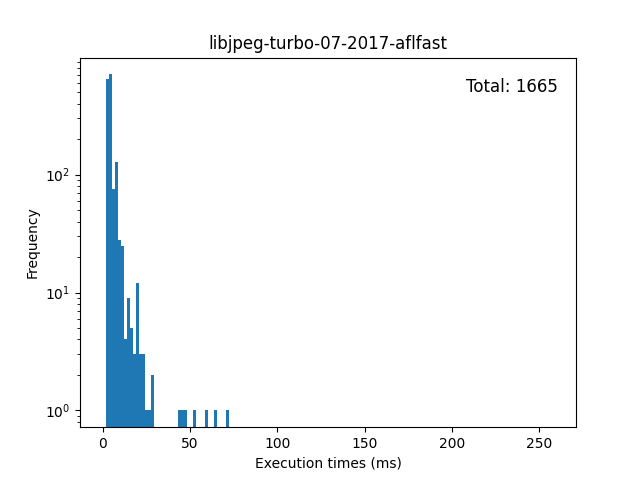
\includegraphics[width=\textwidth]{Experiments/execs/libjpeg-turbo-07-2017-aflfast.png}
        \caption{}
        \label{fig:sub:libjpeg-hist-aflfast}
    \end{subfigure}
    \hfill
    \begin{subfigure}[t]{0.475\textwidth}
        \centering
        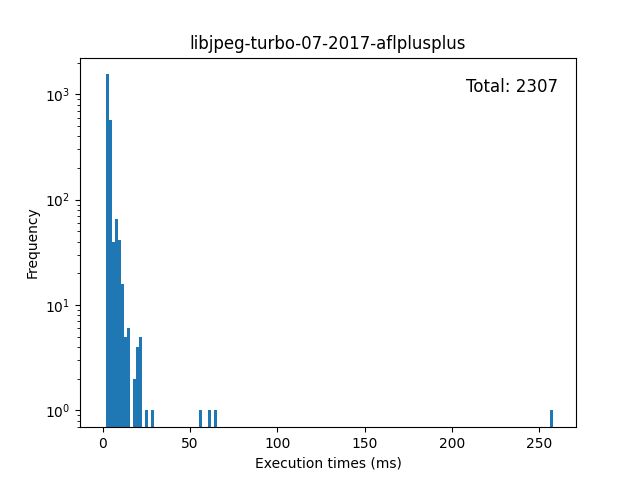
\includegraphics[width=\textwidth]{Experiments/execs/libjpeg-turbo-07-2017-aflplusplus.png}
        \caption{}
        \label{fig:sub:libjpeg-hist-aflplusplus}
    \end{subfigure}

    \caption{Histogram of execution times: libjpeg-turbo-07-2017}
    \label{Figure:exe-libjpeg}
\end{figure}

\begin{figure}
    \centering
    \begin{subfigure}[t]{0.475\textwidth}
        \centering
        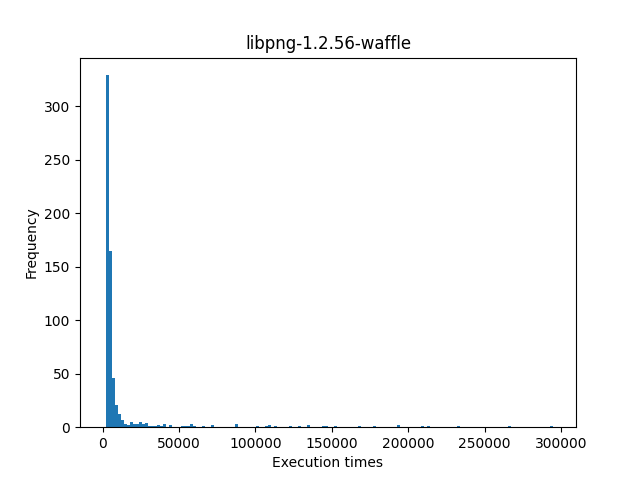
\includegraphics[width=\textwidth]{Experiments/execs/libpng-1.2.56-waffle.png}
        \caption{}
        \label{fig:sub:libpng-hist-waffle}
    \end{subfigure}
    \hfill
    \begin{subfigure}[t]{0.475\textwidth}
        \centering
        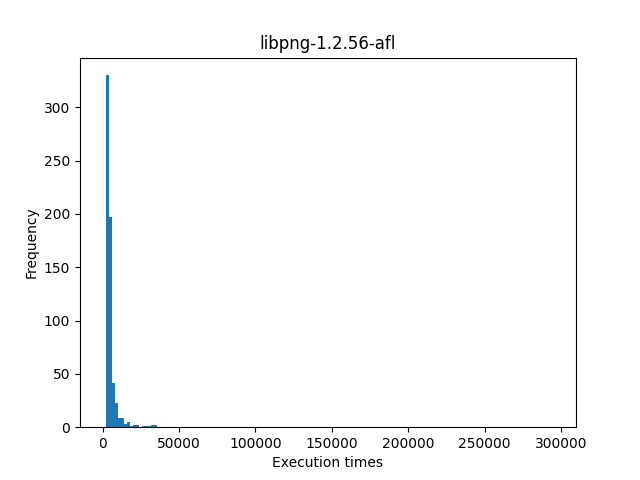
\includegraphics[width=\textwidth]{Experiments/execs/libpng-1.2.56-afl.png}
        \caption{}
        \label{fig:sub:libpng-hist-afl}
    \end{subfigure}
    \vskip\baselineskip
    \begin{subfigure}[t]{0.475\textwidth}
        \centering
        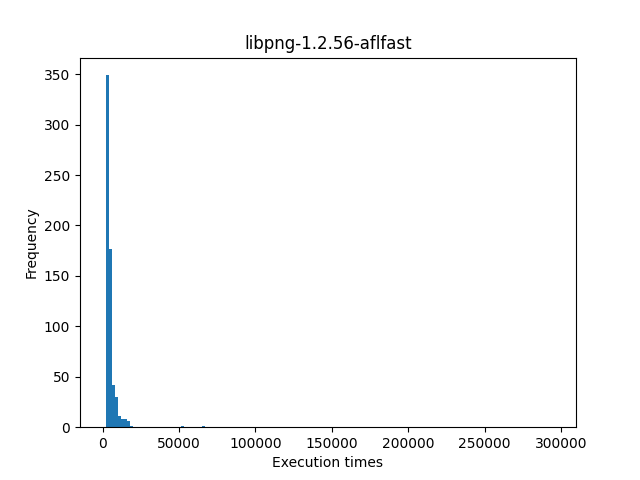
\includegraphics[width=\textwidth]{Experiments/execs/libpng-1.2.56-aflfast.png}
        \caption{}
        \label{fig:sub:libpng-hist-aflfast}
    \end{subfigure}
    \hfill
    \begin{subfigure}[t]{0.475\textwidth}
        \centering
        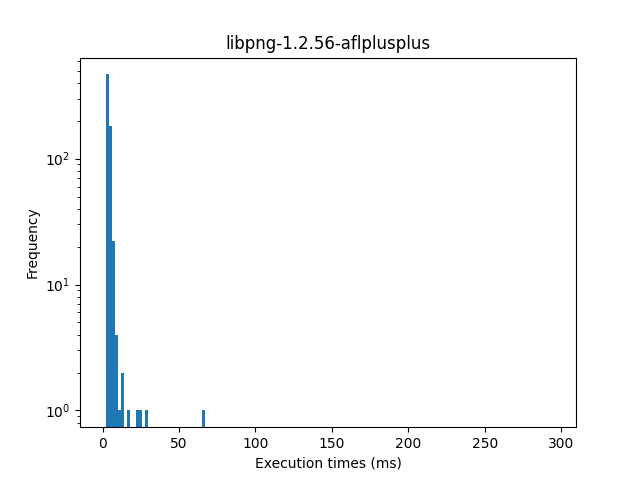
\includegraphics[width=\textwidth]{Experiments/execs/libpng-1.2.56-aflplusplus.png}
        \caption{}
        \label{fig:sub:libpng-hist-aflplusplus}
    \end{subfigure}

    \caption{Histogram of execution times: libpng-1.2.56}
    \label{Figure:exe-libpng}
\end{figure}

\begin{figure}
    \centering
    \begin{subfigure}[t]{0.475\textwidth}
        \centering
        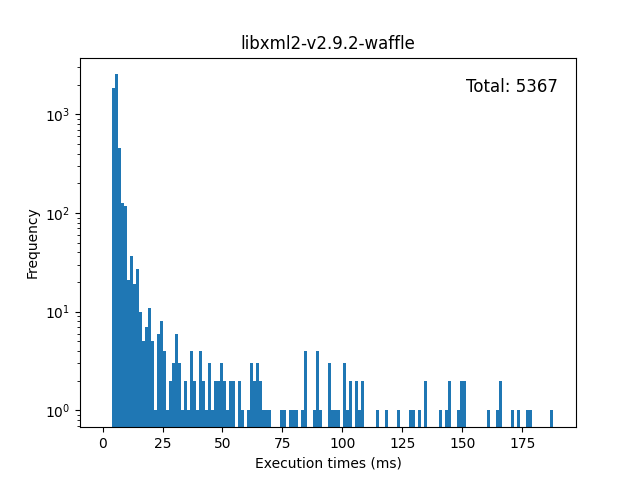
\includegraphics[width=\textwidth]{Experiments/execs/libxml2-v2.9.2-waffle.png}
        \caption{}
        \label{fig:sub:libxml2-hist-waffle}
    \end{subfigure}
    \hfill
    \begin{subfigure}[t]{0.475\textwidth}
        \centering
        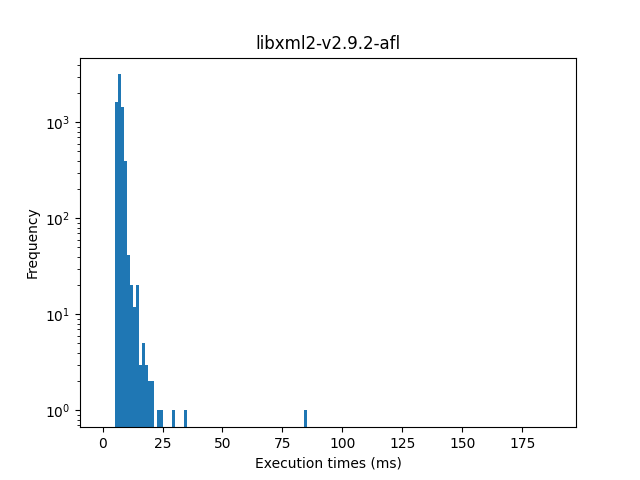
\includegraphics[width=\textwidth]{Experiments/execs/libxml2-v2.9.2-afl.png}
        \caption{}
        \label{fig:sub:libxml2-hist-afl}
    \end{subfigure}
    \vskip\baselineskip
    \begin{subfigure}[t]{0.475\textwidth}
        \centering
        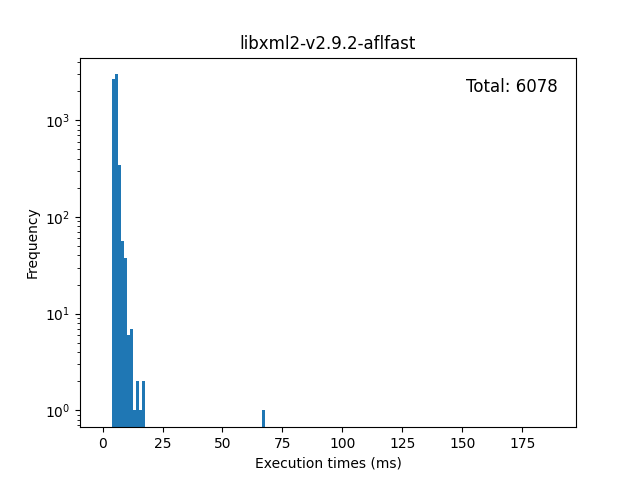
\includegraphics[width=\textwidth]{Experiments/execs/libxml2-v2.9.2-aflfast.png}
        \caption{}
        \label{fig:sub:libxml2-hist-aflfast}
    \end{subfigure}
    \hfill
    \begin{subfigure}[t]{0.475\textwidth}
        \centering
        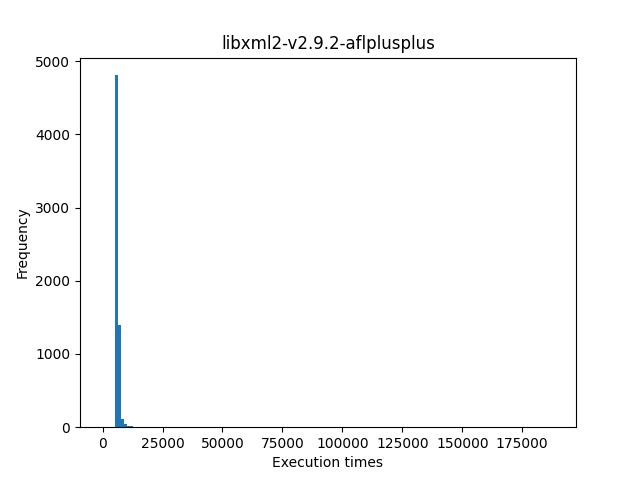
\includegraphics[width=\textwidth]{Experiments/execs/libxml2-v2.9.2-aflplusplus.png}
        \caption{}
        \label{fig:sub:libxml2-hist-aflplusplus}
    \end{subfigure}

    \caption{Histogram of execution times: libxml2-v2.9.2}
    \label{Figure:exe-libxml}
\end{figure}

Table \ref{table:all-exe} has the performance of \textbf{one} trial of each test, based on the execution time. 

\begin{table}[!t]
    \begin{adjustbox}{angle=90}
        {\setlength{\extrarowheight}{1ex}%
        \begin{tabular}{|c|c|c|c|c|c|c|c|} 
            \hline
            $Benchmarks$   & $Fuzzer$ & $Min_{(ms)}$ & $Max_{(ms)}$ & $Mean_{(ms)}$ & $Median_{(ms)}$ & $STD$ & $Total$ \\
            \hline
            \rowcolor{lightgray} \cellcolor{white} \multirow[t]{4}{*}{freetype} 
            & Waffle & 4.2 & 155.0 & 5.7 & 5.2 & 5.647 & 8201\\ \cline{2-8}
            & AFL & 4.3 & 12.7 & 5.2 & 5.0 & 0.668 & 8544 \\ \cline{2-8}
            \rowcolor{lightgray} \cellcolor{white} & AFLFast & 5.4 & 14.3 & 6.7 & 6.5 & 0.831 & 7647 \\ \cline{2-8}
            & AFL++ & 3.9 & 23.1 & 5.7 & 4.9 & 1.682 & 7056 \\ \cline{2-8}
            \hline
            \rowcolor{lightgray} \cellcolor{white} \multirow[t]{4}{*}{libjpeg}
            & Waffle   & 3.1 & 81.3 & 4.6 & 3.9 & 2.884 & 1637 \\ \cline{2-8}
            & AFL   & 3.3 & 38.2 & 4.7 & 3.9 & 2.674 & 1729 \\ \cline{2-8}
            \rowcolor{lightgray} \cellcolor{white} & AFLFast   & 3.3 & 71.6 & 5.3 & 4.1 & 4.374 & 1665 \\ \cline{2-8}
            & AFL++   & 3.0 & 258.8 & 4.4 & 3.7 & 6.025 & 2307 \\ \cline{2-8}
            \hline
            \rowcolor{lightgray} \cellcolor{white} \multirow[t]{4}{*}{libpng}
            & Waffle    & 2.8 & 295.1 & 12.1 & 3.9 & 31.245 & 643 \\ \cline{2-8}
            & AFL    & 2.7 & 34.8 & 5.0 & 3.8 & 3.882 & 629 \\ \cline{2-8}
            \rowcolor{lightgray} \cellcolor{white} & AFLFast    & 2.9 & 64.9 & 4.9 & 3.8 & 3.967 & 635 \\ \cline{2-8}
            & AFL++    & 2.8 & 65.1 & 4.1 & 3.5 & 3.003 & 684 \\ \cline{2-8}
            \hline
            \rowcolor{lightgray} \cellcolor{white} \multirow[t]{4}{*}{libxml} 
            & Waffle    & 5.2 & 188.0 & 8.3 & 6.2 & 13.071 & 5369 \\ \cline{2-8}
            & AFL    & 6.0 & 85.0 & 7.7 & 7.5 & 1.551 & 6757 \\ \cline{2-8}
            \rowcolor{lightgray} \cellcolor{white} & AFLFast    & 5.2 & 67.5 & 6.2 & 6.0 & 1.064 & 6078 \\ \cline{2-8}
            & AFL++    & 5.0 & 100.8 & 6.1 & 5.9 & 1.781 & 6426 \\ \cline{2-8}
            \hline
        \end{tabular}
        }
    \end{adjustbox}
    \caption{Execution times stats}
    \label{table:all-exe}
\end{table}

\section{Performance Bottlenecks of Waffle}
\label{sec:neck}

As we explained in Chapter \ref{chap:3}, after each execution of the target program, Waffle runs the function \texttt{has\_new\_icnt()} after \texttt{has\_new\_bits()}, for detecting the changes of the instruction counters on each edge. \texttt{has\_new\_icnt()} helps Waffle prioritize the edges that their instruction counters increase faster.

To investigate the performance changes for the insertion of \texttt{has\_new\_icnt()}, we ran this function on a sparse array of 32bit integers. On the other hand, we ran the function \texttt{has\_new\_bits()} on a sparse array of 8bit integers, for the same number of iterations. The results showed that the trial of \texttt{has\_new\_icnt()} takes \textbf{$~15000$} milliseconds, while the mentioned execution of \texttt{has\_new\_bits()} takes ~1500 milliseconds, on the local computer. As a result, the execution of both of the functions consecutively, takes \textbf{11x} longer.

% \section{Instrumentation}

To inject code into the binary of the target program, we modify the two files \textit{waffle-llvm-rt.o.c} and \textit{waffle-llvm-pass.so.cc}. The first file is responsible for the initial setup for the SHM and fork server. The later file injects the basic-block level instrumentation, which contains our feature collection procedure.

In the file \textit{waffle-llvm-rt.o.c} first, we specify an array of 64KB, in addition to the shared memory implemented in Memlock. This array collects the instruction counters and monitors the execution of the program through each basic-block.

\begin{lstlisting}[language=C++,style=CodeStyle,caption={waffle-llvm-rt.o.c},label={lst:memlock}]
    u32  __wafl_icnt_initial[ICNT_SIZE];
    u32* __wafl_icnt_ptr = __wafl_icnt_initial;
\end{lstlisting}

Here $ICNT\_SIZE$ is equal to $2^{14}$ words, which makes the size of 64KB. 

In the file \textit{waffle-llvm-pass.so.cc} we implement the LLVM pass, which helps us with injecting basic-block level instructions. For our purposes, we are using the instruction visitor, which we explained in Chapter \ref{chap:ch2}. 

After the above modifications on Memlock, we can \textit{make} the LLVM project within Waffle. Our improvements will be applied in the \textit{waffle-clang}, which we can use for compiling the target program.

To compile a source code to an executable, we specify the path to \textit{waffle-clang} as the compiler for building executable target programs. For instance, if the program contains a single source file, we can use the following command:

\begin{lstlisting}[language=bash,style=CommandStyle,caption=Compile a single file using waffle-clang]
    ./waffle-clang -i <sourcecode-path> -o <executable-path>
\end{lstlisting}

Choosing the right compiler here is necessary as \textit{waffle-clang/waffle-clang++} injects the proposed instrumentation. Generally, we can define the path to the compiler by exporting it to the environment variables:

\begin{lstlisting}[language=bash,style=CommandStyle,caption=Compile using waffle-clang]
    export CC=waffle-clang
    export CXX=waffle-clang++
\end{lstlisting}

Waffle uses the resulting executables for its fuzzing procedure.


% \section{Start fuzzing}

Waffle takes the current entry from the queue, fuzzes it for a while, and when finished, turns back to the queue for another entry.

To use the instrumentation features, Waffle participates in sharing memory with the target program. The instantiated shared memory will be passed to the target program every time the fuzzer executes the program.

After the execution of the target program, collected data are stored in three arrays, $trace\_bits$, $perf\_bits$, and $icnt\_bits$. These arrays contain the information for coverage, stack memory consumption, and the counters for each basic block's instructions. The total size of the shared memory is 128KB.

Memlock calculates a \textit{stallness} for measuring the performance of the fuzzer. If the behavior of execution of input is too stall, Memlock skips fuzzing the current input entry and continues with the next entry of the queue. In Waffle, we do not intend to measure stallness, and we switch between fuzzing approaches, as mentioned before.

AFL trims the test-cases to increase the performance of coverage-finding techniques. As trimming the results may affect the target program's resource consumption, Memlock and Waffle disable this method in the fuzzing stage. 

Next, Waffle assesses its interest in considering the input as a favorable input. 

\begin{lstlisting}[language=C++,style=CodeStyle,caption={Update bitmap scores},label={lst:update_bitmap}]
  total_counts = 0;
  for (i = 0; i < ICNT_SIZE; i++) {
    if (icnt_bits[i]) {
      total_counts += icnt_bits[i];       
      if (top_rated[i]) {
        if (icnt_bits[i] < max_counts[i]) continue;
      }
      /* Insert ourselves as the new winner. */
      top_rated[i] = q;

      /* if we get here, we know that icnt_bits[i]==max_counts[i] */
      score_changed = 1;
    }
  }
  if(total_counts >= max_total_counts){
    top_rated[i] = q;
    score_changed = 1;
  } 
\end{lstlisting}

Here $ICNT\_SIZE$ is equal to the size of the bitmap for collecting the instruction counters. In case we find a new max for the number of instructions in a basic-block, we select the current input as the winner - favorable. [listing \ref{lst:update_bitmap}]

We are also selecting inputs with a total number of instructions more than any other input that was executed before.

\begin{lstlisting}[language=C++,style=CodeStyle,caption={Cull queue},label={lst:cull_queue}]
if (top_rated[i]) {
  /* if top rated for any i, will be favored */
  u8 was_favored_already = top_rated[i]->favored;

  top_rated[i]->favored = 1;

  /* increments counts only if not also favored for another i */
  if (!was_favored_already){
    queued_favored++;
    if (!top_rated[i]->was_fuzzed) pending_favored++;
  }
}

\end{lstlisting}

After collecting the execution features for an input, Waffle continues culling the queue and selects unique favorite inputs for the next generations. [listing \ref{lst:cull_queue}]

Notice that AFL and Memlock do the same method for selecting favorite inputs, except that they do not consider an overall execution feature, which Waffle knows as $max\_total\_counts$.

% \section{Monitoring fuzzing procedure}

To measure the performance of AFL, we can use the live status screen. 

\begin{figure}[H]
    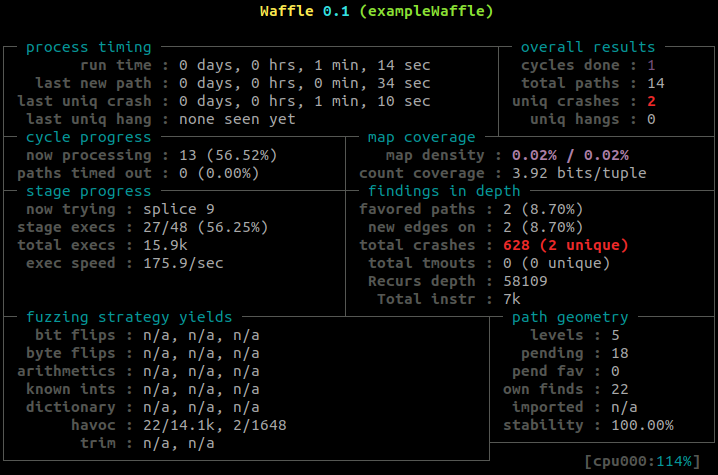
\includegraphics[width=\textwidth]{Chapter4/waffle-screen.png}
    \centering
    \label{img:waffle-screen}
    \caption{Status screen}
\end{figure}

In the above screen, the total number of instructions executed and the maximum depths for the stack is presented. Eventually, as the  

% \section{Summary}

In this chapter, we covered the following topics:

\begin{itemize}
    \item The implementation of the instrumentation
    \item The modifications in the fuzzing procedure
    \item We also improved the status screen to illustrate the details of the fuzzing procedure and for future assessments
\end{itemize}
% \section{Generating fuzzed data}
% \section{Report vulnerabilities}

% This is a subsection. This is \hfill a subsection.


\bibliographystyle{unsrt}
\bibliography{mybibliography}

\chapter{Appendix}

\begin{subappendices}
    % ! Waffle
    \section{Waffle}
    \label{app:waffle}
    
    % random_havoc stage
    \subsection{random\_havoc}
    \label{app:havoc}
    An abstract implementation of the \texttt{havoc\_stage} used in AFL and Waffle. Most of the commands are removed, and the remaining comments describe the operations of this stage.
    \lstinputlisting[language=C,style=CodeStyle,label={code:havoc},caption={Random havoc stage}]{Codes/Chapter2/havoc.c}    

\newpage
    % ! Fuzzbench
    \section{FuzzBench}
    \label{app:fuzzbench}

    We have reviewed the recipe for adding Waffle to FuzzBench in this section.

    \subsection{builder.Dockerfile}
    \label{app:builder.docker}
    Builds Waffle for the usage in FuzzBench.

    The \texttt{parent\_image} is an image instance with premitive configurations, and is on \texttt{ubuntu:xenial} OS. Building Python, installing python requirements, and installing the \texttt{google-cloud-sdk}, are the operations applied on the \texttt{parent\_image}.

    \lstinputlisting[language=docker-compose,style=CodeStyle,label={code:builder},caption={Recipe for building Waffle FuzzBench}]{Codes/Chapter4/builder.Dockerfile}

    \subsection{fuzzer.py}
    \label{app:fuzzer.py}
    This python program specifies the sequence of the actions Waffle takes, in order to start fuzzing and use the benchmark as the target program. This program modifies the file located in \texttt{\{FUZZBENCH\_DIR\}/fuzzers/AFL/fuzzer.py}. As Waffle is based on AFL, this program can start the process same as the AFL's \texttt{fuzzer.py}.

    \lstinputlisting[language=Python,style=CodeStyle,label={code:fuzz.py},caption={Recipe for running fuzzing with Waffle on a target}]{Codes/Chapter4/fuzzer.py}


\end{subappendices}

% %%-------------Glossary--------------------------------
\chapter*{Glossary (if any)}
\addcontentsline{toc}{chapter}{Glossary} start writing here.

% %%-------------Vita---------------------------------
\clearpage
\phantomsection  % correct link in PDF bookmarks.
\addtocontents{toc}{\cftpagenumbersoff{chapter}}  % omit page # in ToC
\addcontentsline{toc}{chapter}{Vita}
\chapter*{Vita}
\pagestyle{empty}
\thispagestyle{empty}
\singlespacing
Candidate's full name:
\textbf{Behnam Bojnordi Arbab}\\
University attended:
\textbf{University of New Brunswick (UNB),\\
Master of Computer Science, 2022}\\
Github repository: https://github.com/behnamarbab

\end{document}
